\documentclass[a4paper]{article}
\usepackage{svg}
\usepackage{vntex}
\usepackage{pdflscape}
\usepackage{subcaption}
\usepackage{rotating}
\usepackage{a4wide,amssymb,epsfig,latexsym,multicol,array,hhline,fancyhdr}
\usepackage{booktabs}
\usepackage{float}
\usepackage{longtable}
\usepackage{placeins}
\usepackage{capt-of}
\usepackage{tabularx}
\usepackage{caption}
\usepackage{amsmath}
\usepackage{lastpage}
\usepackage{enumerate}
\usepackage{color}
\usepackage{graphicx}
\usepackage{multirow}
\usepackage[framemethod=tikz]{mdframed}
\usepackage{wrapfig}
\usepackage{geometry}
\usepackage{setspace}
\usepackage{tikz}
\usetikzlibrary{arrows,snakes,backgrounds,positioning,shapes}
\usepackage{hyperref}
\usepackage{indentfirst}
\usepackage{cases}
\usepackage{xcolor}
\usepackage[most]{tcolorbox}
\usepackage[shortlabels]{enumitem}

\renewcommand{\baselinestretch}{1.45}
\renewcommand{\figurename}{Hình}
\renewcommand{\tablename}{Bảng}

\newtcolorbox{softbox}{
    colback=black!3,
    colframe=black!3,
    arc=8pt,
    boxrule=0pt,
    left=10pt, right=10pt, top=8pt, bottom=8pt,
    fontupper=\itshape\color{black!80}
}

\hypersetup{
    colorlinks=true,
    linkcolor=black,
    citecolor=red,
    urlcolor=blue,
    filecolor=magenta
}

\setlength{\headheight}{40pt}
\pagestyle{fancy}
\fancyhead{}
\fancyhead[L]{
 \begin{tabular}{rl}
    \begin{picture}(25,15)(0,0)
    \put(0,-8){
\includegraphics[width=8mm, height=8mm]{images/khtn.png}}
    \end{picture}&
	\begin{tabular}{l}
		\textbf{\bf \ttfamily Ho Chi Minh University of Science - VNUHCM}\\
		\textbf{\bf \ttfamily Faculty of Information Technology}
	\end{tabular}  	
 \end{tabular}
}
\fancyhead[R]{
	\begin{tabular}{l}
		\tiny \bf \\
		\tiny \bf 
	\end{tabular}  }
\fancyfoot{}
\fancyfoot[L]{\scriptsize \ttfamily Introduction to Data Science -- arXiv Term Project}
\fancyfoot[R]{\scriptsize \ttfamily Trang {\thepage}/\pageref{LastPage}}
\renewcommand{\headrulewidth}{0.3pt}
\renewcommand{\footrulewidth}{0.3pt}

\setcounter{secnumdepth}{4}
\setcounter{tocdepth}{3}
\makeatletter
\newcounter {subsubsubsection}[subsubsection]
\renewcommand\thesubsubsubsection{\thesubsubsection .\@alph\c@subsubsubsection}
\newcommand\subsubsubsection{\@startsection{subsubsubsection}{4}{\z@}%
                                    {-3.25ex\@plus -1ex \@minus -.2ex}%
                                    {1.5ex \@plus .2ex}%
                                    {\normalfont\normalsize\bfseries}}
\newcommand*\l@subsubsubsection{\@dottedtocline{3}{10.0em}{4.1em}}
\newcommand*{\subsubsubsectionmark}[1]{}
\makeatother

\begin{document}

\begin{titlepage}
\thispagestyle{empty}
\begin{center}
VIETNAM NATIONAL UNIVERSITY HO CHI MINH CITY\\
HO CHI MINH CITY UNIVERSITY OF SCIENCE \\
FACULTY OF INFORMATION TECHNOLOGY
\end{center}

\vspace{0.5cm}

\begin{figure}[h!]
\begin{center}

\includegraphics[width=4.4cm]{images/khtn.png}
\end{center}
\end{figure}

\vspace{0.5cm}

\begin{center}
\begin{tabular}{c}
\multicolumn{1}{c}{\textbf{{\normalsize PROJECT REPORT}}}\\
~~\\
\hline
\\
\textbf{{\Large arXiv Crawling, Parsing, and Reference Matching}}\\
\\
\hline
\end{tabular}
\end{center}

\vspace{0.8cm}

\begin{table}[h!]
\centering
\begin{tabular}{rll}
\textbf{Môn học:} & Introduction to Data Science & \\
\textbf{Giảng viên:} &  & \\
\textbf{Thành viên:} & Nguyễn Phúc Khang & 24120068\\
 & Phạm Minh Trọng & 24120151\\
 & Trịnh Huỳnh Nhi & 24120404\\
 & Huỳnh Huy Hoàng & \textit{[Cập nhật MSSV]}\\
 & Ngô Mẫn Nhi & \textit{[Cập nhật MSSV]}\\
\end{tabular}
\end{table}

\vfill

\begin{center} {\footnotesize Thành phố Hồ Chí Minh, \today}
\end{center}
\end{titlepage}


\pagenumbering{roman}
\renewcommand{\contentsname}{Mục lục}
\renewcommand{\tablename}{Bảng}
\renewcommand{\figurename}{Hình}
\renewcommand{\refname}{Tài liệu tham khảo}
\renewcommand{\listfigurename}{Danh mục hình vẽ}
\renewcommand{\listtablename}{Danh mục bảng biểu}

\tableofcontents
\newpage
\listoffigures
\vspace{1.2cm}
\listoftables

\newpage
\pagenumbering{arabic}
\renewcommand{\arraystretch}{1.28}
\setcounter{page}{1}

\section{Tổng quan bài toán và kiến trúc hệ thống}

\subsection{Bối cảnh và phạm vi kho dữ liệu khoa học arXiv}

Các hệ thống khai phá văn bản khoa học hiện đại thường đối mặt với đánh đổi căn bản giữa khả năng tiếp cận thuận tiện của định dạng PDF và độ trung thực cấu trúc của mã nguồn gốc. Định dạng PDF được thiết kế chủ yếu phục vụ hiển thị trang in, do đó quá trình kết xuất đã làm thất lạc ranh giới phân cấp giữa các mục lớn nhỏ, phá vỡ cấu trúc ký hiệu toán học thành tọa độ phông chữ rời rạc, làm nhiễu thứ tự đọc ở bố cục nhiều cột và cắt đứt liên kết tường minh giữa câu văn với khóa trích dẫn thư mục. Trái lại, khoảng $97\%$ bài nộp trên kho lưu trữ học thuật arXiv cung cấp trực tiếp gói mã nguồn LaTeX nguyên bản~\cite{ginev2024}, cho phép bảo toàn đầy đủ cây cấu trúc tài liệu, công thức toán học chuẩn tắc, mục lục BibTeX và bối cảnh trích dẫn nội tuyến. Không dừng lại ở bản công bố cuối cùng, việc thu hoạch và phân tích đồng thời toàn bộ chuỗi lịch sử phiên bản của từng bài báo (từ phiên bản nộp đầu tiên $v_1$ đến tối đa $v_{13}$ trong tập dữ liệu khảo sát) mở ra khả năng theo dõi tiến hóa nội dung khoa học, đồng thời đặt ra bài toán khử trùng lặp cấu trúc ở quy mô hàng chục triệu nút. Khi kết hợp nguồn toàn văn giàu cấu trúc này với đồ thị trích dẫn liên kết từ nền tảng dữ liệu mở Semantic Scholar~\cite{kinney2023}, hệ thống hình thành nền tảng dữ liệu định lượng phục vụ trực tiếp bài toán học máy đối sánh tài liệu tham khảo theo chuẩn yêu cầu của đồ án môn Nhập môn Khoa học Dữ liệu~\cite{hcmus_intro_ds}.

Phạm vi dữ liệu của nhóm ChickenDev bao phủ năm dải mã định danh arXiv không giao nhau trong giai đoạn từ tháng $09/2024$ đến tháng $07/2025$, tạo thành kho dữ liệu chính thức gồm chính xác $25{,}000$ bài báo khoa học chia đều $5{,}000$ bài cho mỗi thành viên. Trong số này, ba dải nằm trọn trong một tháng dương lịch ($09/2024$, $01/2025$ và $03/2025$) nên chỉ cần kiểm tra đúng $5{,}000$ mã ứng viên mỗi dải, còn hai dải bắc ngang ranh giới chuyển tháng ($04\text{--}05/2025$ và $06\text{--}07/2025$) buộc hệ thống phải dò quét tuần tự lần lượt $83{,}142$ và $80{,}870$ mã ứng viên nhằm bảo đảm không bỏ sót bài báo hợp lệ nào gần ngưỡng kết thúc tháng vốn không được công bố trước. Tính tổng thể trên cả năm dải, quy trình dò tìm đã kiểm định $179{,}012$ mã ứng viên để xác nhận $25{,}000$ bài báo chính thức với $40{,}896$ phiên bản khai báo (trung bình $1.636$ phiên bản mỗi bài) và thu hoạch được $466{,}763$ liên kết tài liệu tham khảo có định danh arXiv. Ở tầng phân tích cấu trúc, $22{,}961$ bài báo ($91.84\%$) trải rộng trên $37{,}967$ phiên bản có mã nguồn TeX hợp lệ đã được bóc tách và nén khử trùng lặp xuống còn $11{,}098{,}189$ phần tử nội dung duy nhất nối nhau bởi $16{,}185{,}255$ cạnh quan hệ phân cấp, song hành với $975{,}674$ mục lục BibTeX hợp nhất. Từ toàn bộ kho dữ liệu chuẩn hóa này, một tập mẫu phân tầng gồm $2{,}525$ bài báo ($25$ bài gán nhãn thủ công và $2{,}500$ bài gán nhãn tự động) chứa $101{,}441$ mục BibTeX được trích xuất làm dữ liệu đầu vào cho bài toán xếp hạng và đối sánh tham khảo ở giai đoạn cuối, như tổng hợp chi tiết trong Bảng~\ref{tab:corpus_ranges}.

\begin{table}[htbp]
    \centering
    \scriptsize
    \setlength{\tabcolsep}{3.5pt}
    \renewcommand{\arraystretch}{1.24}
    \begin{tabularx}{\textwidth}{@{}l X r r r r r r@{}}
        \toprule
        \textbf{Thành viên} & \textbf{Dải mã arXiv (Giai đoạn)} &
        \shortstack[r]{\textbf{Ứng}\\\textbf{viên}} &
        \shortstack[r]{\textbf{Phiên}\\\textbf{bản}} &
        \shortstack[r]{\textbf{Trích dẫn}\\\textbf{arXiv}} &
        \shortstack[r]{\textbf{Bài}\\\textbf{M2}} &
        \shortstack[r]{\textbf{Phần tử}\\\textbf{duy nhất}} &
        \shortstack[r]{\textbf{Mục}\\\textbf{BibTeX}} \\
        \midrule
        Trịnh Huỳnh Nhi & 2409.03594 -- 2409.08593 (09/2024) & 5,000 & 8,268 & 91,161 & 4,578 & 2,167,101 & 195,076 \\
        Ngô Mẫn Nhi & 2501.12642 -- 2501.17641 (01/2025) & 5,000 & 8,251 & 78,635 & 4,544 & 2,221,136 & 195,360 \\
        Huỳnh Huy Hoàng & 2503.06914 -- 2503.11913 (03/2025) & 5,000 & 8,384 & 108,616 & 4,664 & 2,198,596 & 203,414 \\
        Phạm Minh Trọng & 2504.17523 -- 2505.00665 (04--05/2025) & 83,142 & 8,060 & 91,814 & 4,585 & 2,288,312 & 194,577 \\
        Nguyễn Phúc Khang & 2506.20788 -- 2507.01658 (06--07/2025) & 80,870 & 7,933 & 96,537 & 4,590 & 2,223,044 & 187,247 \\
        \midrule
        \textbf{Tổng toàn nhóm} & \textbf{5 dải (25,000 bài báo chính thức)} & \textbf{179,012} & \textbf{40,896} & \textbf{466,763} & \textbf{22,961} & \textbf{11,098,189} & \textbf{975,674} \\
        \bottomrule
    \end{tabularx}
    \caption[Phạm vi năm dải dữ liệu arXiv và quy mô tích lũy qua ba giai đoạn]{Phạm vi năm dải dữ liệu arXiv được giao (mỗi dải chính xác 5,000 bài báo) và quy mô kho dữ liệu tích lũy qua ba giai đoạn xử lý. Tỷ lệ phân tích thành công toàn nhóm ở Giai đoạn 2 đạt 91.84\% số bài báo (37,967 trên 40,896 phiên bản) với 16,185,255 cạnh phân cấp; Giai đoạn 3 đánh giá trên tập mẫu 2,525 bài báo gồm 101,441 mục BibTeX.}
    \label{tab:corpus_ranges}
\end{table}

\subsection{Kiến trúc tổng thể ba giai đoạn và mô hình dữ liệu chuẩn hóa}

Thay vì xây dựng một quy trình đơn khối nơi mọi sự cố mạng hoặc tinh chỉnh cú pháp đều buộc phải chạy lại từ đầu, hệ thống được thiết kế theo kiến trúc đường ống ba giai đoạn tách biệt rạch ròi qua các hợp đồng dữ liệu bất biến, minh họa trong Hình~\ref{fig:e2e_architecture}. Giai đoạn 1 phụ trách thu thập dữ liệu đa nguồn từ ba dịch vụ chuyên biệt của arXiv (cổng tìm kiếm Atom, giao thức thu hoạch siêu dữ liệu OAI-PMH và máy chủ gương xuất mã nguồn) kết hợp với đồ thị tri thức học thuật Semantic Scholar, tích hợp lọc nhị phân ngay tại thời điểm giải nén và cơ chế xuất bản giao dịch hai pha có lưu điểm phục hồi. Giai đoạn 2 tiếp nhận các gói mã nguồn đã lọc sạch để gom tệp theo đường biên dịch thực tế, chuẩn hóa văn bản và ký hiệu toán học, tách câu bằng bộ tách tất định, dựng cây cấu trúc phân cấp, hợp nhất thư mục BibTeX và khử trùng lặp phần tử nội dung xuyên phiên bản. Giai đoạn 3 đọc trực tiếp các bảng cột đã chuẩn hóa từ hai giai đoạn trước để thực hiện chọn mẫu phân tầng, xây dựng bộ nhãn chuẩn kết hợp gán nhãn thủ công và luật tự động, trích xuất hai mươi bốn đặc trưng so khớp theo năm nhóm, tiến hành kiểm định chéo theo nhóm bài báo nhằm chọn mô hình tối ưu và xuất bản kết quả dự đoán cuối cùng. Cơ chế cách ly hợp đồng chặt chẽ bảo đảm mọi giai đoạn hạ nguồn chỉ phụ thuộc vào lược đồ bảng đã được kiểm định toàn vẹn tham chiếu của giai đoạn thượng nguồn, nhờ đó việc điều chỉnh quy tắc tách câu hay tái huấn luyện mô hình xếp hạng không bao giờ kích hoạt lại lưu lượng truy vấn mạng tốn kém tới máy chủ bên ngoài.

\begin{figure}[htbp]
    \centering
    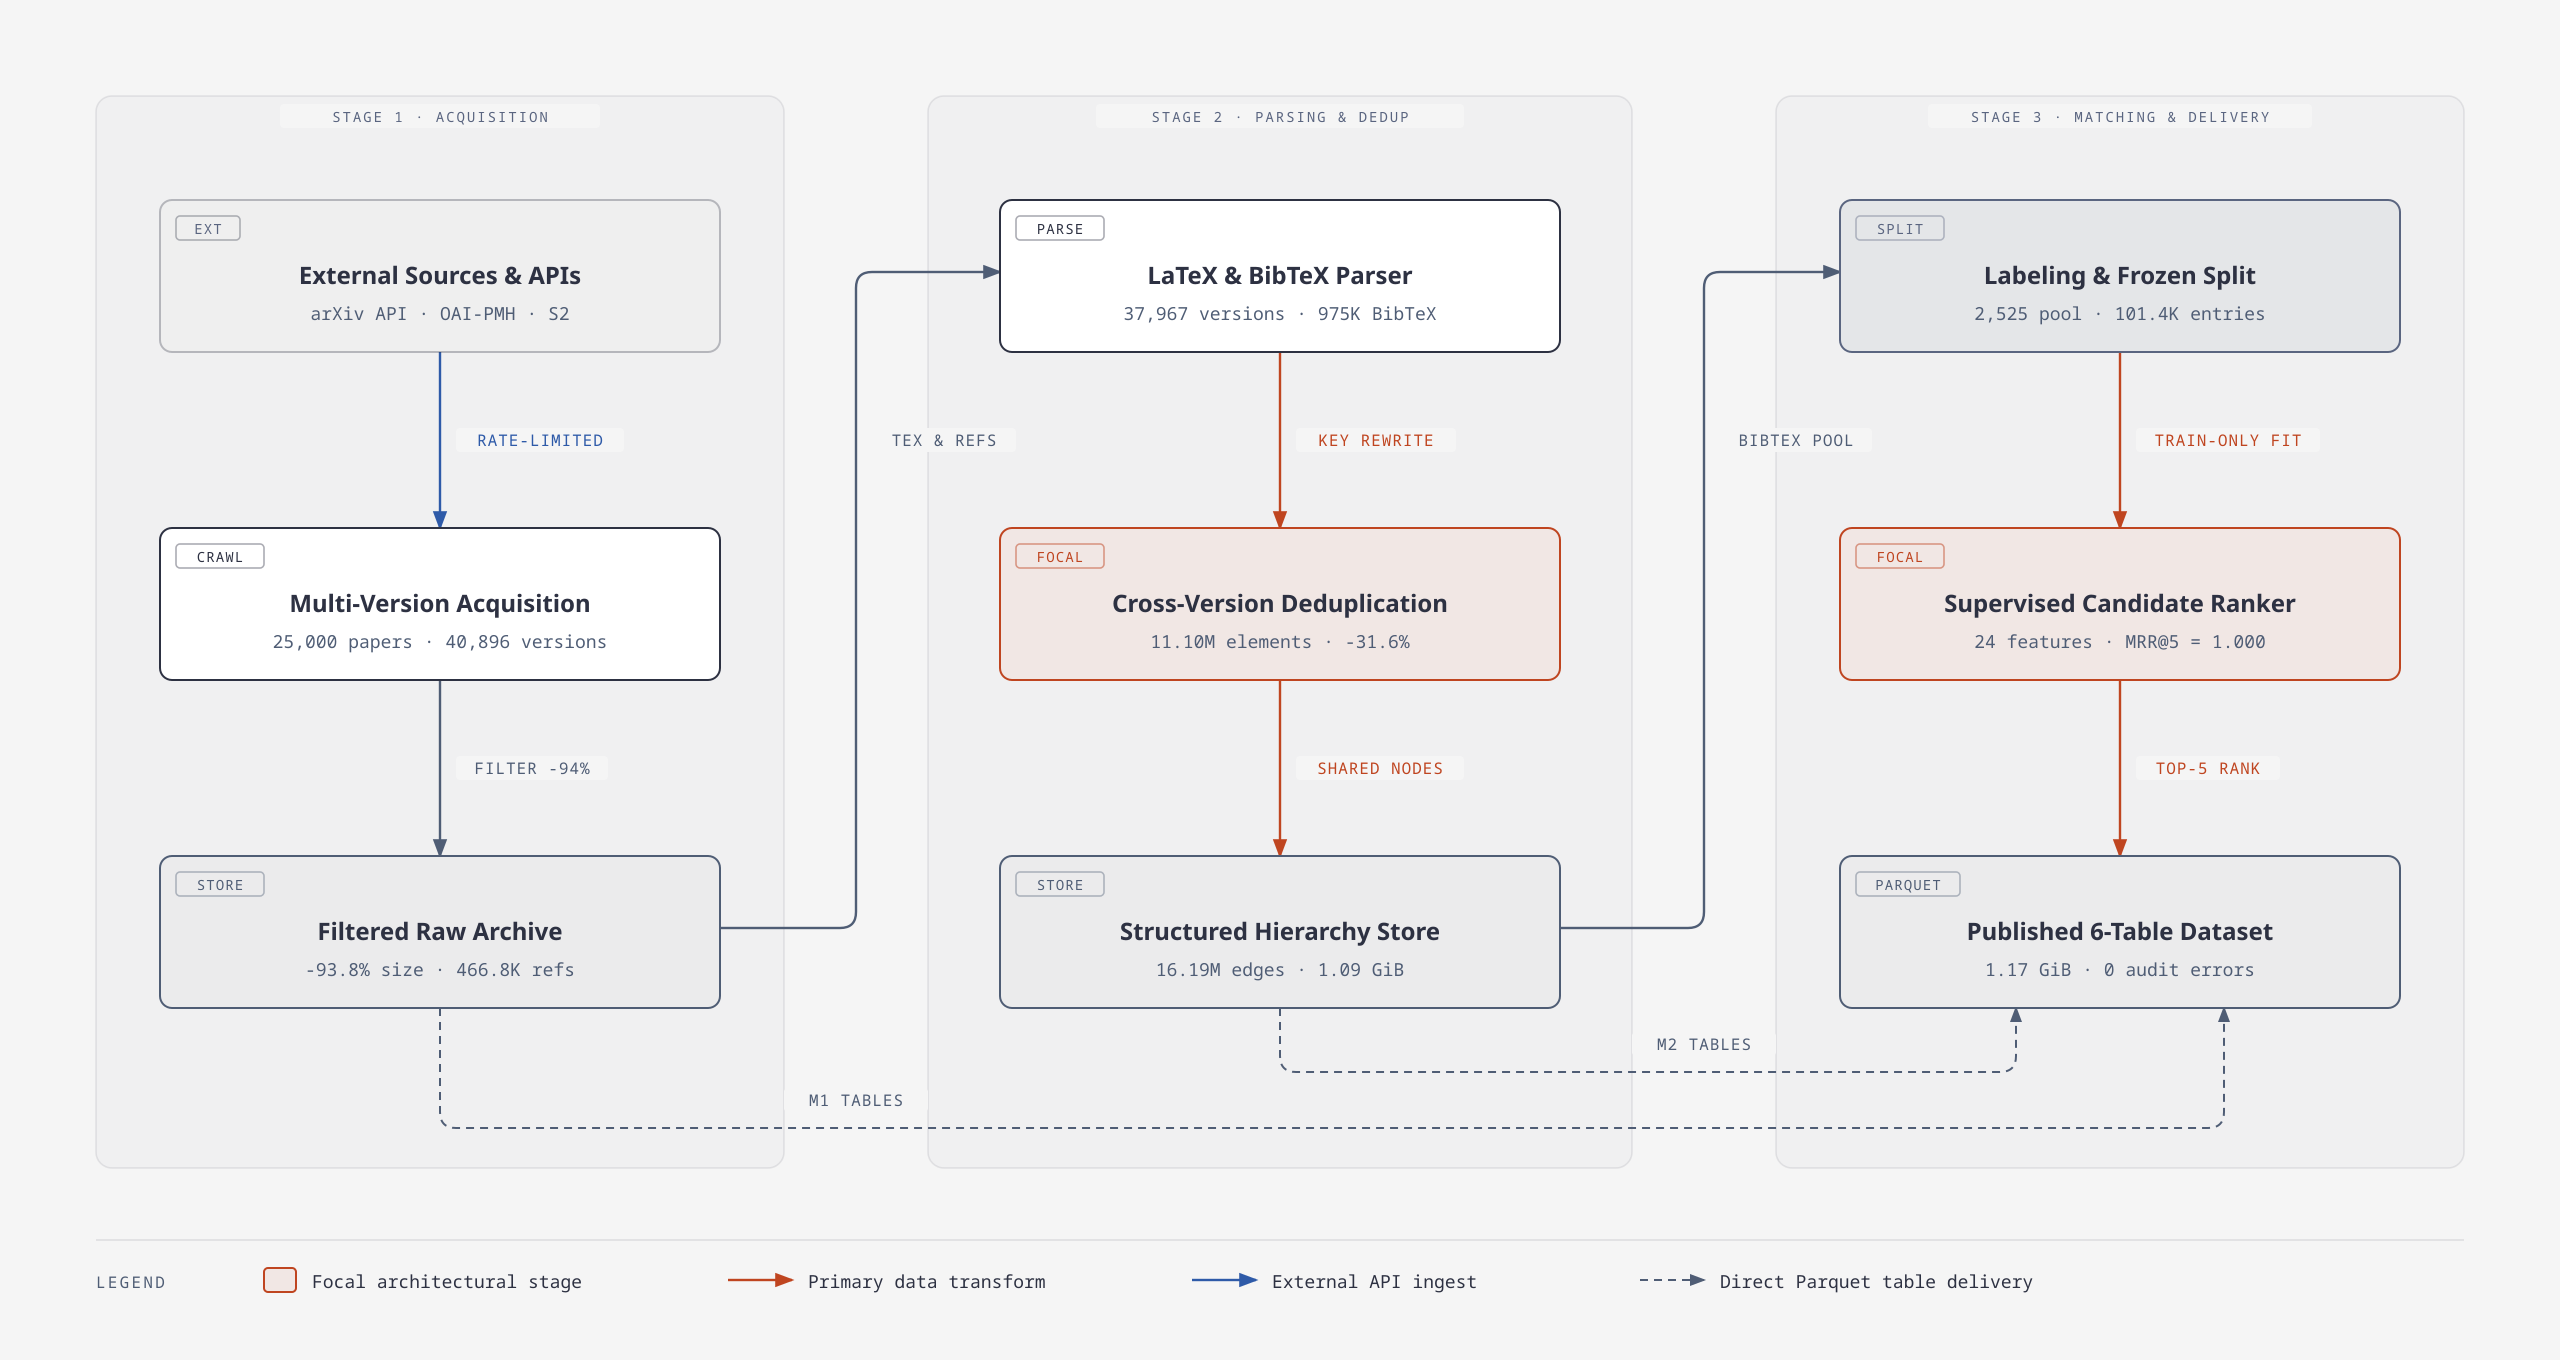
\includegraphics[width=\linewidth]{images/e2e_architecture.png}
    \caption[Kiến trúc tổng thể ba giai đoạn của hệ thống xử lý kho bài báo arXiv]{Kiến trúc tổng thể ba giai đoạn của hệ thống khai thác, phân tích phân cấp và đối sánh tài liệu tham khảo trên kho $25{,}000$ bài báo arXiv, nhấn mạnh ranh giới cách ly hợp đồng dữ liệu, cơ chế vận hành thuần CPU và sáu bảng xuất bản định dạng cột Parquet.}
    \label{fig:e2e_architecture}
\end{figure}

Hai nguyên tắc kỹ thuật xuyên suốt toàn bộ kiến trúc là tính tuân thủ học thuật tuyệt đối về không sử dụng tri thức tiền huấn luyện bên ngoài và khả năng tái lập hoàn toàn trên phần cứng CPU phổ thông~\cite{hcmus_intro_ds}. Hệ thống không gọi bất kỳ mô hình ngôn ngữ lớn, vectơ nhúng ngữ nghĩa tiền huấn luyện hay dịch vụ suy luận ngoài nào trong các khâu chuẩn hóa văn bản, gán nhãn, rút trích đặc trưng và huấn luyện mô hình đối sánh; toàn bộ từ điển n-gram ký tự TF-IDF, hệ số chuẩn hóa và tham số mô hình học có giám sát đều được ước lượng hoàn toàn bên trong tập huấn luyện với hạt giống ngẫu nhiên cố định. Về mặt hạ tầng tính toán, các công đoạn nặng về mạng và nhập xuất được thiết kế chịu lỗi trên máy ảo đám mây Google Colab có tài nguyên khiêm tốn ($2$ vCPU và khoảng $12.68\text{ GiB}$ RAM), trong khi toàn bộ lượt huấn luyện, kiểm định chéo năm phần và suy luận Giai đoạn 3 cho cả năm thành viên chỉ tiêu tốn $12.88\text{ phút}$ trên $2$ luồng CPU với đỉnh bộ nhớ $2{,}393.5\text{ MB}$. Ở tầng lưu trữ phát hành, thay vì duy trì hàng trăm nghìn tệp văn bản rời rạc gây nghẽn hệ thống tệp, toàn bộ kết quả ba giai đoạn được hợp nhất thành sáu bảng dữ liệu phân mảnh theo định dạng lưu trữ cột Apache Parquet~\cite{apache_parquet}. Cơ chế nén theo cột kết hợp mã hóa từ điển giúp toàn bộ kho dữ liệu $25{,}000$ bài báo đa phiên bản (bao gồm hơn $11$ triệu phần tử nội dung và hơn $16$ triệu cạnh phân cấp) chỉ chiếm đúng $1{,}199.45\text{ MiB}$ ($1.171\text{ GiB}$), đồng thời hỗ trợ truy vấn chọn lọc cột trực tiếp mà không cần giải nén toàn bộ bảng vào bộ nhớ chính.

\begin{figure}[htbp]
    \centering
    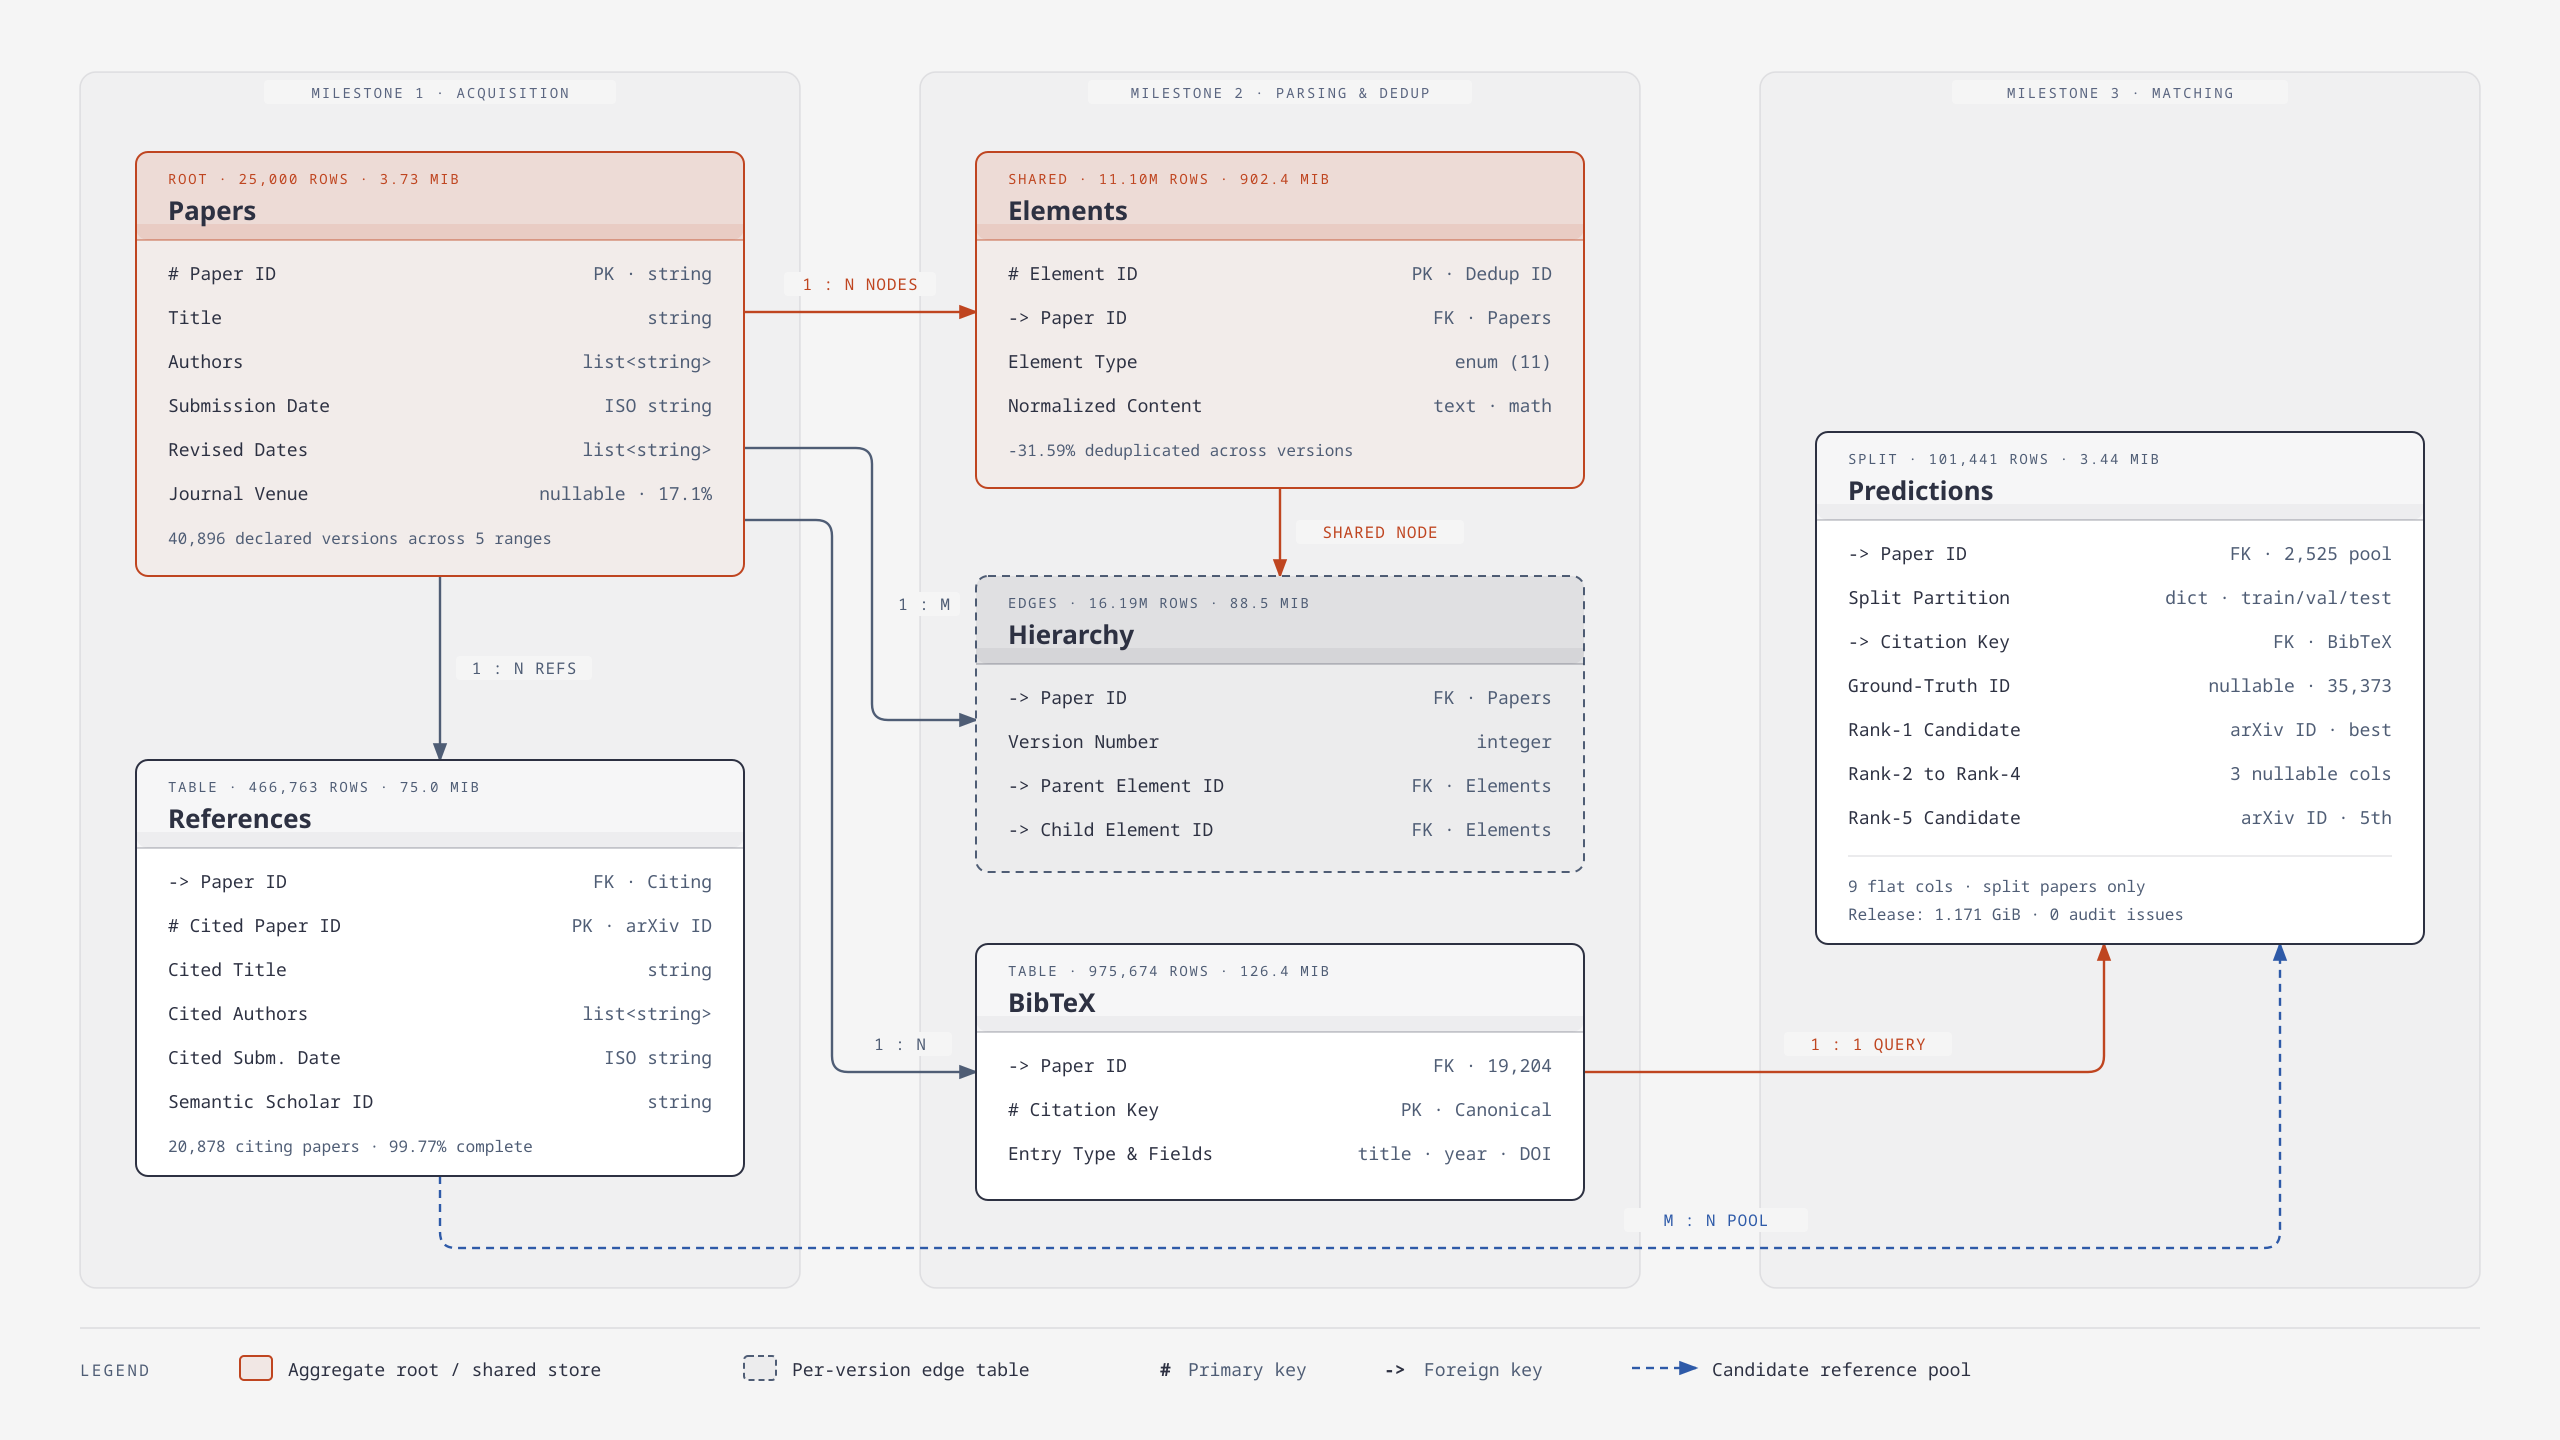
\includegraphics[width=\linewidth]{images/data_schema_er.png}
    \caption[Mô hình thực thể -- liên kết sáu bảng dữ liệu cột Apache Parquet]{Mô hình thực thể -- liên kết chuẩn hóa gồm sáu bảng dữ liệu cột Apache Parquet xoay quanh khóa mã định danh arXiv không phiên bản, tách biệt kho phần tử nội dung đã khử trùng lặp khỏi bảng cạnh quan hệ phân cấp theo từng phiên bản.}
    \label{fig:data_schema_er}
\end{figure}

Cấu trúc quan hệ giữa sáu bảng phát hành được trình bày trực quan tại Hình~\ref{fig:data_schema_er} và đặc tả khái niệm chi tiết trong Bảng~\ref{tab:six_tables}. Toàn bộ lược đồ xoay quanh khóa định danh bài báo arXiv chuẩn hóa không mang hậu tố phiên bản, bảo đảm mọi thực thể từ siêu dữ liệu bài báo, tài liệu tham khảo bên ngoài, cây văn bản đa phiên bản đến kết quả đối sánh đều nối kết nhất quán qua một trục khóa duy nhất. Quyết định chuẩn hóa mang tính nền tảng của mô hình dữ liệu nằm ở việc tách rời bảng phần tử nội dung duy nhất khỏi bảng quan hệ phân cấp theo từng phiên bản: một câu văn hoặc công thức toán học giữ nguyên qua các phiên bản $v_1, v_2, \dots, v_k$ chỉ lưu trữ nguyên văn đúng một lần trong bảng phần tử, trong khi bảng quan hệ phân cấp dùng các bộ khóa nhẹ chỉ mục phiên bản, nút cha và nút con để tái tạo nguyên vẹn cấu trúc cây có thứ tự của từng phiên bản riêng biệt. Tương tự, việc tách biệt bảng mục lục BibTeX khai báo bên trong bài báo với bảng tài liệu tham khảo thu hoạch từ Semantic Scholar giúp phân tách rõ ràng giữa phát biểu trích dẫn của tác giả và tập ứng viên đích ngoài đồ thị tri thức cho đến khi bảng kết quả dự đoán đối sánh liên kết hai phía ở Giai đoạn 3. Trước khi đóng gói phát hành cuối cùng, toàn bộ năm phân mảnh thành viên của cả sáu bảng đều vượt qua quy trình kiểm định tự động về khóa chính, toàn vẹn khóa ngoại và định dạng dữ liệu với kết quả $0$ lỗi phát sinh.

\begin{table}[htbp]
    \centering
    \scriptsize
    \setlength{\tabcolsep}{4pt}
    \renewcommand{\arraystretch}{1.24}
    \begin{tabularx}{\textwidth}{p{0.19\textwidth} c p{0.21\textwidth} X r r}
        \toprule
        \textbf{Bảng dữ liệu} & \textbf{GĐ} & \textbf{Khóa logic \& Quan hệ} & \textbf{Vai trò khái niệm trong kho dữ liệu} & \textbf{Số dòng} & \textbf{Parquet} \\
        \midrule
        Bảng siêu dữ liệu bài báo & GĐ 1 & Khóa chính: mã arXiv không phiên bản (bảng trung tâm $1$) & Lưu tiêu đề, tác giả chuẩn hóa, chuỗi ngày nộp và hiệu chỉnh đầy đủ $v_1 \dots v_N$, nơi công bố chính thức và phạm vi sở hữu. & 25,000 & 3.73 MiB \\
        Bảng tài liệu tham khảo & GĐ 1 & Khóa ghép: mã bài trích dẫn + mã arXiv đích ($1:N$ từ bài báo) & Lưu danh mục bài báo arXiv được trích dẫn thu từ Semantic Scholar kèm tiêu đề, tác giả và ngày nộp $v_1$ chuẩn hóa từ arXiv. & 466,763 & 75.01 MiB \\
        Bảng phần tử nội dung & GĐ 2 & Khóa ghép: mã bài báo + mã phần tử duy nhất ($1:N$ từ bài báo) & Lưu kho văn bản sạch đã khử trùng lặp liên phiên bản cho từng loại nút cấu trúc (mục, câu văn, công thức khối, hình bảng, danh sách). & 11,098,189 & 902.35 MiB \\
        Bảng quan hệ phân cấp & GĐ 2 & Khóa ghép: mã bài báo + phiên bản + nút cha + nút con ($N:M$) & Tái tạo trọn vẹn cây cấu trúc có thứ tự của từng phiên bản bằng cách liên kết các nút thuộc bảng phần tử nội dung. & 16,185,255 & 88.50 MiB \\
        Bảng mục lục BibTeX & GĐ 2 & Khóa ghép: mã bài báo + khóa trích dẫn hợp nhất ($1:N$ từ bài báo) & Hợp nhất các mục thư mục từ nguồn BibTeX và mục tham khảo nội tuyến xuyên phiên bản gồm tiêu đề, tác giả, năm, tạp chí, DOI và liên kết. & 975,674 & 126.41 MiB \\
        Bảng kết quả dự đoán đối sánh & GĐ 3 & Khóa ghép: mã bài báo + khóa trích dẫn mẫu ($1:1$ trên tập mẫu) & Lưu phân hoạch tập dữ liệu, nhãn đối sánh, mã arXiv chuẩn đối chiếu và danh sách năm ứng viên xếp hạng cao nhất của mô hình. & 101,441 & 3.44 MiB \\
        \midrule
        \textbf{Tổng hợp 6 bảng} & \textbf{GĐ 1--3} & \textbf{5 phân mảnh thành viên, 0 lỗi kiểm định toàn vẹn} & \textbf{Kho dữ liệu cột hợp nhất cho toàn bộ $25{,}000$ bài báo chính thức (tương đương $1.171\text{ GiB}$).} & \textbf{28,852,322} & \textbf{1,199.45 MiB} \\
        \bottomrule
    \end{tabularx}
    \caption[Đặc tả khái niệm sáu bảng dữ liệu xuất bản Apache Parquet]{Đặc tả khái niệm sáu bảng dữ liệu chuẩn hóa được xuất bản dưới định dạng lưu trữ cột Apache Parquet cho toàn nhóm ChickenDev. Tổng dung lượng $1{,}199.45\text{ MiB}$ ($1.171\text{ GiB}$) là tổng chính xác trước khi làm tròn hai chữ số thập phân ở từng bảng.}
    \label{tab:six_tables}
\end{table}

\section{Giai đoạn 1: Thu thập dữ liệu đa nguồn và tối ưu lưu trữ}

\subsection{Chiến lược dò tìm bài báo và thu hoạch lịch sử phiên bản}

Bài toán xác định trọn vẹn tập bài báo hợp lệ trong mỗi dải mã arXiv được giao không đơn thuần là phép tăng số tuần tự, đặc biệt khi dải mã bắc ngang ranh giới hai tháng dương lịch. Theo quy ước định danh của arXiv, bộ đếm năm chữ số sẽ đặt lại về $00001$ vào ngày đầu mỗi tháng trong khi ngưỡng số thứ tự cuối cùng của tháng trước đó không cố định và không có giao diện tra cứu trực tiếp~\cite{arxiv_api}. Thay vì ước đoán ngưỡng kết thúc tháng hoặc dừng sớm khi gặp một vài khe mã bị rút bài, phân hệ dò tìm tạo danh sách ứng viên theo từng lô $100$ mã và quét cạn tới $99{,}999$ của tháng mở đầu trước khi chuyển sang $00001$ của tháng kế tiếp. Chính cơ chế quét an toàn này giải thích vì sao hai dải xuyên tháng phải kiểm định $83{,}142$ mã (từ $2504.17523$ đến $2504.99999$ cộng $665$ mã tháng $05/2025$) và $80{,}870$ mã (từ $2506.20788$ đến $2506.99999$ cộng $1{,}658$ mã tháng $07/2025$) thay vì đúng $5{,}000$ mã như ba dải nội tháng. Mọi truy vấn gửi tới cổng tìm kiếm Atom của arXiv đều tuân thủ nghiêm ngặt quy tắc một kết nối đơn với khoảng nghỉ tối thiểu $3\text{ giây}$ giữa hai lần gọi~\cite{arxiv_api}. Nhằm ngăn ngừa kết luận sai rằng bài báo không tồn tại khi máy chủ trả phản hồi cắt xén, bộ phân tích chỉ chấp nhận suy diễn vắng mặt khi thỏa đồng thời bất biến đầy đủ phân trang: chỉ số khởi đầu phản hồi bằng $0$ và tổng số kết quả khai báo trùng khớp tuyệt đối với số mục thực nhận trong tài liệu XML. Bất cứ lô truy vấn nào xuất hiện sai lệch số lượng, thiếu thẻ phân trang hoặc cấu trúc bất thường đều tự động chuyển sang chế độ truy vấn đơn lẻ cho từng mã ứng viên, đồng thời áp đặt giới hạn kích thước gói phản hồi và vô hiệu hóa cơ chế mở rộng thực thể XML ngoài nhằm phòng ngừa tấn công tiêm thực thể và tràn bộ nhớ.

Mặc dù giao diện Atom đáp ứng tốt bài toán phát hiện sự tồn tại của bài báo, dịch vụ này chỉ công bố hai mốc thời gian là ngày nộp đầu tiên và ngày cập nhật gần nhất, làm thất lạc hoàn toàn lịch sử các phiên bản trung gian $v_2, \dots, v_{N-1}$. Trong kho dữ liệu thực tế của nhóm, có tới $42.64\%$ bài báo sở hữu từ hai phiên bản trở lên (tối đa tới $v_{13}$), khiến việc dùng Atom cho thu hoạch siêu dữ liệu trở nên bất khả thi đối với yêu cầu bảo toàn nguồn gốc thời gian ở mức phiên bản. Do đó, hệ thống chuyển công đoạn thu hoạch siêu dữ liệu sang giao thức OAI-PMH trên điểm cuối đám mây mới mà arXiv chính thức di chuyển từ tháng $03/2025$~\cite{arxiv_oai_2025}, sử dụng định dạng siêu dữ liệu gốc đầy đủ của arXiv để lấy đồng thời danh sách trọn vẹn từng phiên bản kèm dấu thời gian chính xác và thông tin nơi công bố chính thức. Do chuỗi danh sách tác giả thô trên arXiv thường trộn lẫn tên đơn vị công tác trong dấu ngoặc đơn, cụm dấu ngoặc nhọn chứa dấu phụ LaTeX, hậu tố thế hệ sau dấu phẩy và tên tổ hợp nghiên cứu, bộ chuẩn hóa tác giả tất định thực hiện tách theo nhiều bước: loại bỏ chú thích đơn vị trong ngoặc đơn, bảo toàn khối ngoặc nhọn cân bằng khi tách dấu phẩy, gắn lại hậu tố thế hệ vào họ tác giả liền trước và tách riêng tiền tố nhóm hợp tác. Toàn bộ mốc thời gian thu nhận từ cả OAI-PMH lẫn Atom đều được quy đổi về định dạng chuẩn giờ phối hợp quốc tế UTC có gắn thông tin múi giờ nhằm loại trừ sai lệch đồng hồ cục bộ khi đối chiếu chuỗi phiên bản và ngày trích dẫn về sau.

\subsection{Tải mã nguồn toàn văn đa định dạng và lọc bỏ tài nguyên nhị phân}

Công đoạn tải toàn văn mã nguồn cho từng phiên bản bài báo được định tuyến tuyệt đối về máy chủ gương xuất dữ liệu chuyên dụng của arXiv thay vì truy cập cổng web công cộng, kèm theo tiêu đề định danh tác nhân khách mô tả rõ danh tính học thuật và chu kỳ giãn cách $3\text{ giây}$ nhằm tôn trọng chính sách tải hàng loạt~\cite{arxiv_api}. Mỗi phiên tải áp đặt kiểm tra mã trạng thái HTTP $200$ trọn vẹn, từ chối rõ ràng các phản hồi phân đoạn HTTP $206$ vốn có thể âm thầm cắt cụt dòng nén, đồng thời duy trì ngưỡng giới hạn dung lượng đọc luồng để tránh làm kiệt quệ bộ nhớ máy ảo trước các gói nén dị thường. Do điểm cuối xuất mã nguồn của arXiv phục vụ nhiều định dạng nộp bài khác nhau dưới cùng một cấu trúc đường dẫn mà không bảo đảm độ tin cậy của tiêu đề kiểu nội dung, tầng tiếp nhận không dựa vào đuôi tên tệp mà thực hiện nhận diện chữ ký byte mở đầu kết hợp kiểm tra tiêu đề cấu trúc tệp. Cơ chế nhận diện đa tầng này phân loại chính xác mọi gói tải về vào sáu nhóm định dạng thực tế: gói nén tar dùng thuật toán gzip, gói tar không nén, tệp văn bản TeX nén đơn bằng gzip, tệp văn bản TeX thuần không nén, bài nộp chỉ gồm tài liệu PDF và tài liệu soạn thảo theo chuẩn Office Open XML. Nhờ tách biệt việc nhận diện nhị phân khỏi phần mở rộng đường dẫn, bộ tiếp nhận xử lý an toàn cả các luồng nén lồng nhau lẫn tệp văn bản thuần bị gắn nhãn nén sai lệch. Quy trình phối hợp giữa dò tìm, thu hoạch siêu dữ liệu, nhận diện định dạng, lọc nguồn và xuất bản nguyên tử được tổng hợp trực quan trong Hình~\ref{fig:m1_crawling_flow}.

\begin{figure}[htbp]
    \centering
    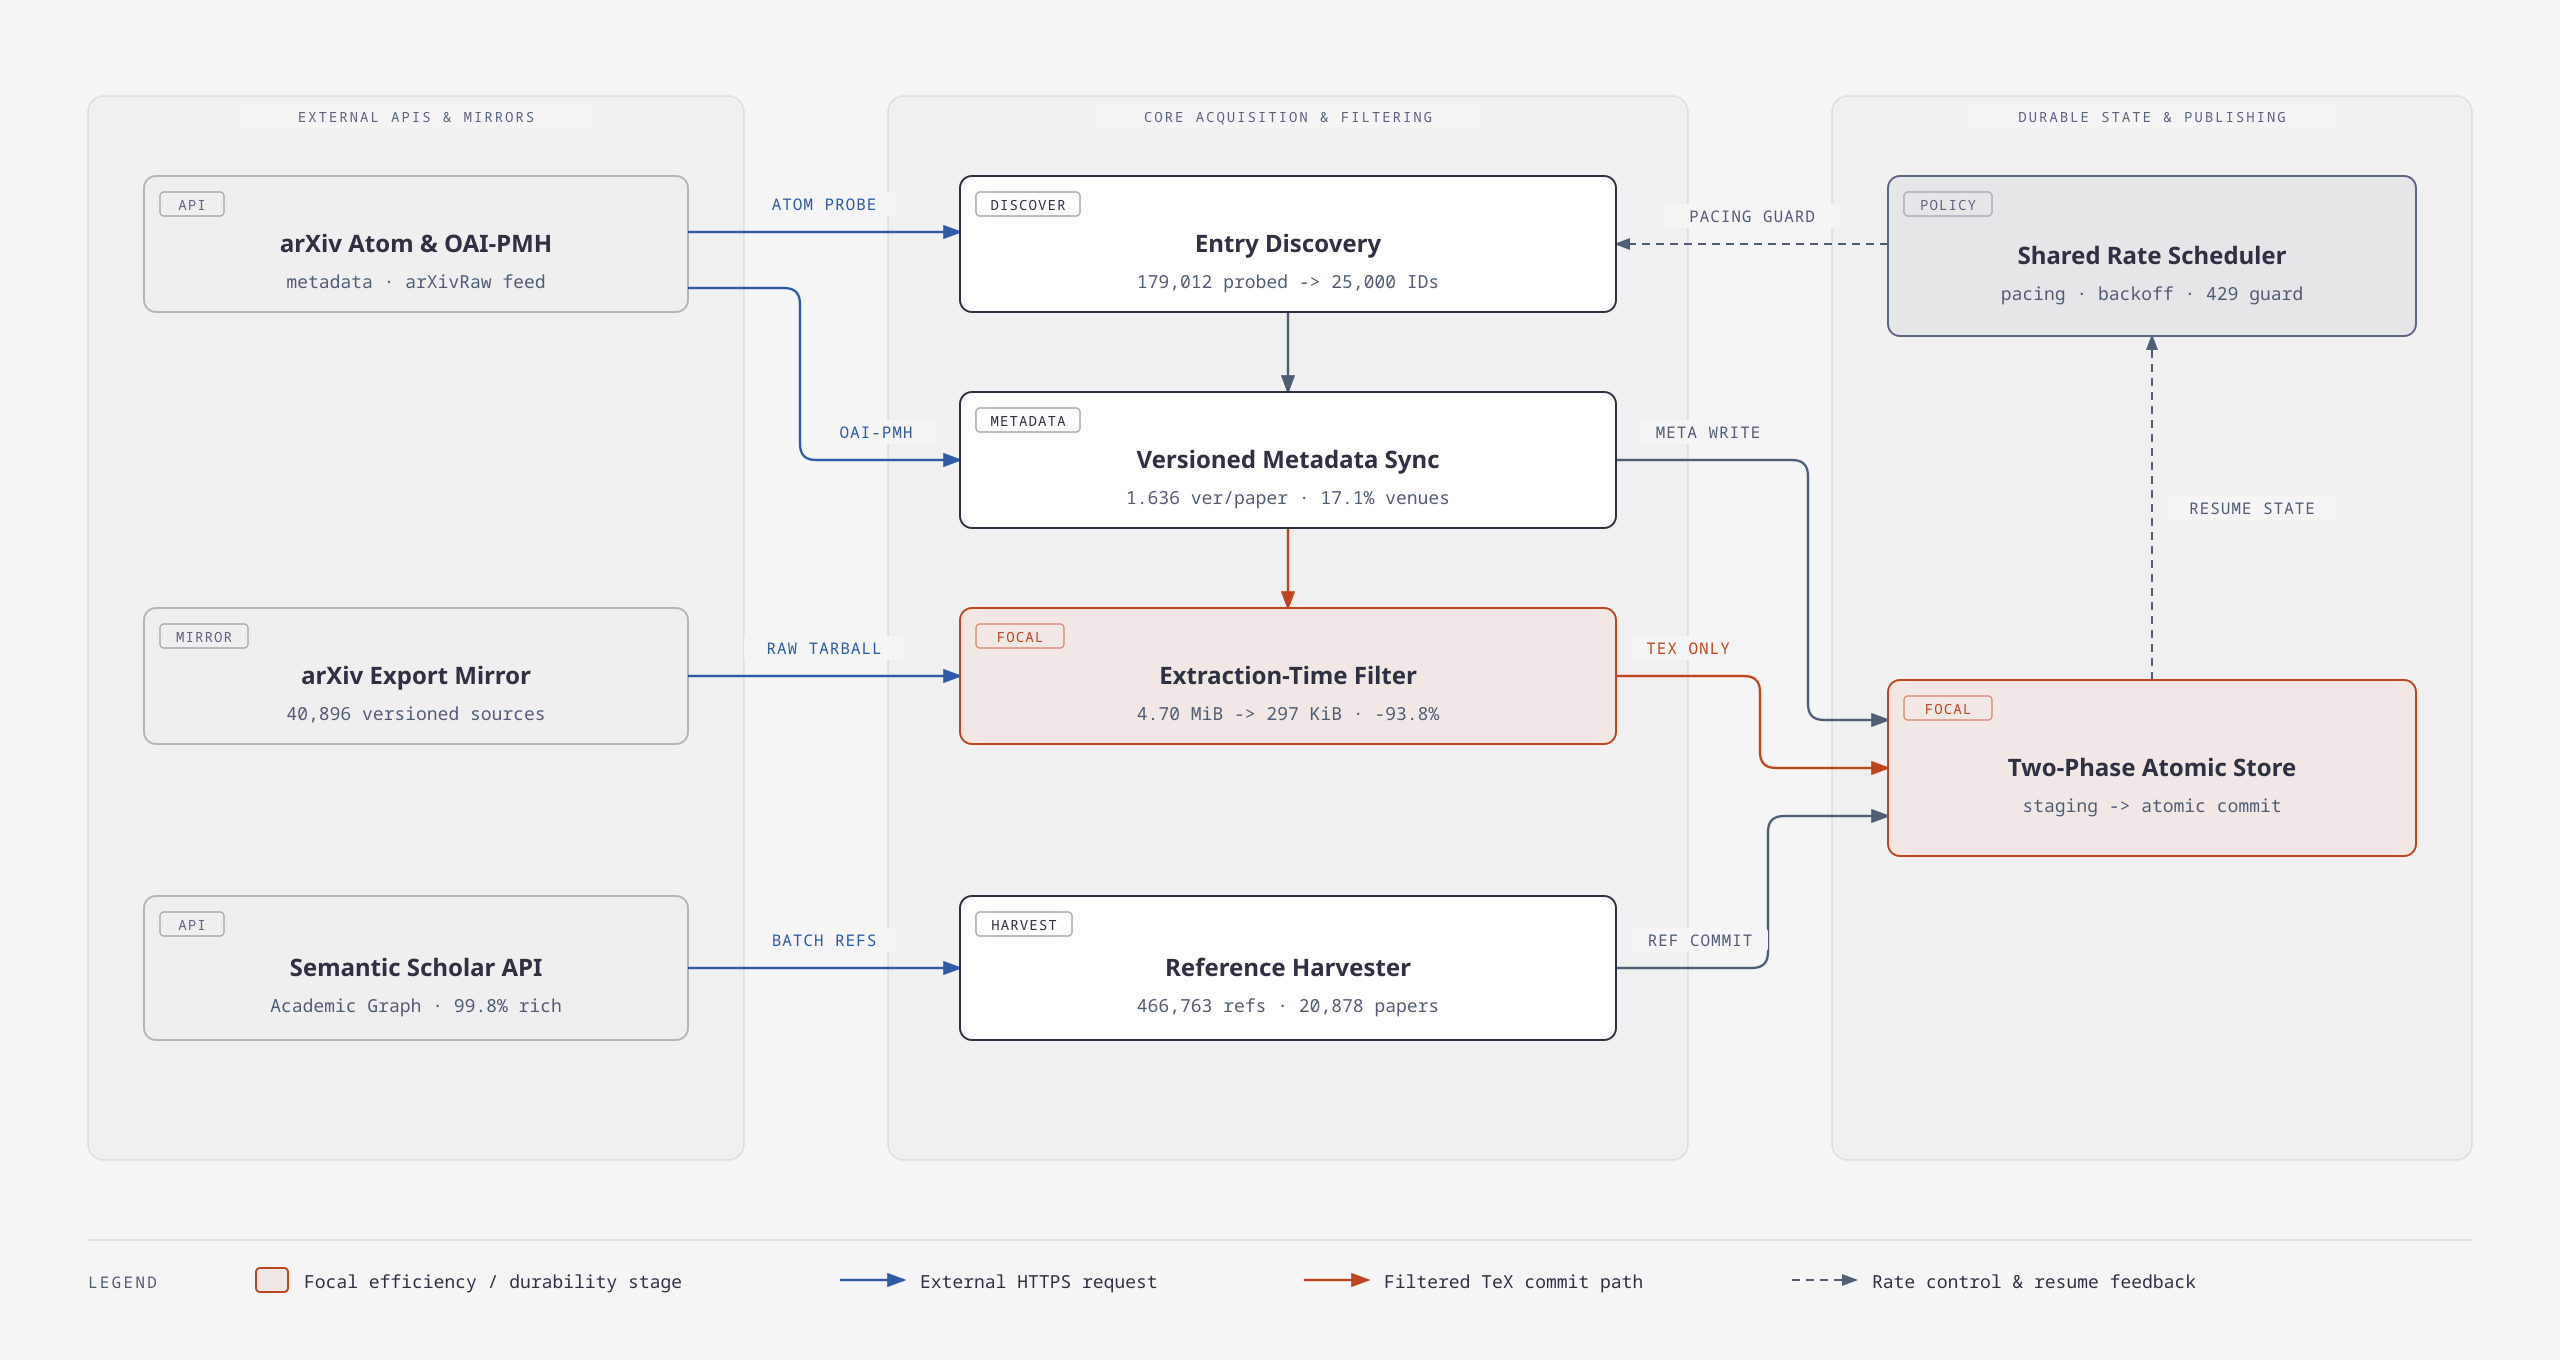
\includegraphics[width=\linewidth]{images/m1_crawling_flow.png}
    \caption[Quy trình thu thập dữ liệu đa nguồn và tối ưu lưu trữ ở Giai đoạn 1]{Quy trình thu thập dữ liệu đa nguồn và tối ưu lưu trữ ở Giai đoạn 1: dò tìm lô xuyên ranh giới tháng, thu hoạch lịch sử phiên bản OAI-PMH, nhận diện sáu định dạng và lọc chọn lọc ngay lúc giải nén, thu hoạch mạng trích dẫn Semantic Scholar có khắc phục lỗi tiêu đề khóa API và xuất bản giao dịch hai pha.}
    \label{fig:m1_crawling_flow}
\end{figure}

Phần lớn dung lượng của một gói mã nguồn bài báo khoa học trên arXiv đến từ hình ảnh độ phân giải cao, đồ thị vectơ và các tệp dữ liệu nhị phân phụ trợ. Nếu lưu nguyên trạng toàn bộ $40{,}896$ phiên bản, kho lưu trữ sẽ tiêu tốn xấp xỉ $200\text{ GiB}$ và nhanh chóng vượt quá dung lượng của môi trường đám mây phổ thông. Để giải quyết triệt để nút thắt lưu trữ mà không ảnh hưởng đến tính nguyên vẹn văn bản, bộ lọc hoạt động trực tiếp tại thời điểm giải nén và chỉ giữ lại nguyên vẹn từng byte các tệp mã nguồn TeX cùng tệp thư mục BibTeX, tuyệt đối không chỉnh sửa hay xóa bỏ các lệnh chèn hình ảnh hoặc bảng biểu bên trong mã TeX để bảo toàn nguyên trạng ngữ cảnh phân tích cho Giai đoạn 2. Trước khi giải nén bất kỳ thành phần nào trong gói lưu trữ, hàng rào bảo mật sẽ từ chối liên kết mềm, liên kết cứng, đường dẫn tuyệt đối và chuỗi vượt cấp thư mục cha, kiểm định mã kiểm tra vòng CRC ở phần đuôi dòng gzip chống lỗi hỏng dữ liệu, đồng thời giới hạn số lượng tệp cùng tổng kích thước bung nén nhằm vô hiệu hóa nguy cơ bom giải nén. Với mọi phiên bản có mã nguồn hợp lệ, quá trình lọc phải thỏa mãn bất biến hạch toán dung lượng chính xác tại Phương trình~\eqref{eq:m1_byte_accounting} giữa tổng kích thước gói tải về $B_{\text{raw}}$, dung lượng mã nguồn giữ lại $B_{\text{src}}$, dung lượng tài nguyên nhị phân loại bỏ $B_{\text{bin}}$ và phần phụ trội cấu trúc gói nén $B_{\text{ovh}}$:
\begin{equation}
    B_{\text{raw}} = B_{\text{src}} + B_{\text{bin}} + B_{\text{ovh}}, \qquad
    \rho_{\text{save}} = 1 - \frac{B_{\text{src}}}{B_{\text{raw}}}.
    \label{eq:m1_byte_accounting}
\end{equation}
Đối với khoảng $5.38\%$ đến $7.28\%$ phiên bản không chứa mã nguồn TeX (chủ yếu là bài nộp PDF thuần hoặc tài liệu Office Open XML, nhất quán với mức bao phủ nguồn TeX khoảng $97\%$ cùng tỷ lệ ngoại lệ trên toàn kho arXiv~\cite{ginev2024}), hệ thống kiên quyết không xóa bỏ bài báo mà vẫn ghi nhận hồ sơ nguồn rỗng có đánh dấu trạng thái rõ ràng nhằm giữ vẹn toàn tập hợp $25{,}000$ bài báo chính thức xuyên suốt mọi bảng thống kê.

\subsection{Khai thác mạng lưới trích dẫn, khắc phục giới hạn tần suất và cơ chế bền vững}

Để tạo tập ứng viên tài liệu tham khảo đầu vào cho bài toán đối sánh có giám sát ở Giai đoạn 3, phân hệ thu thập trích dẫn tích hợp với giao diện lập trình đồ thị học thuật của Semantic Scholar~\cite{kinney2023}, nền tảng đạt độ chính xác trích xuất tài liệu tham khảo trên $90\%$ trong xây dựng đồ thị văn học khoa học~\cite{ammar2018}. Các truy vấn chỉ yêu cầu tập trường thư mục dạng phẳng nhằm thu gọn băng thông truyền tải trong khi vẫn lưu trữ đầy đủ toàn bộ danh sách trích dẫn thô tại kho cục bộ để phục vụ đối chiếu kiểm toán khi cần thiết. Khi xuất bản dữ liệu cho giai đoạn đối sánh, hệ thống lọc lấy các tài liệu tham khảo sở hữu mã định danh ngoài của arXiv, bảo toàn cẩn trọng cả định dạng số mới lẫn định dạng tiền năm $2007$ có tiền tố lĩnh vực kèm dấu gạch chéo ($\text{lĩnh vực}/\text{YYMMNNN}$). Một sai lệch ngữ nghĩa nghiêm trọng thường gặp ở bước này là trường ngày công bố trên Semantic Scholar thường phản ánh ngày xuất bản tại tạp chí hoặc hội nghị (có thể trễ hơn bản tiền ấn phẩm từ một đến ba năm), trong khi yêu cầu bài toán đòi hỏi chính xác ngày nộp phiên bản đầu tiên $v_1$ trên arXiv. Nhằm đáp ứng đúng hợp đồng dữ liệu mà không lặp lại truy vấn mạng thừa thãi, bộ thu thập tổng hợp tất cả mã arXiv được trích dẫn duy nhất trên toàn bộ tập bài báo rồi thực hiện tra cứu theo lô đã khử trùng lặp trực tiếp từ arXiv để giải mã ngày nộp $v_1$ một lần duy nhất và ánh xạ đồng bộ về mọi bài báo trích dẫn liên quan.

Trong quá trình mở rộng quy mô thu hoạch trên Semantic Scholar, hệ thống ghi nhận một sự cố kỹ thuật đáng chú ý khi các yêu cầu đã gắn khóa API hợp lệ vẫn liên tục nhận mã lỗi giới hạn tần suất HTTP $429$ tương ứng với hạn mức công khai không xác thực. Phân tích sâu ở tầng giao thức truyền tải cho thấy các thư viện khách HTTP bậc cao phổ biến mặc định tự động chuẩn hóa tên trường tiêu đề yêu cầu theo kiểu viết hoa chữ cái đầu mỗi từ. Tuy nhiên, cổng biên của dịch vụ đích chỉ nhận diện trường tiêu đề khóa API ở dạng chữ thường thuần túy, dẫn tới việc khóa xác thực bị bỏ qua âm thầm và toàn bộ lưu lượng bị hạ bậc xuống hạn mức công khai dùng chung. Vấn đề được xử lý dứt điểm bằng cách triển khai một tầng kết nối TLS HTTP/1.1 trực tiếp cho luồng gọi có xác thực, bảo toàn nguyên trạng chữ thường của tiêu đề khóa API khi tuần tự hóa gói tin và lập tức khôi phục trọn vẹn băng thông định mức đã cấp. Song hành với bản vá giao thức này, tầng truyền tải chủ động vô hiệu hóa hoàn toàn cơ chế tự động chuyển hướng sang máy chủ khác tên miền trên các kết nối có đính kèm khóa API, ngăn chặn tuyệt đối rủi ro rò rỉ thông tin xác thực qua phản hồi chuyển hướng HTTP.

Vì mỗi dải $5{,}000$ bài báo đòi hỏi hơn một ngày thu thập liên tục trong điều kiện phiên chạy đám mây Google Colab có thể ngắt kết nối đột ngột sau ngưỡng nhàn rỗi hoặc giới hạn thời lượng phiên, tính bền vững và khả năng phục hồi tức thì là điều kiện tiên quyết của thiết kế vận hành. Bộ điều phối tần suất bền vững đồng thời cưỡng chế khoảng giãn cách $3\text{ giây}$ cho arXiv cùng ràng buộc kép trên Semantic Scholar gồm nhịp duy trì $1\text{ yêu cầu/giây}$ kết hợp cửa sổ trượt $100\text{ yêu cầu mỗi } 5\text{ phút}$, đi kèm cơ chế lùi thời gian theo hàm mũ có nhiễu ngẫu nhiên khi gặp lỗi máy chủ tạm thời hoặc mã HTTP $429$. Đối với bước thu hoạch trích dẫn, hệ thống sử dụng các yêu cầu gửi hàng loạt theo lô thích ứng để giảm thiểu độ trễ mạng. Bất cứ khi nào một lô lớn bị quá thời gian chờ hoặc trả lỗi cục bộ, bộ lập lịch sẽ tự động chia đôi đệ quy kích thước lô xuống tới mức đơn lẻ nhằm cô lập mã bài báo bất thường mà không làm đình trệ toàn lô. Trạng thái hoàn thành chi tiết tới từng công đoạn bài báo được cập nhật bền vững trong cơ sở dữ liệu quan hệ nhúng SQLite, cho phép nối tiếp phiên chạy sau hàng chục lần khởi động lại mà không tải lặp dữ liệu cũ. Cuối cùng, khâu đưa dữ liệu đã xử lý vào vùng lưu trữ chính thức tuân theo giao thức xuất bản giao dịch hai pha: toàn bộ tệp đầu ra được ghi vào vùng đệm cô lập kèm tính toán mã băm toàn vẹn SHA-256 cho từng tệp, và chỉ sau khi xác thực trọn vẹn hệ thống mới thực hiện chuyển đổi nguyên tử bảng kê dữ liệu sang trạng thái hoạt động, kết hợp cơ chế tự phục hồi mỗi khi khởi động lại để dọn dẹp hoặc hoàn tất mọi giao dịch bị ngắt ngang giữa chừng.

\subsection{Kết quả thống kê kho dữ liệu và đo lường hiệu năng trên Google Colab CPU}

Để bảo đảm tính trung thực thực nghiệm cao nhất, kết quả định lượng của Giai đoạn 1 được báo cáo tách bạch rõ ràng giữa hai tập số liệu: kho dữ liệu chính thức hoàn chỉnh gồm $25{,}000$ bài báo sau khi hội tụ đầy đủ mọi đợt thu hoạch và bù trích dẫn (Bảng~\ref{tab:m1_final_corpus}), và bản chụp đo lường hiệu năng phần cứng cùng hiệu quả lọc mã nguồn trên Google Colab tại thời điểm bàn giao ngày $06/11/2026$ (Bảng~\ref{tab:m1_benchmark}). Trên kho dữ liệu hoàn chỉnh gồm $25{,}000$ bài báo, hệ thống đã thu hoạch chính xác $40{,}896$ phiên bản khai báo, đạt trung bình $1.636$ phiên bản mỗi bài và phân bố rất đồng đều giữa năm dải từ $1.587$ đến $1.677$. Xét theo phân bố số lượng phiên bản, bài báo đơn phiên bản ($v_1$) chiếm $14{,}341$ bài ($57.36\%$), trong khi nhóm bài báo đa phiên bản ($\ge 2$ phiên bản) đạt $10{,}659$ bài ($42.64\%$), cụ thể gồm $7{,}115$ bài dừng ở $v_2$ ($28.46\%$), $2{,}440$ bài ở $v_3$ ($9.76\%$), $738$ bài ở $v_4$ ($2.95\%$), $237$ bài ở $v_5$ ($0.95\%$) và $129$ bài trải từ $v_6$ đến $v_{13}$ ($0.52\%$), khẳng định tầm quan trọng thực tế của chiến lược thu hoạch lịch sử đầy đủ qua OAI-PMH. Số bài báo đã có thông tin nơi công bố chính thức đạt $4{,}284$ bài ($17.14\%$), thể hiện quy luật trễ phản biện rõ rệt theo thời gian khi giảm đều từ $19.20\%$ ở dải sớm nhất ($09/2024$) xuống còn $15.34\%$ ở dải mới nhất ($06\text{--}07/2025$). Trên mạng lưới trích dẫn, $20{,}878$ bài báo ($83.51\%$) mang tổng cộng $466{,}763$ liên kết tham khảo arXiv, tương đương trung bình $18.67$ trích dẫn mỗi bài trên toàn kho và $22.36$ trích dẫn trên mỗi bài có trích dẫn, với $465{,}709$ trên $466{,}763$ bản ghi ($99.77\%$) đạt mức đầy đủ đồng thời cả bốn trường siêu dữ liệu cốt lõi gồm tiêu đề, tác giả, ngày nộp $v_1$ từ arXiv và mã định danh Semantic Scholar.

\begin{table}[htbp]
    \centering
    \footnotesize
    \setlength{\tabcolsep}{5pt}
    \renewcommand{\arraystretch}{1.24}
    \begin{tabularx}{\textwidth}{X r r r r r r}
        \toprule
        \textbf{Thành viên (Dải mã arXiv)} & \textbf{Số bài} & \textbf{Phiên bản} & \textbf{PB/bài} & \textbf{Có nơi công bố} & \textbf{Trích dẫn arXiv} & \textbf{Đủ 4 trường} \\
        \midrule
        Trịnh Huỳnh Nhi (09/2024) & 5,000 & 8,268 & 1.654 & 960 (19.20\%) & 91,161 & 99.86\% \\
        Ngô Mẫn Nhi (01/2025) & 5,000 & 8,251 & 1.650 & 918 (18.36\%) & 78,635 & 100.00\% \\
        Huỳnh Huy Hoàng (03/2025) & 5,000 & 8,384 & 1.677 & 820 (16.40\%) & 108,616 & 99.21\% \\
        Phạm Minh Trọng (04--05/2025) & 5,000 & 8,060 & 1.612 & 819 (16.38\%) & 91,814 & 99.93\% \\
        Nguyễn Phúc Khang (06--07/2025) & 5,000 & 7,933 & 1.587 & 767 (15.34\%) & 96,537 & 100.00\% \\
        \midrule
        \textbf{Toàn kho hoàn chỉnh} & \textbf{25,000} & \textbf{40,896} & \textbf{1.636} & \textbf{4,284 (17.14\%)} & \textbf{466,763} & \textbf{99.77\%} \\
        \bottomrule
    \end{tabularx}
    \caption[Thống kê kho dữ liệu hoàn chỉnh Giai đoạn 1 trên 25{,}000 bài báo]{Thống kê kho dữ liệu hoàn chỉnh Giai đoạn 1 trên $25{,}000$ bài báo chính thức sau khi hoàn tất toàn bộ đợt bù trích dẫn. Tập dữ liệu có $10{,}659$ bài đa phiên bản ($42.64\%$, tối đa $v_{13}$) và $20{,}878$ bài báo chứa trích dẫn arXiv ($83.51\%$, trung bình $22.36$ trích dẫn mỗi bài có trích dẫn).}
    \label{tab:m1_final_corpus}
\end{table}

Nhằm định lượng hiệu quả nén lưu trữ và chi phí vận hành thực tế trên hạ tầng phần cứng phổ thông, Bảng~\ref{tab:m1_benchmark} tổng hợp kết quả đo đạc từ $167$ phiên chạy có gắn cảm biến tài nguyên trên môi trường Google Colab CPU chuẩn (Linux 6.6.159+, kiến trúc x86-64, $2$ vCPU, xấp xỉ $12.68\text{ GiB}$ RAM, Python 3.13.18). Trong suốt từng phiên chạy, bộ đo lường lấy mẫu tổng bộ nhớ tập trú (RSS) của toàn cây tiến trình mỗi $0.1\text{ giây}$ để tính trung bình trọng số theo thời gian bằng quy tắc hình thang, đồng thời quét định kỳ dung lượng sử dụng trên đĩa. Trên mẫu $35{,}212$ phiên bản đã qua khâu tải và lọc nguồn ở bản chụp ngày $06/11/2026$, kỹ thuật lọc chọn lọc ngay lúc giải nén đã rút gọn dung lượng trung bình có trọng số mỗi phiên bản từ $4{,}926{,}068\text{ byte}$ ($4.70\text{ MiB}$) xuống còn $303{,}797\text{ byte}$ ($296.7\text{ KiB}$), đạt tỷ lệ giảm dung lượng $93.83\%$ và ổn định sát ngưỡng $93.43\%$--$94.22\%$ trên cả năm dải. Tỷ lệ phiên bản thuộc định dạng không hỗ trợ TeX dao động ổn định từ $5.38\%$ đến $7.28\%$; riêng dải của Ngô Mẫn Nhi đã hoàn tất trọn vẹn ngay trong khung đo Colab với $4{,}397$ trên $5{,}000$ bài đạt chuẩn hoàn tất chặt chẽ ($87.94\%$, phần còn lại chủ yếu là bài nộp chỉ có PDF hoặc chưa có trích dẫn arXiv). Tổng thời gian thực thi tích lũy cho mỗi dải $5{,}000$ bài nằm trong khoảng $26.02$ đến $35.48\text{ giờ}$ ($93{,}667.0$ đến $127{,}743.8\text{ giây}$), bị chi phối chủ yếu bởi khoảng nghỉ điều tiết mạng thay vì năng lực CPU, với trung vị thời gian xử lý mỗi bài từ $4.71$ đến $9.56\text{ giây}$ và dung lượng đĩa sau cùng chỉ từ $1.34$ đến $3.11\text{ GiB}$ mỗi dải.

\begin{table}[htbp]
    \centering
    \scriptsize
    \setlength{\tabcolsep}{2.5pt}
    \renewcommand{\arraystretch}{1.24}
    \begin{tabular*}{\textwidth}{@{\extracolsep{\fill}}l r r r r r r r r@{}}
        \toprule
        \textbf{Dải (Phiên)} &
        \shortstack[r]{\textbf{PB đo lọc}\\\textbf{(Không TeX)}} &
        \shortstack[r]{\textbf{Trước/Sau}\\\textbf{(MiB/KiB)}} &
        \shortstack[r]{\textbf{Giảm}\\\textbf{(\%)}} &
        \shortstack[r]{\textbf{Dò tìm}\\\textbf{(s)}} &
        \shortstack[r]{\textbf{Tổng}\\\textbf{(giờ)}} &
        \shortstack[r]{\textbf{TB/TV}\\\textbf{bài (s)}} &
        \shortstack[r]{\textbf{RAM đỉnh/}\\\textbf{TB (MiB)}} &
        \shortstack[r]{\textbf{Đĩa đỉnh/}\\\textbf{cuối (GiB)}} \\
        \midrule
        Huỳnh Nhi (35) & 7,302 (6.47\%) & 4.75/290.5 & 94.02 & 178.8 & 35.48 & 12.61/5.46 & 1,036.9/130.1 & 2.75/2.68 \\
        Mẫn Nhi (39)* & 7,517 (7.28\%) & 5.01/337.3 & 93.43 & 168.7 & 34.09 & 10.64/4.71 & 1,077.4/144.2 & 3.20/3.11 \\
        Huy Hoàng (26) & 6,967 (5.38\%) & 5.63/371.7 & 93.56 & 198.9 & 33.33 & 22.61/9.49 & 195.2/93.5 & 2.60/2.55 \\
        Minh Trọng (40) & 7,128 (6.84\%) & 4.48/265.3 & 94.22 & 3,276.5 & 29.09 & 16.76/8.81 & 295.1/123.2 & 1.97/1.94 \\
        Phúc Khang (27) & 6,298 (6.28\%) & 3.47/207.7 & 94.16 & 2,721.8 & 26.02 & 17.61/9.56 & 255.1/111.7 & 1.36/1.34 \\
        \midrule
        \textbf{Tổng (167)} &
        \textbf{35,212} &
        \textbf{4.70/296.7} &
        \textbf{93.83} &
        \shortstack[r]{\textbf{168.7--}\\\textbf{3,276.5}} &
        \shortstack[r]{\textbf{26.02--}\\\textbf{35.48}} &
        \shortstack[r]{\textbf{10.64--}\\\textbf{22.61}} &
        \shortstack[r]{\textbf{195.2--}\\\textbf{1,077.4}} &
        \shortstack[r]{\textbf{1.34--}\\\textbf{3.11}} \\
        \bottomrule
    \end{tabular*}
    \caption[Kết quả lọc mã nguồn và hiệu năng Google Colab CPU Giai đoạn 1]{Kết quả đo lường lọc mã nguồn và hiệu năng tài nguyên Giai đoạn 1 trên Google Colab CPU ($2$ vCPU, $12.68\text{ GiB}$ RAM) theo bản chụp bàn giao ngày $06/11/2026$ gồm $167$ phiên đo. Dấu (*) đánh dấu dải Ngô Mẫn Nhi đã hoàn tất trực tiếp trên Colab ($4{,}397/5{,}000$ bài đạt chuẩn hoàn tất chặt chẽ, $87.94\%$); dòng tổng hợp biểu diễn trung bình trọng số cho dung lượng lọc cùng biên độ dao động giữa năm dải đối với thời gian trung bình mỗi bài (TB), RAM đỉnh và dung lượng đĩa cuối (TV là trung vị).}
    \label{tab:m1_benchmark}
\end{table}

Ba đặc điểm phương pháp luận quan trọng rút ra từ dữ liệu đo lường trong Bảng~\ref{tab:m1_benchmark} cần được nhìn nhận minh bạch nhằm giải thích đúng đặc tính vận hành của hệ thống. Trước hết, bản chụp đo lường ngày $06/11/2026$ được thu thập trước thời điểm nhóm bổ sung cơ chế chứng thực tự động không sử dụng GPU và trước đợt bù trích dẫn cuối cùng cho ba dải dữ liệu. Do đó, số lượng trích dẫn hội tụ ở Bảng~\ref{tab:m1_final_corpus} phản ánh trạng thái kho dữ liệu hoàn thiện sau cùng, còn Bảng~\ref{tab:m1_benchmark} phản ánh chính xác nhật ký tài nguyên Colab đã kiểm chứng qua $167$ phiên chạy. Thứ hai, thời gian dò tìm thể hiện khoảng cách gấp khoảng mười sáu lần giữa ba dải nội tháng ($168.7$--$198.9\text{ giây}$ cho $5{,}000$ mã ứng viên) và hai dải xuyên tháng ($2{,}721.8$--$3{,}276.5\text{ giây}$ cho $80{,}870$--$83{,}142$ mã ứng viên). Phụ phí dò tìm này bắt nguồn trực tiếp từ số lô $100$ mã nhân với nhịp chờ $3\text{ giây}$ của arXiv và là cái giá chấp nhận được để bảo đảm độ bao phủ tuyệt đối khi chỉ chiếm khoảng $2.9\%$--$3.1\%$ tổng thời gian chạy mỗi dải. Thứ ba, đỉnh tiêu thụ bộ nhớ phân hóa thành hai cụm rõ rệt giữa pha thu thập mã nguồn và siêu dữ liệu ($195.2$--$295.1\text{ MiB}$) so với pha thu hoạch trích dẫn toàn quy mô kết hợp hợp nhất bảng đối chiếu trên toàn dải ($1{,}036.9$--$1{,}077.4\text{ MiB}$). Ngay cả tại ngưỡng đỉnh cao nhất, mức chiếm dụng bộ nhớ vẫn dưới $8.5\%$ dung lượng $12.68\text{ GiB}$ của máy ảo Colab, trong khi mức RAM trung bình trọng số theo thời gian luôn duy trì dưới $145\text{ MiB}$ trên cả năm dải.

\section{Giai đoạn 2: Phân tích cú pháp phân cấp, chuẩn hóa và khử trùng lặp}

Sau khi Giai đoạn 1 hoàn tất thu thập lịch sử phiên bản và trích xuất chọn lọc mã nguồn văn bản cùng thư mục tham khảo cho $25{,}000$ bài báo, Giai đoạn 2 đảm nhiệm việc chuyển hóa các cây thư mục LaTeX không đồng nhất thành biểu diễn quan hệ có cấu trúc gồm ba bảng đầu ra: bảng phần tử nội dung, bảng quan hệ phân cấp và bảng mục lục BibTeX hợp nhất \cite{hcmus_intro_ds}. Quá trình chuyển hóa trên dữ liệu arXiv thực tế phải giải quyết đồng thời ba thách thức kỹ thuật giao thoa. Thứ nhất, các gói nguồn thường phân mảnh qua nhiều thư mục lồng nhau, xen lẫn bản nháp bị chú thích hóa, tệp mẫu của nhà xuất bản và tài liệu con độc lập. Thứ hai, việc chạy trình biên dịch TeX đầy đủ không khả thi về thời gian lẫn độ an toàn trước các lệnh tự định nghĩa tùy biến, đòi hỏi kiến trúc phân tích cú pháp bảo toàn và có tính tất định. Thứ ba, do $42.64\%$ bài báo trong kho có từ hai phiên bản trở lên, việc lưu trữ rời rạc từng phiên bản sẽ làm phình dung lượng và lặp dữ liệu văn bản nghiêm trọng. Thiết kế Giai đoạn 2 do đó gắn chặt việc gom tệp theo đường biên dịch, hợp nhất khóa trích dẫn sớm, tách câu không dùng chuỗi giữ chỗ và khử trùng lặp hai mức vào một dây chuyền liên kết thống nhất.

\subsection{Gom tệp theo đường biên dịch và thứ tự xử lý liên giai đoạn}

Một bản nộp arXiv điển hình là một cây thư mục phức hợp phản ánh trực tiếp quy trình soạn thảo của nhóm tác giả. Bên trong cùng một phiên bản thường tồn tại đồng thời tệp bản thảo chính, nhiều tệp chương mục con, tệp hình vẽ biên dịch độc lập, bản sao lưu cũ trong thư mục phụ, tệp xem trước tạm của trình soạn thảo và cả các tệp thư mục tham khảo mẫu không hề được trích dẫn. Việc ghép cơ học toàn bộ tệp nguồn theo thứ tự bảng chữ cái trên đĩa sẽ làm đảo lộn cấu trúc lập luận, đưa nội dung thừa vào văn bản chính và làm hỏng cây phân cấp ở công đoạn tiếp theo. Để xử lý an toàn, thành phần quét cây thư mục đọc tệp bằng mã hóa UTF-8 kèm dự phòng Latin-1, chuẩn hóa dấu xuống dòng, bỏ qua liên kết tượng trưng và chặn mọi đường dẫn thoát khỏi thư mục gốc của phiên bản. Trước khi phân tích lệnh cấu trúc, mỗi tệp nguồn được đưa qua bộ che chú thích bảo toàn độ lệch ký tự. Bộ quét đếm số dấu gạch chéo ngược đứng liền trước từng ký tự phần trăm để phân biệt ký tự phần trăm thoát mang nghĩa văn bản (số dấu gạch chéo lẻ) với dấu mở chú thích hoạt động (số dấu gạch chéo chẵn), sau đó thay toàn bộ phần chú thích bằng khoảng trắng cùng độ dài nhằm vô hiệu hóa lệnh ẩn mà không làm xê dịch bất kỳ chỉ số ký tự nào.

Bước quyết định tiếp theo là định danh tệp nguồn gốc mà trình biên dịch LaTeX thực sự khởi chạy từ đó, áp dụng trên tập các ứng viên chứa lệnh khai báo lớp tài liệu không bị chú thích hóa. Thay vì dựa vào tên tệp cố định vốn dễ thất bại trên các gói nộp phi quy ước, hệ thống xếp hạng mọi ứng viên $p$ theo khóa thứ tự từ điển chín tiêu chí và chọn ứng viên nhỏ nhất:
\begin{equation}
    K(p) = \bigl(k_1(p),\, k_2(p),\, k_3(p),\, k_4(p),\, k_5(p),\, k_6(p),\, -L_{\text{exp}}(p),\, d(p),\, p\bigr).
    \label{eq:m2_root_rank}
\end{equation}
Trong Phương trình~\eqref{eq:m2_root_rank}, sáu thành phần đầu là các chỉ báo nhị phân thuộc $\{0, 1\}$ với giá trị $0$ biểu thị mức ưu tiên cao hơn: $k_1$ loại trừ tệp tạm xem trước do trình soạn thảo tạo ra, $k_2$ yêu cầu có phần thân tài liệu mở thực sự và $k_3$ hạ bậc các lớp tài liệu đóng gói hình vẽ độc lập hoặc tài liệu con. Ba tiêu chí nhị phân kế tiếp kiểm tra quan hệ cấu trúc và quy ước lưu trữ: $k_4$ ưu tiên tệp không bị bất kỳ tệp đồng cấp nào khác nạp vào, $k_5$ ưu tiên tệp đặt trực tiếp ở thư mục cấp cao nhất thay vì bản sao lưu trong thư mục con và $k_6$ ưu tiên các tên bản thảo quy ước phổ biến. Khi nhiều ứng viên bằng nhau ở cả sáu tiêu chí này, thành phần thứ bảy $-L_{\text{exp}}(p)$ chọn tệp cho tổng độ dài ký tự sau khi bung toàn bộ đường dẫn nạp lớn nhất. Hai thành phần cuối cùng sử dụng độ sâu thư mục $d(p)$ và thứ tự từ điển của đường dẫn $p$ để bảo đảm kết quả lựa chọn luôn duy nhất và tất định.

Từ tệp gốc đã xác định, bộ mở rộng đệ quy thực hiện bung bắc cầu mọi chỉ thị nạp tệp theo đúng thứ tự biên dịch thực tế. Hệ thống phân giải đường dẫn đích theo trình tự thư mục chứa tệp gốc, kế đến là thư mục chứa tệp đang gọi lệnh nạp nhằm tương thích với dự án soạn thảo trực tuyến, rồi mới tới thư mục gốc của gói nộp, luôn ưu tiên khớp hoa thường tuyệt đối trước khớp không phân biệt hoa thường. Khi gặp chỉ thị nạp tài liệu con độc lập, bộ mở rộng chỉ cắt lấy phần thân tài liệu bên trong cặp mở--đóng phần thân và bỏ qua tiền sảnh trùng lặp của tệp con. Khi gặp chỉ thị kết thúc nhập liệu sớm, phần văn bản phía sau trong tệp hiện hành lập tức bị cắt bỏ, đồng thời các định nghĩa chuỗi đường dẫn không tham số khai báo trước đó trong vùng mã hoạt động được thay thế động trước lúc phân giải đường dẫn. Nhằm ngăn vòng lặp vô hạn và tràn ngăn xếp, hệ thống kiểm tra chu trình trên ngăn xếp nạp hiện hành kết hợp giới hạn độ sâu đệ quy tối đa $D_{\max} = 64$, tự động loại bỏ nhánh tạo chu trình và ghi nhận nhật ký chẩn đoán. Trường hợp phụ thuộc hình thoi khi cùng một tệp hợp lệ được nạp ở nhiều vị trí không tạo chu trình sẽ được nhúng đầy đủ tại mỗi điểm gọi như trình biên dịch thực nhưng chỉ ghi nhận một lần trong danh mục đường biên dịch, kèm ký tự xuống dòng cuối mỗi đoạn nhúng để dòng chú thích cuối tệp con không nuốt nội dung phía sau. Cuối cùng, việc tìm kiếm tệp thư mục BibTeX chỉ căn cứ nghiêm ngặt trên các lệnh khai báo thư mục hoạt động trong văn bản đã hợp nhất thay vì quét đĩa, giúp loại bỏ hoàn toàn các tệp thư mục mẫu dư thừa.

\begin{figure}[H]
    \centering
    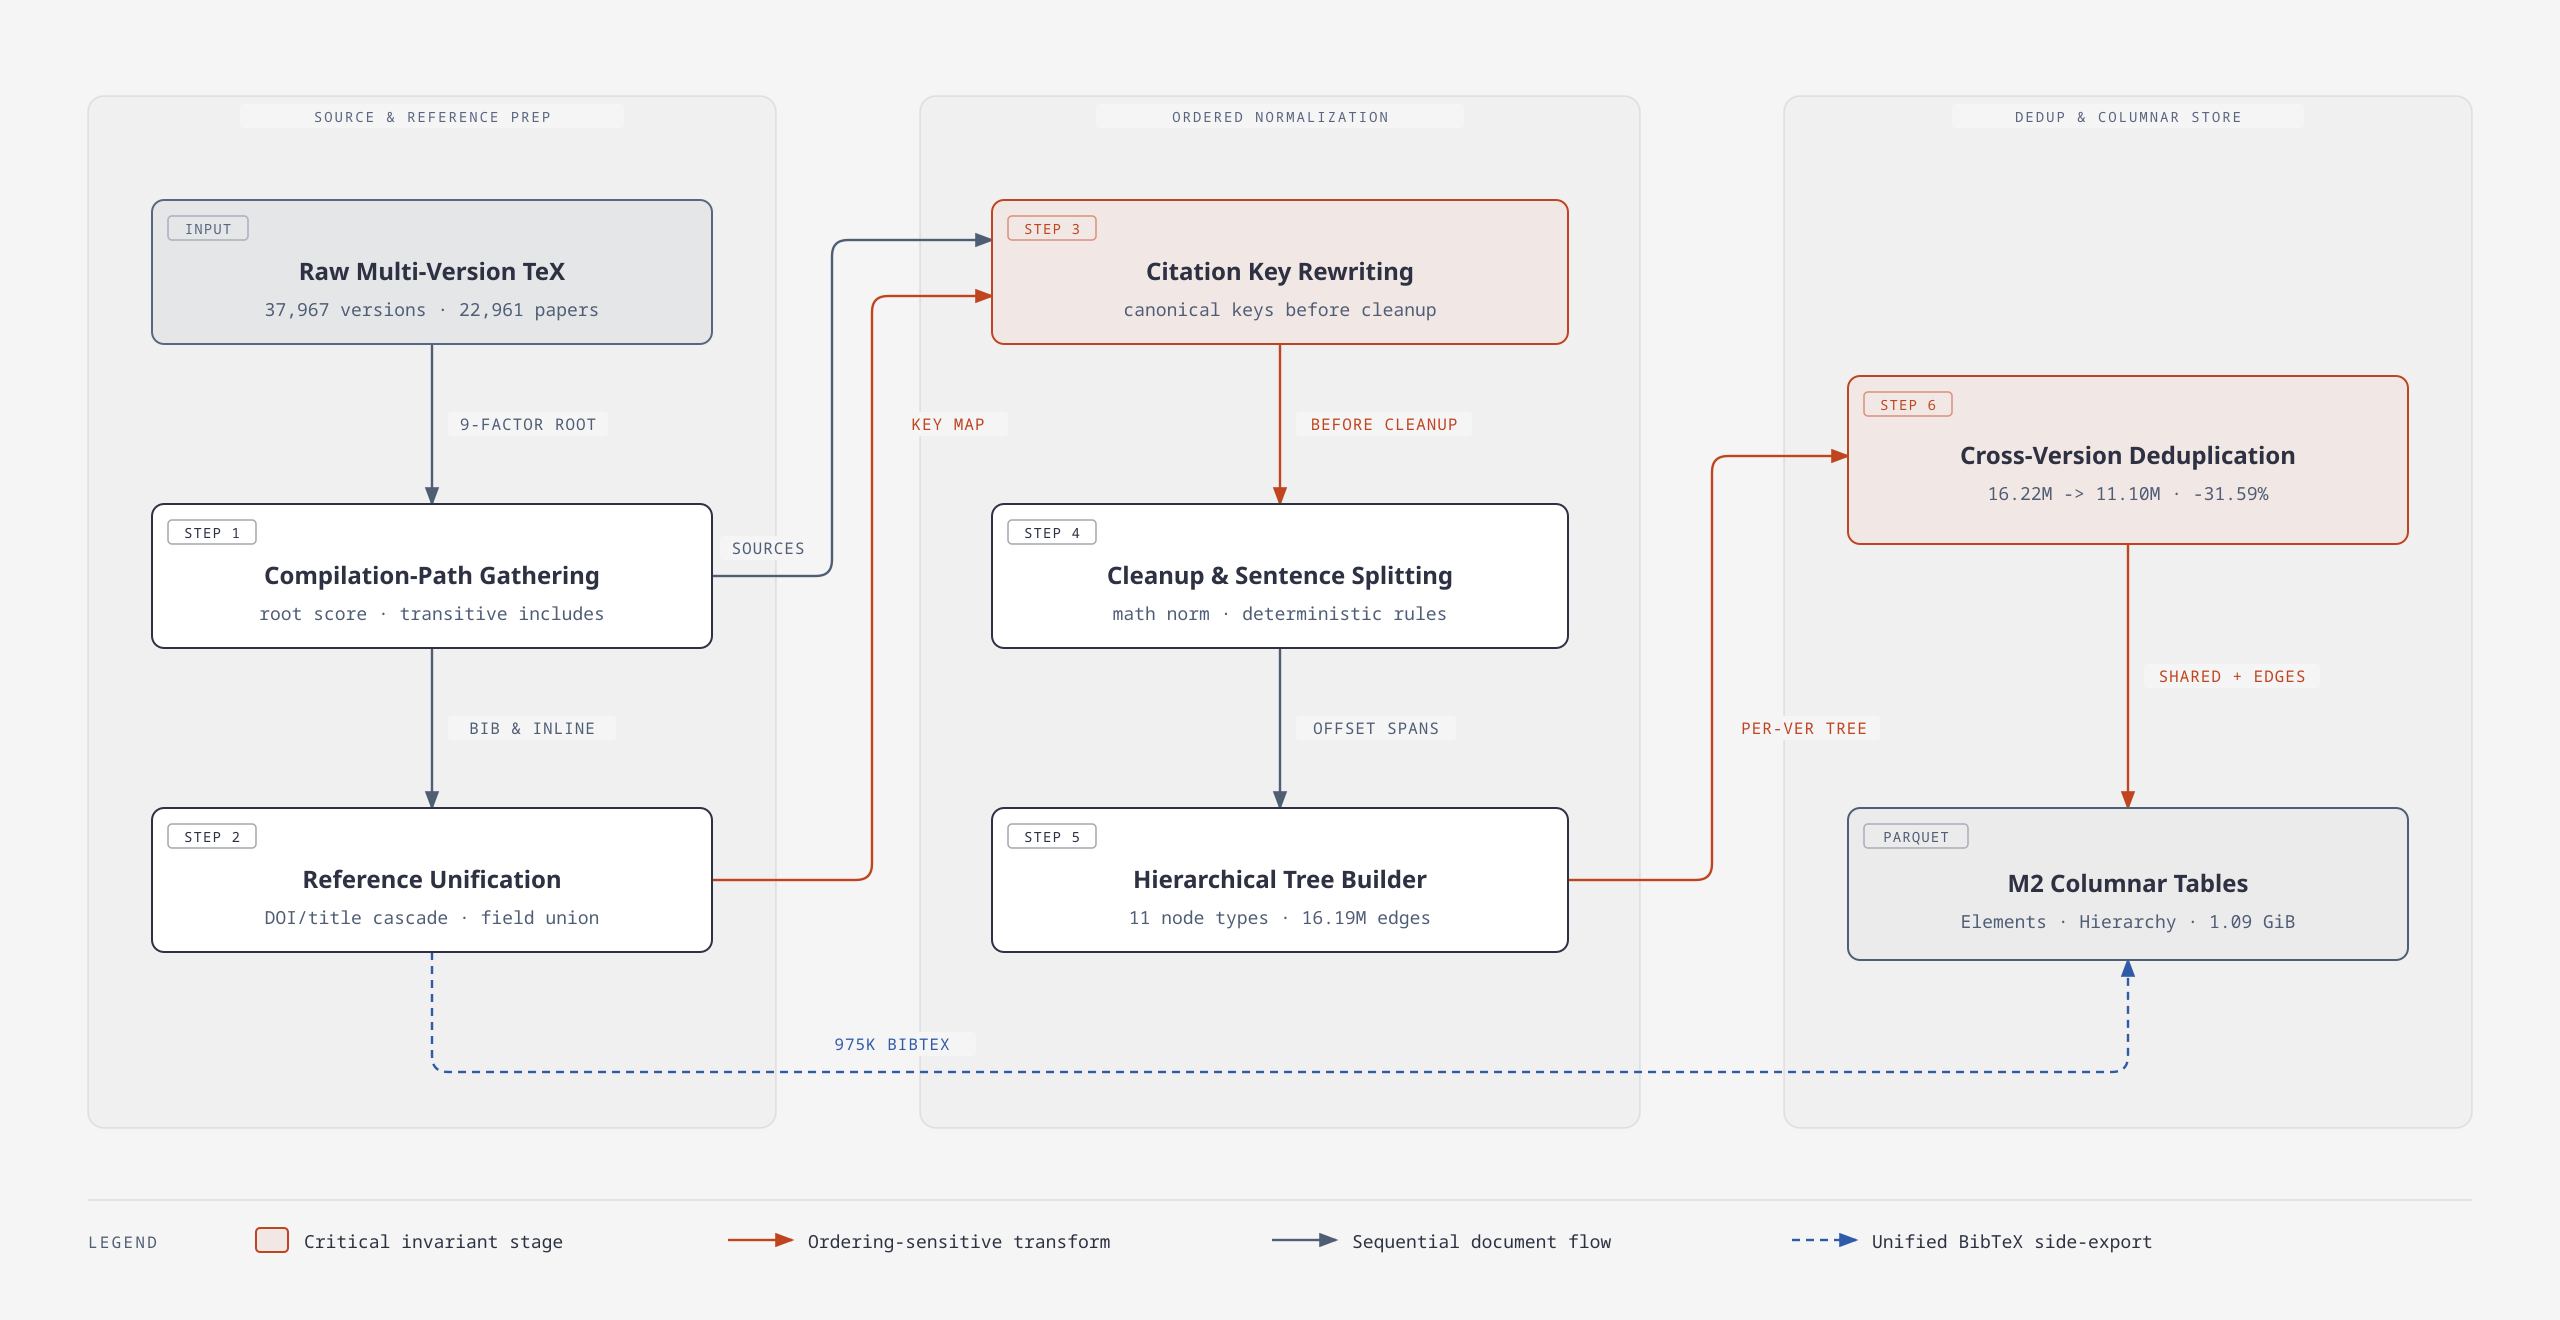
\includegraphics[width=\linewidth]{images/m2_parsing_dedup.png}
    \caption[Kiến trúc xử lý liên giai đoạn và khử trùng lặp của Giai đoạn 2]{Kiến trúc xử lý liên giai đoạn của Giai đoạn 2: gom tệp theo đường biên dịch, trích xuất và viết lại khóa trích dẫn trước khi dựng cây phân cấp, chuẩn hóa không chuỗi giữ chỗ và khử trùng lặp nội dung liên phiên bản.}
    \label{fig:m2_parsing_dedup}
\end{figure}

Một quyết định kiến trúc mang tính bản lề của Giai đoạn 2 nằm ở \textbf{thứ tự xử lý liên giai đoạn} giữa trích xuất thư mục tham khảo và dựng cây nội dung, được minh họa trong Hình~\ref{fig:m2_parsing_dedup}. Nếu dựng cây phân cấp, tách câu và băm khử trùng lặp trước rồi mới hợp nhất tài liệu tham khảo sau, hệ thống sẽ gặp lỗi lệch khóa trên các bài báo đa phiên bản. Cụ thể, khi tác giả đổi tên khóa trích dẫn của cùng một bài tham khảo giữa hai phiên bản nhưng giữ nguyên toàn bộ câu văn xuôi, hai câu hoàn toàn tương đương về ngữ nghĩa sẽ mang chuỗi khóa khác nhau và thất bại khi đối sánh khử trùng lặp toàn văn. Đồng thời, các lệnh trích dẫn còn lưu trong bảng phần tử nội dung sẽ không khớp với khóa chuẩn trong bảng mục lục BibTeX hợp nhất. Vì vậy, dây chuyền đảo ngược thứ tự xử lý: ngay sau bước gom tệp đa nguồn cho mọi phiên bản của một bài báo, thành phần trích xuất và hợp nhất thư mục tham khảo chạy trước tiên để ánh xạ mọi khóa cục bộ về khóa chuẩn và viết lại trực tiếp các lệnh trích dẫn trong luồng nguồn của từng phiên bản. Chỉ sau khi khóa chuẩn đã lan truyền đồng bộ vào toàn bộ văn bản, các bước dựng cây phân cấp, làm sạch LaTeX, chuẩn hóa toán học, tách câu và khử trùng lặp nội dung mới được thực thi.

\subsection{Dựng cây phân cấp tự động, chuẩn hóa và tách câu theo lát cắt bù trừ}

Trên luồng mã nguồn đã đồng bộ khóa trích dẫn của từng phiên bản, bộ dựng cây cấu trúc tự động loại bỏ chú thích dòng, các môi trường chú thích lồng nhau (trong khi giữ nguyên các khối mã nguyên văn) cùng các khai báo định nghĩa lệnh tùy biến trong phần thân để phần thân lệnh không sinh ra tiêu đề mục giả. Bộ quét luồng sau đó duyệt tuyến tính qua phần thân tài liệu và duy trì một ngăn xếp phạm vi phân cấp nhằm gán nút cha hiện hành cho từng thành phần mới. Ngăn xếp khởi đầu bằng nút gốc phiên bản tài liệu ở độ sâu $0$, tiếp nối bởi năm cấp tiêu đề giảm dần gồm chương, mục chính, tiểu mục cấp hai, tiểu mục cấp ba và tiêu đề đoạn văn (độ sâu từ $1$ đến $5$, trong đó cấp chương được quy về loại mục chính để giữ nhất quán lược đồ). Đối với danh sách có thứ tự và không thứ tự, khung danh sách nhận độ sâu bằng độ sâu nút cha cộng $10$ và mỗi mục con bên trong nhận độ sâu cộng thêm $1$, nhờ đó hỗ trợ danh sách lồng nhau nhiều tầng mà không xung đột cấp bậc với cấu trúc mục. Ở tầng thấp nhất, cây phân cấp chỉ chấp nhận nghiêm ngặt ba loại nút lá kết thúc không bao giờ đẩy vào ngăn xếp: câu văn xuôi, công thức toán học dạng khối và hình vẽ (hợp nhất cả hình ảnh, bảng dữ liệu, hình bảng bao văn bản và bảng nhiều trang về cùng loại nút lá hình vẽ theo đặc tả \cite{hcmus_intro_ds}).

Cơ chế tháo ngăn xếp tự động giúp bộ dựng cây thích ứng bền vững với cấu trúc soạn thảo phi chuẩn trong kho tiền ấn. Khi gặp một tiêu đề mới ở cấp $\ell$, ngăn xếp tự động bật bỏ mọi khung đang mở có độ sâu lớn hơn hoặc bằng $\ell$ nhưng luôn dừng lại trước nút gốc độ sâu $0$. Nhờ quy tắc này, các bài báo nhảy cấp trực tiếp từ mục chính xuống tiểu mục cấp ba hoặc bỏ quên lệnh đóng danh sách trước khi mở mục mới vẫn sinh cây hợp lệ. Tương tự, các lệnh đóng danh sách mồ côi sẽ bị bỏ qua an toàn nếu không tồn tại khung danh sách tương ứng trên ngăn xếp. Về phạm vi chọn lọc, mọi mục mang tiêu đề tham khảo đã chuẩn hóa cùng các môi trường hoặc chỉ thị danh mục tài liệu tham khảo đều bị loại trừ; ngược lại, mục lời cảm ơn không đánh số vẫn được giữ như mục bình thường, và chỉ thị phụ lục sau danh mục tham khảo lập tức đặt lại cờ loại trừ để bảo toàn trọn vẹn nội dung phụ lục. Sau khi quét xong, mọi cây phiên bản đều đi qua trình kiểm định tự động sáu bất biến cấu trúc: cho phép cây rỗng với phiên bản thiếu nguồn TeX, bắt buộc đúng một nút gốc không cha thuộc loại tài liệu với cây không rỗng, mọi liên kết cha phải trỏ tới nút tồn tại trong cùng phiên bản, mã định danh tạm phải duy nhất, loại nút phải thuộc tập từ vựng đóng và đồ thị cha--con tuyệt đối không chứa chu trình.

Song song với phân tích cấu trúc, nội dung văn bản và công thức đi qua bộ chuẩn hóa LaTeX bảo toàn một lượt quét. Thiết kế này xuất phát từ đánh đổi kỹ thuật cốt lõi: thực thi TeX đầy đủ quá tốn kém và kém an toàn với lệnh tự định nghĩa, còn việc xóa thô bằng biểu thức chính quy dễ phá hủy biểu thức toán và ký hiệu mảng trong ngoặc vuông. Do đó, bộ làm sạch bỏ qua nguyên vẹn mọi vùng toán học và giữ lại mọi lệnh chuyên ngành chưa rõ ngữ nghĩa, chỉ loại bỏ các chỉ thị trình bày phi ngữ nghĩa như căn chỉnh, ngắt trang, đường kẻ bảng ngang, khoảng trắng đứng ngang, cỡ chữ, gán thanh ghi độ dài hay bộ đếm đủ số đối số, gán thụt lề và khai báo định nghĩa lệnh. Các lệnh nhấn mạnh văn xuôi như in đậm, in nghiêng, gạch chân cùng các lớp bọc bố cục hai cột hoặc co giãn tỷ lệ được bóc vỏ đệ quy để bảo toàn nội dung thuần bên trong, áp dụng tương tự cho chú thích hình và bảng. Đặc biệt, thao tác xóa tùy chọn đặt vị trí hình nổi được thiết kế theo ngữ cảnh, chỉ kích hoạt ngay sau thẻ mở môi trường hình hoặc bảng nhằm bảo toàn tuyệt đối ký hiệu khoảng đóng và chỉ số mảng đặt trong ngoặc vuông giữa văn xuôi. Tiếp đó, bộ chuẩn hóa công thức toán kiểm tra tính chẵn lẻ dấu gạch chéo ngược để không nhận nhầm ký hiệu tiền tệ thoát hay lệnh xuống dòng, đưa mọi công thức nội tuyến về cặp dấu đô-la đơn và thống nhất toàn bộ công thức khối (cặp dấu đô-la kép, ngoặc vuông khối, cùng các môi trường phương trình, căn hàng và nhóm công thức có hoặc không đánh số) về khối phương trình chuẩn duy nhất.

Ở bước tách khối văn xuôi thành từng câu, kỹ thuật truyền thống thường thay thế công thức toán, lệnh LaTeX và địa chỉ mạng bằng các mã thẻ giữ chỗ nhân tạo trước khi đưa qua bộ tách câu, rồi đối sánh chuỗi để ghép ngược văn bản gốc. Thực tế triển khai trên văn bản khoa học bộc lộ điểm yếu nghiêm trọng của phương pháp này: khi bộ tách câu thống kê hoặc mạng nơ-ron tự chỉnh sửa khoảng trắng, tách dấu câu kề mã thẻ hoặc gặp cấu trúc ngoặc lồng nhau bên cạnh công thức, một số mã thẻ không thể khớp ngược và rò rỉ vĩnh viễn vào dữ liệu đầu ra. Hiện tượng này còn gây lệch ranh giới câu âm thầm, làm biến dạng nội dung toán học và phá vỡ phép so khớp khử trùng lặp giữa các phiên bản. Trên quy mô hơn $8.6$ triệu câu của kho dữ liệu, ngay cả tỷ lệ rò rỉ $0.1\%$ cũng đủ đưa hàng nghìn chuỗi lỗi vào bảng phần tử nội dung. Vì vậy, bài toán đòi hỏi một cơ chế bảo vệ cú pháp không can thiệp vào chuỗi gốc và loại bỏ hoàn toàn bước thay thế ngược.

Để giải quyết triệt để vấn đề trên, nhóm thiết kế kiến trúc \textbf{tách câu theo lát cắt bù trừ không dùng chuỗi giữ chỗ} dùng chung cho mọi bộ tách câu. Với đoạn văn xuôi đã làm sạch $T$ dài $n$ ký tự, bộ quét tuyến tính một lượt xác định tập khoảng bảo vệ rời nhau $\mathcal{P} = \{[a_k, b_k)\}_{k=1}^{m}$ bao phủ vùng toán học nội tuyến và khối, đối số ngoặc cân bằng của lệnh LaTeX, danh mục $20$ chữ viết tắt học thuật không phân biệt hoa thường (nhận diện cả khoảng trắng thường lẫn khoảng trống mỏng của TeX bên trong mà không nuốt khoảng trắng sau dấu chấm cuối), số thập phân cùng số hiệu phiên bản, địa chỉ thư điện tử và địa chỉ mạng có bảo toàn ngoặc cân bằng (chừa dấu chấm kết câu bên ngoài nhưng giữ ngoặc đóng cân bằng bên trong đường dẫn). Từ $\mathcal{P}$, hệ thống tạo hình chiếu che $M$ cùng độ dài tuyệt đối $|M| = |T| = n$:
\begin{equation}
    M[i] =
    \begin{cases}
        T[i] & \text{nếu } i \notin \bigcup_{k=1}^{m} [a_k, b_k) \text{ hoặc } T[i] \text{ là khoảng trắng}, \\
        \text{ký tự chữ cái trung tính} & \text{nếu } i \in \bigcup_{k=1}^{m} [a_k, b_k) \text{ và } T[i] \text{ không phải khoảng trắng}.
    \end{cases}
    \label{eq:m2_masked_view}
\end{equation}
Theo Phương trình~\eqref{eq:m2_masked_view}, hình chiếu $M$ bảo toàn chính xác từng tọa độ ký tự và mọi khoảng trắng của $T$, cho phép mọi bộ tách câu chỉ cần dự đoán tập vị trí kết thúc câu $\{e_j\}$ trên $M$. Các ranh giới ứng viên sau đó đi qua lớp hậu kiểm: gắn dấu ngoặc và ngoặc kép đóng liền kề về câu trước, hủy bỏ mọi vị trí cắt nằm bên trong khoảng thuộc $\mathcal{P}$ hoặc không đứng trước khoảng trắng hay cuối đoạn, và chỉ nhận ranh giới kết thúc bằng dấu chấm. Từng câu kết quả được trích xuất trực tiếp bằng lát cắt $T[s_j : e_j]$ trên chuỗi gốc nguyên vẹn $T$, triệt tiêu hoàn toàn nguy cơ rò rỉ chuỗi giữ chỗ hay sai lệch cú pháp LaTeX.

\subsection{Thực nghiệm so sánh các bộ tách câu trên CPU và quyết định lựa chọn}

Nhờ giao diện lát cắt bù trừ độc lập với thuật toán nhận diện ranh giới, nhóm tiến hành thực nghiệm so sánh có kiểm soát hai giai đoạn trên cùng máy CPU cục bộ (Intel Core i5-8365U 4 nhân 8 luồng, Python 3.12.13) đối với bốn bộ tách câu: bộ quy tắc kèm từ điển $20$ chữ viết tắt, bộ phát hiện không giám sát NLTK Punkt \cite{kiss2006}, mô hình nhận diện câu mạng nơ-ron cỡ nhỏ tiếng Anh của spaCy \cite{spacy}, và mô hình Segment Any Text ba tầng gọn nhẹ chạy trên bộ thực thi ONNX CPU \cite{frohmann2024}. Ở Giai đoạn 1, nhóm khảo sát $11$ bài báo TeX gồm $1{,}574$ khối văn xuôi, đánh giá đồng thời độ chính xác trên $12$ trường hợp biên khó tuyển chọn (như tên viết tắt tác giả, viết tắt học thuật hiếm ngoài từ điển và dấu câu kề ngoặc) cùng $40$ bài kiểm thử tương thích hợp đồng cú pháp. Kết quả ở phần trên của Bảng~\ref{tab:m2_tokenizer_study} chỉ ra sự đánh đổi rõ rệt giữa nhận diện ngữ cảnh và kỷ luật cấu trúc. Hai mô hình mạng nơ-ron nâng điểm chẩn đoán biên khó từ $7/12$ (bộ quy tắc) và $8/12$ (Punkt) lên $10/12$ (spaCy) và $9/12$ (Segment Any Text) nhờ khái quát tốt tên viết tắt ngoài từ điển. Ngược lại, tỷ lệ tuân thủ hợp đồng giảm từ $40/40$ ở bộ quy tắc xuống $38/40$ ở Punkt, $35/40$ ở spaCy và $27/40$ ở Segment Any Text do các mô hình học máy thỉnh thoảng gộp câu qua vùng chữ cái che kỹ thuật, trong khi Segment Any Text đã tiêu tốn $222.13\text{ s}$ chỉ trên $11$ bài báo.

\begin{table}[H]
    \centering
    \footnotesize
    \setlength{\tabcolsep}{4pt}
    \renewcommand{\arraystretch}{1.22}
    \begin{tabularx}{\textwidth}{@{}X c c r r@{}}
        \toprule
        \multicolumn{5}{@{}l@{}}{\textbf{(a) Nghiên cứu chẩn đoán và hồi quy trên 11 bài báo TeX (1,574 khối văn xuôi)}} \\
        \midrule
        \textbf{Bộ tách câu} & \textbf{Chẩn đoán (/12)} & \textbf{Hợp đồng (/40)} & \textbf{Số câu tách} & \textbf{Thời gian (s)} \\
        \midrule
        Quy tắc + từ điển 20 viết tắt & 7 / 12 & \textbf{40 / 40} & 5,635 & \textbf{0.54 -- 0.80} \\
        NLTK Punkt \cite{kiss2006} & 8 / 12 & 38 / 40 & 5,630 & 0.79 \\
        spaCy mạng nơ-ron \cite{spacy} & \textbf{10 / 12} & 35 / 40 & 5,608 & 3.37 \\
        Segment Any Text (ONNX CPU) \cite{frohmann2024} & 9 / 12 & 27 / 40 & 5,466 & 222.13 \\
        \bottomrule
    \end{tabularx}

    \vspace{0.8em}

    \begin{tabularx}{\textwidth}{@{}X r r r r r@{}}
        \toprule
        \multicolumn{6}{@{}l@{}}{\textbf{(b) Đo hiệu năng hệ thống trên dải 100 mã bài CPU (93 bài TeX, 7,525 khối, 4.80 triệu ký tự)}} \\
        \midrule
        \textbf{Cấu hình mô hình nơ-ron} & \textbf{Tổng (s)} & \textbf{s / pb} & \textbf{RAM (MiB)} & \textbf{Thông lượng} & \textbf{Ước tính 40k pb} \\
        \midrule
        spaCy (cỡ lô 1) \cite{spacy} & 17.28 & 0.186 & \textbf{151.5} & 278k ký tự/s & 2.06 giờ \\
        spaCy (cỡ lô 32) \cite{spacy} & \textbf{9.70} & \textbf{0.104} & 163.6 & \textbf{495k ký tự/s} & \textbf{1.16 giờ} \\
        Segment Any Text (cỡ lô 1) \cite{frohmann2024} & 1,283.91 & 13.805 & 1,310.1 & 3.74k ký tự/s & 153.39 giờ \\
        \bottomrule
    \end{tabularx}
    \caption[So sánh thực nghiệm bốn bộ tách câu trên môi trường CPU cục bộ]{Kết quả thực nghiệm so sánh bốn bộ tách câu trên cùng môi trường CPU cục bộ (Intel Core i5-8365U 4 nhân 8 luồng, Python 3.12.13). Ở thử nghiệm dải 100 mã bài, 6 bài chỉ có PDF và 1 bài vượt ngưỡng thời gian chờ; công đoạn chuẩn bị kho văn bản (giải nén, gom tệp, làm sạch và quét cấu trúc) tiêu tốn 35.89 s.}
    \label{tab:m2_tokenizer_study}
\end{table}

Nhằm đo đạc khả năng mở rộng thực tế ở quy mô hàng chục nghìn phiên bản, Giai đoạn 2 triển khai phép đo hệ thống trên một dải $100$ mã bài liên tiếp. Dải đo chứa $93$ bài có nguồn TeX hợp lệ (gồm $7{,}525$ khối văn xuôi với $4{,}803{,}251$ ký tự), $6$ bài chỉ có PDF và $1$ bài quá hạn thời gian chờ; riêng bước chuẩn bị văn bản đầu vào mất $35.89\text{ s}$. Theo phần dưới của Bảng~\ref{tab:m2_tokenizer_study}, spaCy chạy đơn lẻ ở cỡ lô $1$ hoàn thành trong $17.28\text{ s}$ ($0.186\text{ s}$ mỗi phiên bản, bộ nhớ đỉnh $151.5\text{ MiB}$, thông lượng $278\text{ nghìn ký tự/s}$), tương ứng $2.06\text{ giờ}$ ngoại suy cho $40{,}000$ phiên bản. Khi bật gom lô cỡ $32$, spaCy tăng thông lượng $1.78$ lần lên $495\text{ nghìn ký tự/s}$ và giảm thời gian còn $9.70\text{ s}$ ($0.104\text{ s}$ mỗi phiên bản, bộ nhớ đỉnh $163.6\text{ MiB}$, ngoại suy $1.16\text{ giờ}$ cho $40{,}000$ phiên bản). Trái lại, Segment Any Text trên CPU cần tới $1{,}283.91\text{ s}$ ($13.805\text{ s}$ mỗi phiên bản, thông lượng chỉ $3.74\text{ nghìn ký tự/s}$) và chiếm $1{,}310.1\text{ MiB}$ bộ nhớ đỉnh. Mức tiêu thụ này chậm hơn $74.3\times$ so với spaCy cỡ lô $1$, chậm hơn $132.4\times$ so với spaCy cỡ lô $32$ và ngốn bộ nhớ gấp $8.0\times$ đến $8.6\times$, đẩy ước lượng $40{,}000$ phiên bản lên $153.39\text{ giờ}$ và hoàn toàn bất khả thi trên Google Colab CPU.

Dựa trên số liệu thực nghiệm hai giai đoạn, nhóm lựa chọn \textbf{bộ tách câu theo quy tắc kèm từ điển $20$ chữ viết tắt} cho toàn bộ lượt chạy sản xuất $25{,}000$ bài báo trên Google Colab CPU, đồng thời giữ nguyên spaCy gom lô và Segment Any Text như các lựa chọn cấu hình cho nghiên cứu mở rộng. Dù spaCy cỡ lô $32$ đạt điểm chẩn đoán biên khó cao hơn ($10/12$) với chi phí ngoại suy chấp nhận được ($1.16\text{ giờ}$), bộ quy tắc vượt trội về độ tin cậy vận hành trên hạ tầng đám mây phân tán của năm thành viên. Trước hết, bộ quy tắc không yêu cầu tải trọng số mô hình ngoài nên loại bỏ hoàn toàn chi phí cài đặt môi trường và nguy cơ sai khác phiên bản mô hình khi phiên Colab khởi động lại. Thứ hai, bộ quy tắc đạt độ tuân thủ tuyệt đối $40/40$ với hợp đồng cấu trúc và bảo đảm tính tất định từng bit, giúp dấu vân tay kiểm chứng điểm phục hồi luôn khớp chính xác qua các lượt chạy nối tiếp. Cuối cùng, chi phí CPU và bộ nhớ không đáng kể của bộ quy tắc giữ ổn định dung lượng RAM cho tiến trình ghi điểm phục hồi quan hệ và xuất tệp cột Parquet trên máy ảo hai nhân xử lý.

\subsection{Trích xuất thư mục tham khảo và khử trùng lặp hai mức liên phiên bản}

Chiến lược khử trùng lặp trong Giai đoạn 2 gồm hai tầng nối tiếp: \textbf{Mức 1} trích xuất và hợp nhất thư mục tham khảo liên phiên bản trước khi phân tích văn bản, và \textbf{Mức 2} khử trùng lặp toàn văn các phần tử cấu trúc cùng nút lá sau khi chuẩn hóa. Ở Mức 1, bộ trích xuất xử lý đồng thời ba định dạng thư mục phổ biến trong kho arXiv. Với các tệp BibTeX bên ngoài được gọi từ văn bản hoạt động, bộ phân tích đếm cân bằng ngoặc nhọn và ngoặc tròn, hỗ trợ mở rộng định nghĩa chuỗi văn bản kèm phép nối chuỗi, bỏ qua khối tiền sảnh hay chú thích nhưng chỉ lược bỏ ký tự phần trăm chú thích \emph{giữa} các mục để không bao giờ cắt cụt ký tự mã hóa phần trăm bên trong địa chỉ URL. Với các mục tham khảo nội tuyến trong khối danh mục tài liệu tham khảo (gồm cả môi trường chuẩn lẫn chỉ thị gọi trực tiếp), hệ thống phối hợp dấu phân cách khối, trích xuất tiêu đề trong ngoặc kép LaTeX hoặc ngoặc cong, nhận diện tên tác giả có chữ cái đầu nối gạch ngang và định dạng họ đặt trước, bảo toàn tên nhóm hợp tác khoa học trong ngoặc vuông đi kèm dạng tác giả rút gọn và giải mã dấu phụ TeX về Unicode NFC. Đặc biệt, bộ trích xuất năm công bố bốn chữ số lọc bỏ vùng URL và DOI trước khi quét, đồng thời loại trừ mọi chuỗi bốn chữ số đứng liền trước dấu chấm thập phân để không nhận nhầm mã định danh arXiv hiện đại thành năm xuất bản. Ngoài ra, bộ trích xuất còn hỗ trợ các khối thư mục chuẩn AMSRefs với trường tác giả lặp lại trong ngoặc nhọn cùng trường ngày tháng và mã bản thảo điện tử, đồng thời chỉ thu nhận những mục có khóa thực sự xuất hiện trong lệnh trích dẫn hoạt động trừ khi bản thảo yêu cầu nạp toàn bộ thư mục.

Khi hợp nhất danh sách mục tham khảo từ mọi phiên bản của một bài báo được sắp xếp theo thứ tự thời gian tăng dần, hệ thống áp dụng tầng định danh ba bước nhằm nhận diện chính xác cùng một công trình dù khóa trích dẫn hay dấu câu thay đổi giữa các lần chỉnh sửa:
\begin{equation}
    \mathcal{I}(r) =
    \begin{cases}
        \text{DOI chuẩn hóa}(r) & \text{nếu } r \text{ có DOI hợp lệ}, \\
        \text{Tiêu đề ASCII chuẩn hóa}(r) & \text{nếu } |\tilde{t}(r)| \ge 8 \text{ và } |W(\tilde{t}(r))| \ge 2, \\
        \text{Khóa trích dẫn thường hóa}(r) & \text{chỉ khi thiếu cả hai định danh trên}.
    \end{cases}
    \label{eq:m2_bib_identity}
\end{equation}
Trong Phương trình~\eqref{eq:m2_bib_identity}, DOI chuẩn hóa (chữ thường, đã lược tiền tố đường dẫn phân giải và dấu câu thừa) là căn cứ đối sánh quyết định. Tầng thứ hai dùng tiêu đề đã phân rã Unicode NFKD, gập về ký tự ASCII chữ thường chỉ giữ chữ và số, nhưng buộc đạt tối thiểu $8$ ký tự và ít nhất $2$ từ nhằm tránh gộp nhầm các chuỗi ngắn chung chung. Tầng thứ ba chỉ kích hoạt khi thiếu cả DOI lẫn tiêu đề đáng tin cậy. Để ngăn gộp sai và hỏng đồ thị trích dẫn, thuật toán thi hành đồng bộ bốn rào chắn an toàn: một bản ghi thiếu DOI không được phép bắc cầu nối hai mục chuẩn mang hai DOI khác nhau; nếu cùng một khóa xuất hiện hai lần trong \emph{cùng một phiên bản} để chỉ hai công trình phân biệt, tầng đối sánh theo khóa bị tắt, khe khóa bị đánh dấu mơ hồ kèm nhật ký xung đột và bước viết lại trích dẫn sẽ chủ động bỏ qua khóa đó (cũng như chặn các phiên bản sau ánh xạ tới khóa từng mơ hồ ở phiên bản gốc); khóa chuẩn đầu ra luôn chọn theo phiên bản sớm nhất và tự gắn hậu tố số tất định khi hai công trình độc lập tình cờ dùng trùng khóa cục bộ; và phép gộp siêu dữ liệu thực hiện hợp không phá hủy bằng cách giữ nguyên trường đã có, điền bổ sung các trường còn thiếu và gom thêm mọi tên tác giả phân biệt mới xuất hiện. Bản đồ ánh xạ khóa sau hợp nhất lập tức được dùng để viết lại mọi lệnh trích dẫn trên luồng LaTeX của từng phiên bản trước bước dựng cây.

Sau khi toàn bộ các phiên bản của bài báo đã được viết lại khóa trích dẫn, dựng cây phân cấp, làm sạch LaTeX và chuẩn hóa toán học, cơ chế \textbf{khử trùng lặp toàn văn Mức 2} tiến hành hợp nhất nội dung trên phạm vi toàn bộ bài báo. Hệ thống duy trì một kho nội dung dùng chung cấp bài báo được lập chỉ mục theo cặp gồm loại phần tử và chuỗi văn bản đã chuẩn hóa khoảng trắng cùng dấu xuống dòng. Mỗi cặp khóa mới nhận một mã định danh chuẩn duy nhất gắn tiền tố bài báo và loại cấu trúc, đồng thời lưu đúng một dòng vào bảng phần tử nội dung; mọi lần xuất hiện trùng khớp ở các phiên bản sau tái sử dụng nguyên mã định danh chuẩn này. Tuy nhiên, bộ khử trùng lặp áp đặt hai ngoại lệ bảo toàn cấu trúc bắt buộc nhằm giữ đúng ngữ nghĩa cây phân cấp. Thứ nhất, nút gốc phiên bản tài liệu luôn giữ mã định danh riêng theo từng số phiên bản để mỗi phiên bản có điểm khởi đầu phân biệt trong đồ thị. Thứ hai, các vật chứa danh sách và mục danh sách mang nội dung khung mẫu rỗng ngữ nghĩa không bao giờ bị gộp giữa các lần xuất hiện, tránh tình trạng nhiều nhánh danh sách độc lập ở các mục khác nhau sập chung về một nút cha duy nhất.

Ở lượt duyệt thứ hai trên từng cây phiên bản, toàn bộ liên kết cha--con theo mã tạm cục bộ được ánh xạ sang cặp mã định danh chuẩn và lưu vào bảng quan hệ phân cấp kèm mã bài báo cùng số hiệu phiên bản, đồng thời loại bỏ mọi cạnh tự trỏ suy biến nếu có. Nhờ đó, bộ đếm lượt xuất hiện phần tử thô và bộ đếm phần tử duy nhất luôn đối khớp chính xác theo từng bài báo, giúp định lượng trực tiếp mức tiết kiệm dung lượng ở quy mô kho. Kiến trúc tách biệt bảng nội dung dùng chung và bảng cạnh theo phiên bản cho phép truy xuất chính xác cấu trúc nguyên vẹn của bất kỳ phiên bản nào chỉ bằng phép lọc theo số phiên bản mà không phải nhân bản văn bản. Bên cạnh đó, những phiên bản không chứa mã nguồn TeX hợp lệ được ghi nhận tường minh là phiên bản rỗng gồm không phần tử thay vì bị loại bỏ lặng lẽ khỏi đầu ra. Cơ chế ghi nhận tường minh này bảo đảm các báo cáo kiểm định luôn phân tách rõ ràng giữa độ phủ phiên bản trong kho lưu trữ và tỷ lệ phiên bản phân tích được nội dung LaTeX.

\subsection{Thống kê toàn bộ kho dữ liệu 25,000 bài báo và đánh giá dung lượng}

Kết quả vận hành Giai đoạn 2 trên toàn bộ $25{,}000$ bài báo của năm thành viên tạo nên kho dữ liệu phân cấp hoàn chỉnh với độ phủ đồng đều qua năm dải thời gian, được tổng hợp chi tiết trong Bảng~\ref{tab:m2_owner_stats}. Toàn kho đạt $22{,}961$ trên $25{,}000$ bài báo có tối thiểu một phần tử nội dung ($91.84\%$) và $2{,}039$ bài báo rỗng không có nguồn TeX ($8.16\%$). Ở cấp độ phiên bản, $37{,}967$ trên $40{,}896$ phiên bản khai báo được dựng cây thành công, tương ứng tỷ lệ phủ $92.84\%$. So với mức độ sẵn có nguồn TeX khoảng $97\%$ được ghi nhận trên arXiv \cite{ginev2024}, độ chênh khoảng $4$--$5$ điểm phần trăm bắt nguồn từ các bài chỉ nộp PDF, gói lưu trữ không hỗ trợ đã sàng lọc ở Giai đoạn 1 và tỷ lệ nhỏ gói nguồn thiếu thân tài liệu hợp lệ. Sự ổn định xuyên suốt năm dải dữ liệu được thể hiện rõ khi tỷ lệ bài phân tích thành công nằm gọn từ $90.88\%$ đến $93.28\%$ và tỷ lệ phiên bản đạt từ $92.01\%$ đến $94.08\%$. Đáng chú ý, dữ liệu xuất bản thỏa mãn tuyệt đối đẳng thức kiểm định toàn vẹn cây: $16{,}185{,}255$ cạnh phân cấp cộng với đúng $37{,}967$ nút gốc phiên bản bằng chính xác $16{,}223{,}222$ lượt xuất hiện phần tử thô trước khử trùng lặp, xác nhận không có bất kỳ nút lạc hay mất liên kết nào trên toàn hệ thống.

\begin{table}[H]
    \centering
    \footnotesize
    \setlength{\tabcolsep}{4pt}
    \renewcommand{\arraystretch}{1.18}
    \begin{tabularx}{\textwidth}{@{}X r r r r r r r@{}}
        \toprule
        \textbf{Thành viên} &
        \shortstack[r]{\textbf{Bài có TeX} \\ \textbf{(Tỷ lệ)}} &
        \shortstack[r]{\textbf{Phiên bản} \\ \textbf{(Tỷ lệ)}} &
        \shortstack[r]{\textbf{Lượt} \\ \textbf{thô}} &
        \shortstack[r]{\textbf{Duy nhất} \\ \textbf{(Giảm)}} &
        \shortstack[r]{\textbf{Cạnh} \\ \textbf{cây}} &
        \shortstack[r]{\textbf{BibTeX} \\ \textbf{(Số bài)}} &
        \shortstack[r]{\textbf{Parquet} \\ \textbf{(MiB)}} \\
        \midrule
        Trịnh Huỳnh Nhi &
            \shortstack[r]{4,578 \\ {\scriptsize (91.56\%)}} &
            \shortstack[r]{7,687 \\ {\scriptsize (92.97\%)}} &
            3,194,213 &
            \shortstack[r]{2,167,101 \\ {\scriptsize (-32.16\%)}} &
            3,186,526 &
            \shortstack[r]{195,076 \\ {\scriptsize (3,888)}} &
            217.22 \\
        \addlinespace[3pt]
        Ngô Mẫn Nhi &
            \shortstack[r]{4,544 \\ {\scriptsize (90.88\%)}} &
            \shortstack[r]{7,592 \\ {\scriptsize (92.01\%)}} &
            3,276,789 &
            \shortstack[r]{2,221,136 \\ {\scriptsize (-32.22\%)}} &
            3,269,197 &
            \shortstack[r]{195,360 \\ {\scriptsize (3,819)}} &
            222.02 \\
        \addlinespace[3pt]
        Huỳnh Huy Hoàng &
            \shortstack[r]{4,664 \\ {\scriptsize (93.28\%)}} &
            \shortstack[r]{7,888 \\ {\scriptsize (94.08\%)}} &
            3,262,182 &
            \shortstack[r]{2,198,596 \\ {\scriptsize (-32.60\%)}} &
            3,254,294 &
            \shortstack[r]{203,414 \\ {\scriptsize (3,923)}} &
            227.36 \\
        \addlinespace[3pt]
        Phạm Minh Trọng &
            \shortstack[r]{4,585 \\ {\scriptsize (91.70\%)}} &
            \shortstack[r]{7,449 \\ {\scriptsize (92.42\%)}} &
            3,334,790 &
            \shortstack[r]{2,288,312 \\ {\scriptsize (-31.38\%)}} &
            3,327,341 &
            \shortstack[r]{194,577 \\ {\scriptsize (3,868)}} &
            227.95 \\
        \addlinespace[3pt]
        Nguyễn Phúc Khang &
            \shortstack[r]{4,590 \\ {\scriptsize (91.80\%)}} &
            \shortstack[r]{7,351 \\ {\scriptsize (92.66\%)}} &
            3,155,248 &
            \shortstack[r]{2,223,044 \\ {\scriptsize (-29.54\%)}} &
            3,147,897 &
            \shortstack[r]{187,247 \\ {\scriptsize (3,706)}} &
            222.72 \\
        \midrule
        \textbf{Tổng toàn nhóm} &
            \shortstack[r]{\textbf{22,961} \\ {\scriptsize \textbf{(91.84\%)}}} &
            \shortstack[r]{\textbf{37,967} \\ {\scriptsize \textbf{(92.84\%)}}} &
            \textbf{16,223,222} &
            \shortstack[r]{\textbf{11,098,189} \\ {\scriptsize \textbf{(-31.59\%)}}} &
            \textbf{16,185,255} &
            \shortstack[r]{\textbf{975,674} \\ {\scriptsize \textbf{(19,204)}}} &
            \textbf{1,117.27} \\
        \bottomrule
    \end{tabularx}
    \caption{Thống kê kết quả phân tích cú pháp, khử trùng lặp, trích xuất thư mục tham khảo và dung lượng lưu trữ Parquet của Giai đoạn 2 trên toàn bộ 25,000 bài báo (40,896 phiên bản khai báo) theo năm thành viên.}
    \label{tab:m2_owner_stats}
\end{table}

Phân bố chi tiết của $11{,}098{,}189$ phần tử duy nhất theo $11$ loại cấu trúc được trình bày trong Bảng~\ref{tab:m2_kind_dist}. Ba loại nút lá nội dung chiếm tỷ trọng áp đảo $89.30\%$ ($9{,}910{,}699$ phần tử), bao gồm $8{,}634{,}050$ câu văn xuôi ($77.80\%$), $991{,}526$ công thức toán khối ($8.93\%$) và $285{,}123$ hình vẽ cùng bảng biểu ($2.57\%$). Tám loại nút cấu trúc chiếm $10.70\%$ còn lại ($1{,}187{,}490$ phần tử), tập trung nhiều nhất ở mục con danh sách ($4.45\%$), tiểu mục cấp hai ($2.00\%$) và mục chính cùng chương ($1.66\%$). Song song với kho nội dung phân cấp, bảng mục lục BibTeX hợp nhất chứa $975{,}674$ mục tham khảo duy nhất trích xuất từ $19{,}204$ bài báo ($76.82\%$ toàn kho), đạt trung bình $39.03$ mục mỗi bài trên toàn bộ $25{,}000$ bài và $50.81$ mục trên nhóm bài có thư mục. Phân loại tài liệu tham khảo phản ánh đặc trưng kho arXiv với $57.93\%$ bài báo tạp chí, $19.17\%$ tài liệu tổng hợp và tiền ấn, $18.25\%$ bài báo kỷ yếu hội nghị, $3.02\%$ sách chuyên khảo và $1.63\%$ loại khác. Tỷ lệ đầy đủ trường siêu dữ liệu đạt rất cao ở tiêu đề ($99.23\%$), năm công bố ($98.36\%$) và tác giả ($97.03\%$), tiếp theo là tạp chí hoặc nơi xuất bản ($71.11\%$), mã DOI ($34.13\%$) và đường dẫn URL ($20.64\%$). Độ phủ chênh lệch giữa ba trường cốt lõi và các mã định danh tường minh định hướng trực tiếp chiến lược trích chọn đặc trưng đa nhóm cho bài toán đối sánh trích dẫn ở Giai đoạn 3.

\begin{table}[H]
    \centering
    \footnotesize
    \renewcommand{\arraystretch}{1.22}
    \begin{tabularx}{\textwidth}{l X r r}
        \toprule
        \textbf{Nhóm vai trò} & \textbf{Loại phần tử cấu trúc} & \textbf{Số lượng duy nhất} & \textbf{Tỷ trọng (\%)} \\
        \midrule
        \multirow{3}{*}{Nút lá nội dung (89.30\%)}
            & Câu văn xuôi & 8,634,050 & 77.80\% \\
            & Công thức toán học dạng khối & 991,526 & 8.93\% \\
            & Hình vẽ và bảng biểu & 285,123 & 2.57\% \\
        \midrule
        \multirow{8}{*}{Nút cấu trúc vật chứa (10.70\%)}
            & Mục con trong danh sách & 493,812 & 4.45\% \\
            & Tiểu mục cấp hai & 222,075 & 2.00\% \\
            & Mục chính và chương & 184,592 & 1.66\% \\
            & Danh sách không thứ tự & 80,860 & 0.73\% \\
            & Tiểu mục cấp ba & 62,123 & 0.56\% \\
            & Danh sách có thứ tự & 57,865 & 0.52\% \\
            & Tiêu đề đoạn văn & 48,196 & 0.43\% \\
            & Nút gốc phiên bản tài liệu & 37,967 & 0.34\% \\
        \midrule
        \textbf{Tổng cộng} & \textbf{Toàn bộ phần tử duy nhất sau khử trùng lặp} & \textbf{11,098,189} & \textbf{100.00\%} \\
        \bottomrule
    \end{tabularx}
    \caption{Phân bố thành phần của 11,098,189 phần tử duy nhất theo nhóm nút lá và nút cấu trúc trên toàn bộ kho 25,000 bài báo.}
    \label{tab:m2_kind_dist}
\end{table}

Nhìn tổng thể hai giai đoạn đầu qua Hình~\ref{fig:m1_m2_stats}, hiệu quả kỹ thuật dữ liệu tích lũy qua hai tầng tinh gọn mang lại mức tiết kiệm dung lượng vượt bậc. Ở tầng thứ nhất, cơ chế trích xuất chọn lọc của Giai đoạn 1 trên $35{,}212$ phiên bản được đo đạc loại bỏ hình ảnh nhị phân cùng tệp biên dịch trung gian, thu gọn dung lượng trung bình gia quyền mỗi phiên bản từ $4.70\text{ MiB}$ ($4{,}926{,}068\text{ byte}$) xuống còn $296.7\text{ KiB}$ ($303{,}797\text{ byte}$), tương ứng mức giảm $93.83\%$. Ở tầng thứ hai, khử trùng lặp liên phiên bản của Giai đoạn 2 loại bỏ thêm $5{,}125{,}033$ lượt xuất hiện phần tử dư thừa trên tổng số $16{,}223{,}222$ lượt thô, đạt mức giảm $31.59\%$ nhờ tái sử dụng nội dung bất biến giữa các phiên bản trên $10{,}659$ bài báo đa phiên bản ($42.64\%$ toàn kho). Mối tương quan thực nghiệm giữa mật độ phiên bản và tỷ lệ giảm trùng thể hiện nhất quán trên từng dải thành viên: dải của Huỳnh Huy Hoàng có số phiên bản trung bình cao nhất ($1.677$ phiên bản/bài) nên đạt tỷ lệ giảm lớn nhất ($-32.60\%$), còn dải của Nguyễn Phúc Khang có mật độ phiên bản thấp nhất ($1.587$ phiên bản/bài) nên giảm ít nhất ($-29.54\%$). Nhờ kết hợp khử trùng lặp hai mức với lưu trữ hướng cột Apache Parquet \cite{apache_parquet}, toàn bộ ba bảng dữ liệu của $25{,}000$ bài báo chỉ chiếm $1{,}117.27\text{ MiB}$ ($1.091\text{ GiB}$) trên đĩa, gồm $902.35\text{ MiB}$ cho bảng phần tử nội dung, $126.41\text{ MiB}$ cho bảng mục lục BibTeX hợp nhất và $88.50\text{ MiB}$ cho toàn bộ $16.19$ triệu cạnh phân cấp.

\begin{figure}[H]
    \centering
    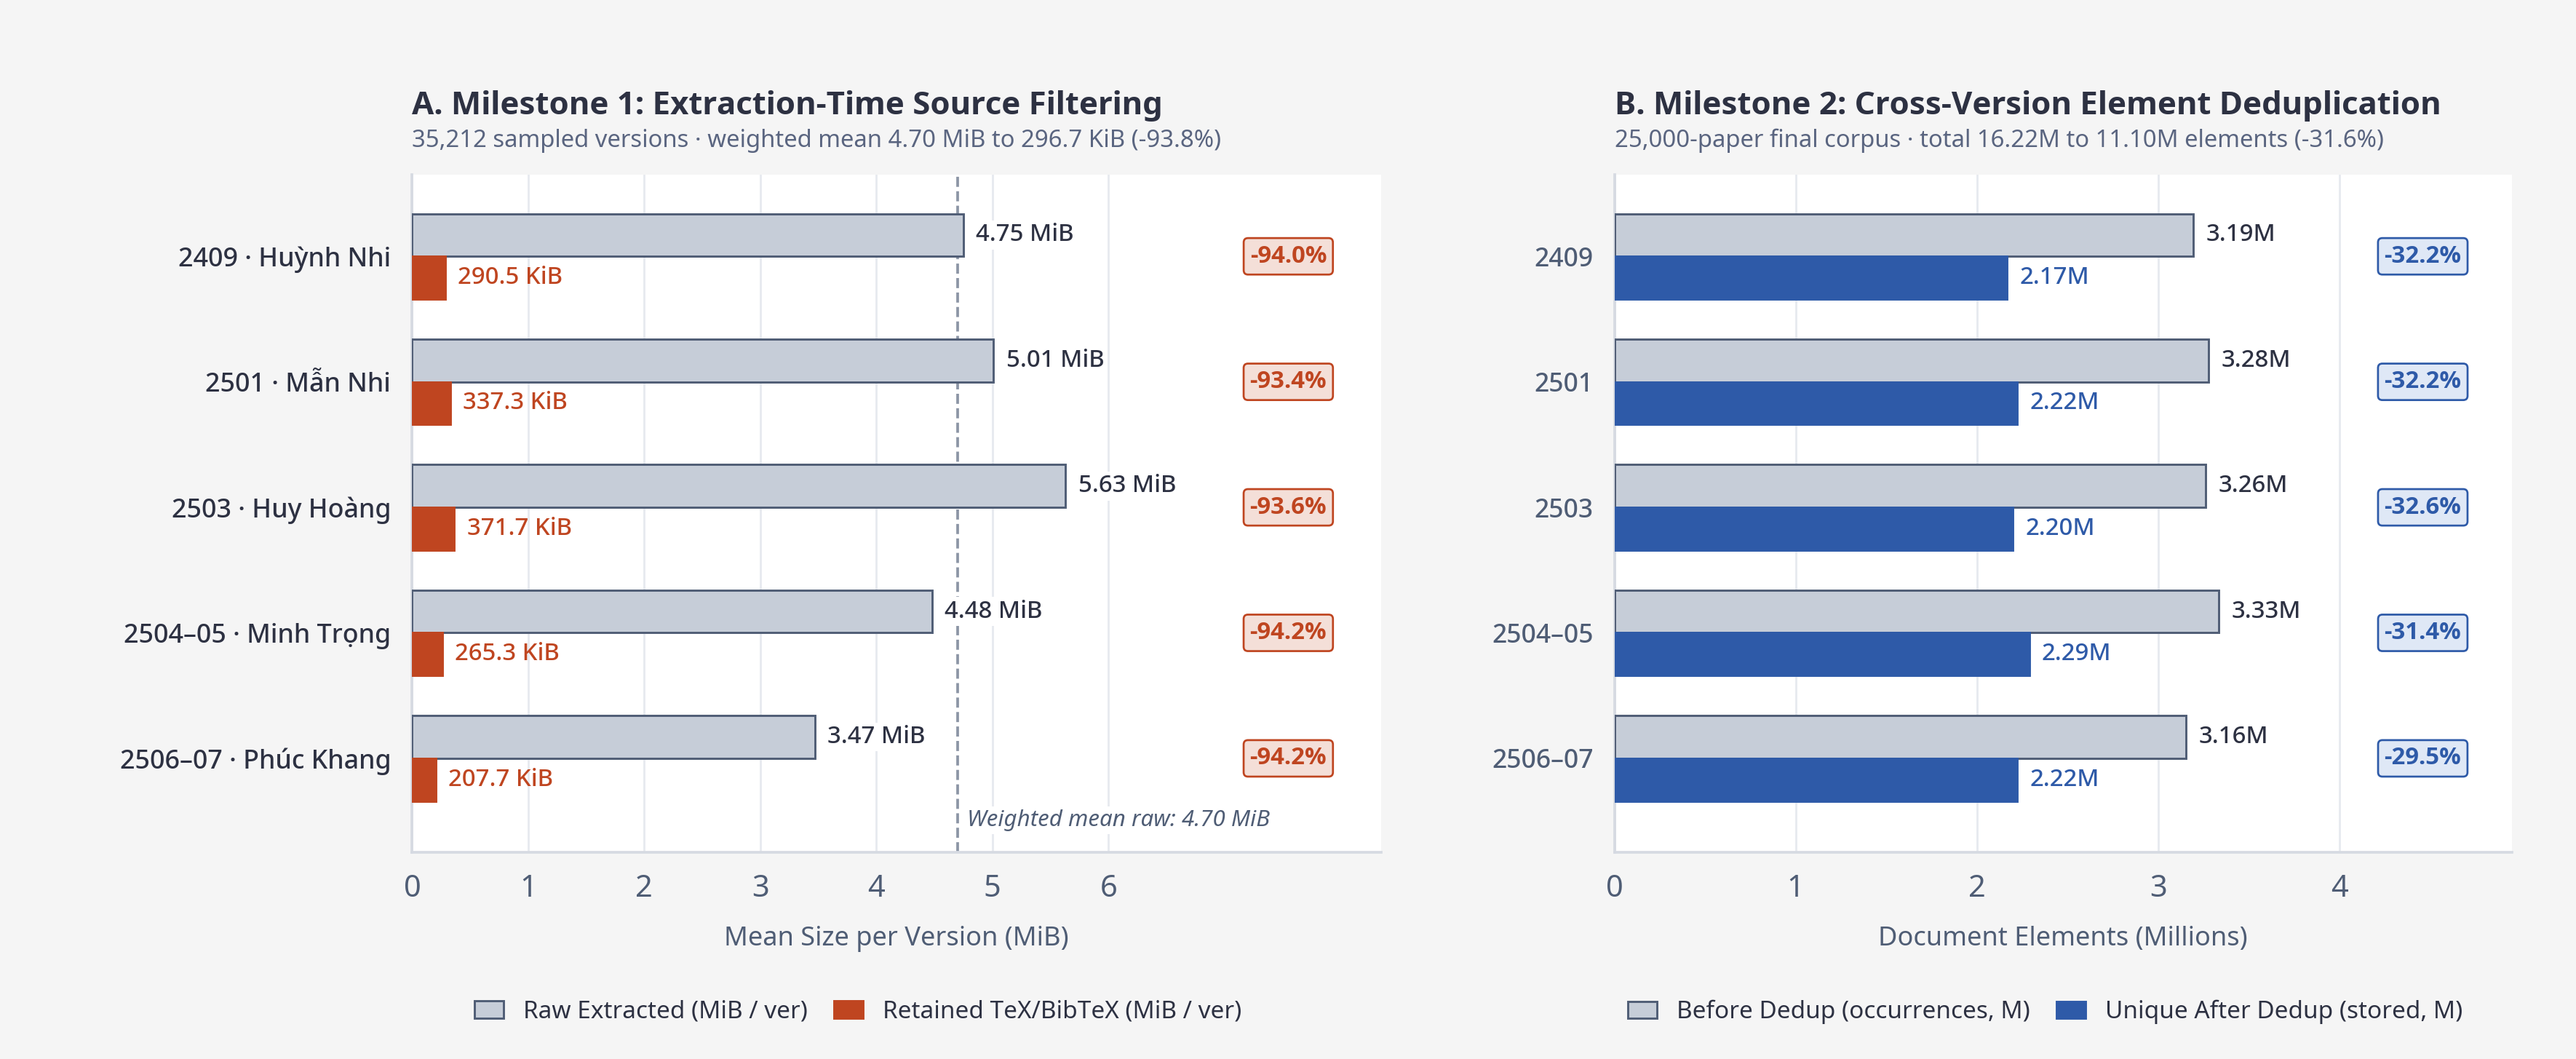
\includegraphics[width=\linewidth]{images/m1_m2_stats.png}
    \caption[Hiệu quả nén dữ liệu tích lũy ở Giai đoạn 1 và khử trùng lặp ở Giai đoạn 2]{Hiệu quả kỹ thuật dữ liệu tích lũy qua hai giai đoạn trên năm dải dữ liệu: mức nén dung lượng nguồn chọn lọc ở Giai đoạn 1 ($-93.83\%$ trên $35{,}212$ phiên bản mẫu) và tỷ lệ khử trùng lặp phần tử nội dung liên phiên bản ở Giai đoạn 2 ($-31.59\%$, từ $16.22$ triệu xuống $11.10$ triệu phần tử duy nhất).}
    \label{fig:m1_m2_stats}
\end{figure}

Về minh bạch số liệu thực nghiệm, cần ghi nhận rõ rằng nhật ký thời gian thực thi tổng thể và bộ nhớ đỉnh trên Google Colab CPU của lượt chạy sản xuất $25{,}000$ bài báo Giai đoạn 2 hiện được lưu trên kho sao lưu đám mây bên ngoài bản chụp cục bộ của dự án. Do không đưa các con số thiếu bản ghi kiểm chứng cục bộ vào báo cáo, toàn bộ phân tích định lượng về tốc độ xử lý, bộ nhớ tiến trình và khả năng mở rộng CPU của Giai đoạn 2 đều căn cứ chặt chẽ vào hai phép đo cục bộ tái lập hoàn toàn trong Bảng~\ref{tab:m2_tokenizer_study}. Trên hạ tầng Colab vốn dễ bị thu hồi máy ảo đột ngột, quy trình vận hành sản xuất bảo vệ tiến độ bằng cơ chế lưu điểm phục hồi quan hệ cục bộ sau từng bài báo. Song song đó, hệ thống định kỳ đồng bộ các thế hệ sao chụp bất biến ra kho lưu trữ ngoài kèm kiểm tra mã băm SHA-256 và đối chiếu dấu vân tay mã nguồn lẫn dữ liệu đầu vào trước khi đóng gói. Ba bảng Parquet đạt chuẩn kiểm định toàn vẹn cuối cùng trở thành nền dữ liệu sạch, thống nhất khóa trích dẫn và sẵn sàng cho bài toán học máy đối sánh tài liệu tham khảo ở Giai đoạn 3.

\section{Giai đoạn 3: Hệ thống đối sánh tài liệu tham khảo bằng học máy}

\subsection{Phát biểu bài toán xếp hạng ứng viên và thiết kế dữ liệu nhãn}

Trong cấu trúc kho dữ liệu học thuật sau hai giai đoạn đầu, mỗi bài báo trích dẫn $p$ sở hữu đồng thời một tập gồm $m_p$ mục thư mục BibTeX chuẩn hóa $\mathcal{E}_p = \{e_1, \dots, e_{m_p}\}$ trích xuất từ mã nguồn LaTeX và một tập gồm $n_p$ tài liệu tham khảo có định danh arXiv $\mathcal{R}_p = \{r_1, \dots, r_{n_p}\}$ thu hoạch từ đồ thị tri thức học thuật. Bài toán đối sánh tài liệu tham khảo được phát biểu dưới dạng phân giải thực thể nội bài báo trên không gian ứng viên tích Đề-các $\mathcal{E}_p \times \mathcal{R}_p$. Với mỗi mục truy vấn $e_i \in \mathcal{E}_p$, mô hình cần ước lượng hàm chấm điểm $f(e_i, r_j)$ cho từng ứng viên $r_j \in \mathcal{R}_p$ sao cho tài liệu tham khảo đúng $r^*_i$ (khi tồn tại trong $\mathcal{R}_p$) đạt thứ hạng cao nhất trong danh sách sắp xếp giảm dần, ưu tiên vị trí dẫn đầu trong nhóm năm ứng viên hàng đầu. Việc thu hẹp không gian ứng viên về phạm vi nội bài báo giúp giảm số ứng viên trung bình xuống còn vài chục tài liệu thay vì hàng trăm nghìn bản ghi toàn kho. Tuy nhiên, phạm vi nội bài báo lại tạo ra bài toán phân biệt tinh vi giữa các công trình cùng chủ đề, cùng nhóm tác giả hoặc các chuỗi bài báo nhiều phần thường được trích dẫn cạnh nhau trong một văn bản khoa học. Nhằm tuân thủ tuyến đánh giá chuẩn độc lập không dùng mô hình ngôn ngữ lớn hay vector nhúng huấn luyện sẵn theo quy định học phần~\cite{hcmus_intro_ds}, hệ thống đối chiếu trực tiếp hai họ học máy có cơ chế tối ưu bổ trợ nhau: phân loại nhị phân điểm-theo-điểm bằng Hồi quy Logistic cân bằng trọng số lớp~\cite{pedregosa2011} và học xếp hạng theo danh sách bằng LightGBM LambdaRank tối ưu chỉ số NDCG@5~\cite{ke2017,burges2010}.

Để xây dựng tập dữ liệu giám sát đáng tin cậy trên toàn bộ kho $N = 25{,}000$ bài báo của năm thành viên, nhóm thiết kế quy trình gán nhãn hai tầng tách biệt hoàn toàn giữa tập chuẩn thủ công và tập tự động quy mô lớn. Ở tầng thủ công, mỗi thành viên chọn độc lập $5$ bài báo từ dải dữ liệu cá nhân để lập tập chuẩn gồm $25$ bài báo với $2{,}519$ mục BibTeX và $1{,}880$ cặp đối sánh đúng đã xác minh (phân bố gồm Ngô Mẫn Nhi $882$, Trịnh Huỳnh Nhi $510$, Phạm Minh Trọng $189$, Huỳnh Huy Hoàng $157$ và Nguyễn Phúc Khang $142$ cặp khớp). Mỗi bài báo thủ công đều đạt ít nhất $26$ cặp khớp, vượt định mức tối thiểu $20$ cặp mỗi bài, còn tổng số $1{,}880$ cặp của cả nhóm vượt xa ngưỡng $500$ cặp của đề bài. Toàn bộ tập thủ công được đối chiếu hoàn toàn từ đầu mà không điền sẵn gợi ý từ bộ quy tắc tự động nhằm triệt tiêu thiên lệch xác nhận và đảm bảo tính khách quan khi kiểm định ngược. Ở tầng tự động, hệ thống lấy mẫu $500$ bài báo mỗi thành viên từ phần kho còn lại, tạo thành $2{,}500$ bài báo ($10.01\%$ trong số $24{,}975$ bài báo ngoài tập thủ công) với $98{,}922$ mục BibTeX và $33{,}493$ cặp khớp. Gộp cả hai tầng, tập dữ liệu đối sánh toàn nhóm bao gồm $2{,}525$ bài báo ($1{,}934$ bài có ít nhất một mục BibTeX và $591$ bài không có mục BibTeX) với $101{,}441$ mục được phân loại trạng thái, gồm $35{,}373$ mục có đích khớp, $65{,}816$ mục không có đích khớp trong kho tham khảo arXiv, $242$ mục chưa rà soát và $10$ mục mơ hồ.

Bộ gán nhãn tự động cho $2{,}500$ bài báo được đóng băng trước giai đoạn huấn luyện dưới dạng bộ quy tắc tất định ba tầng nhằm cân bằng giữa độ chính xác cao và độ phủ rộng. Ở tầng thứ nhất, hệ thống trích xuất mã định danh arXiv xuất hiện tường minh trong mục BibTeX rồi đối chiếu trực tiếp với tập ứng viên của bài báo. Khi một mục chứa mã arXiv tường minh nhưng mã này hoàn toàn vắng mặt trong tập tài liệu tham khảo đã thu hoạch, quy tắc áp đặt cơ chế phủ quyết cứng kết luận không khớp nhằm ngăn các tầng mờ phía sau ghép nhầm vào một bài báo khác có tiêu đề gần giống. Ở tầng thứ hai, hệ thống đối chiếu trùng khớp chính xác trên tiêu đề đã chuẩn hóa, kết hợp kiểm tra tính nhất quán chữ số cho chuỗi công trình nhiều phần và phân tách bằng họ tác giả khi có nhiều ứng viên trùng tiêu đề. Ở tầng thứ ba, các mục chưa được quyết định ở hai tầng đầu phải đạt điểm chồng lấp và bao hàm từ vựng tiêu đề tối thiểu $0.65$, sau đó được hiệu chỉnh cộng $0.08$ khi trùng họ tác giả, cộng $0.04$ khi năm công bố gần nhau và trừ $0.15$ khi năm công bố cách xa. Một cặp ứng viên ở tầng thứ ba chỉ được chấp nhận khi điểm tổng hợp đạt ít nhất $0.82$, vượt cổng biên độ mơ hồ tối thiểu $0.10$ so với ứng viên xếp thứ hai và không vi phạm điều kiện phủ quyết biến thể từ ghép.

\begin{table}[htbp]
    \centering
    \scriptsize
    \renewcommand{\arraystretch}{1.20}
    \begin{tabularx}{\textwidth}{l r r r r X}
        \toprule
        \textbf{Phân vùng} & \textbf{Tổng bài} & \textbf{Thủ công} & \textbf{Tự động} & \textbf{Truy vấn} & \textbf{Cấu trúc truy vấn có đích khớp} \\
        \midrule
        Huấn luyện (Train) & $2{,}505$ & $15$ & $2{,}490$ & $34{,}334$ & $1{,}014$ thủ công + $33{,}320$ tự động \\
        Kiểm định (Valid)  & $10$      & $5$  & $5$       & $511$      & $435$ thủ công + $76$ tự động \\
        Kiểm tra (Test)    & $10$      & $5$  & $5$       & $528$      & $431$ thủ công + $97$ tự động \\
        \midrule
        \textbf{Tổng toàn nhóm} & $\mathbf{2{,}525}$ & $\mathbf{25}$ & $\mathbf{2{,}500}$ & $\mathbf{35{,}373}$ & $\mathbf{1{,}880}$ \textbf{thủ công +} $\mathbf{33{,}493}$ \textbf{tự động} \\
        \bottomrule
    \end{tabularx}
    \caption{Phân chia tập dữ liệu đối sánh ở cấp độ bài báo theo phân tầng năm thành viên (hạt giống ngẫu nhiên $42$)}
    \label{tab:m3_split}
\end{table}

Cuộc kiểm toán độc lập bộ quy tắc tự động ba tầng trên toàn bộ $25$ bài báo thủ công cho thấy chất lượng nhãn giám sát yếu đạt độ tin cậy cao với độ chính xác $98.72\%$ và độ phủ $98.83\%$, tương ứng $1{,}858$ cặp khớp đúng, $373$ trường hợp không khớp đúng, $24$ trường hợp ghép sai và $22$ trường hợp bỏ sót. Phân rã sâu theo từng tầng quy tắc chỉ rõ bản chất sai số của bộ quy tắc: cả tầng đối chiếu trực tiếp mã định danh ($301/301$) lẫn tầng trùng khớp chính xác tiêu đề chuẩn hóa ($1{,}552/1{,}552$) đều đạt độ chính xác tuyệt đối $100\%$. Ngược lại, toàn bộ $24/24$ lỗi ghép sai xuất phát từ tầng đối sánh mờ thứ ba ($5$ đúng so với $24$ sai), còn $21/22$ lỗi bỏ sót bắt nguồn từ cơ chế phủ quyết cứng khi mã arXiv vắng mặt ($30$ không khớp đúng so với $21$ bỏ sót). Dựa trên tập $2{,}525$ bài báo đã gán nhãn, quy trình chia dữ liệu thực hiện phân chia nghiêm ngặt ở cấp độ bài báo theo chiến lược phân tầng đều năm thành viên với hạt giống ngẫu nhiên $42$ để không một bài báo trích dẫn nào xuất hiện đồng thời ở hai phân vùng. Như tổng hợp tại Bảng~\ref{tab:m3_split}, tập huấn luyện gồm $2{,}505$ bài báo ($15$ thủ công và $2{,}490$ tự động) sinh ra $34{,}334$ truy vấn có đích khớp tương ứng với $1{,}561{,}952$ cặp ứng viên huấn luyện. Trong khi đó, tập kiểm định và tập kiểm tra mỗi tập gồm đúng $10$ bài báo ($5$ thủ công và $5$ tự động, chia đều mỗi thành viên một bài thủ công và một bài tự động), cung cấp lần lượt $511$ và $528$ truy vấn với tỷ trọng nhãn thủ công áp đảo ($85.1\%$ ở tập kiểm định và $81.6\%$ ở tập kiểm tra); toàn bộ luồng xử lý của giai đoạn này được minh họa trong Hình~\ref{fig:m3_matching_pipeline}.

\begin{figure}[htbp]
    \centering
    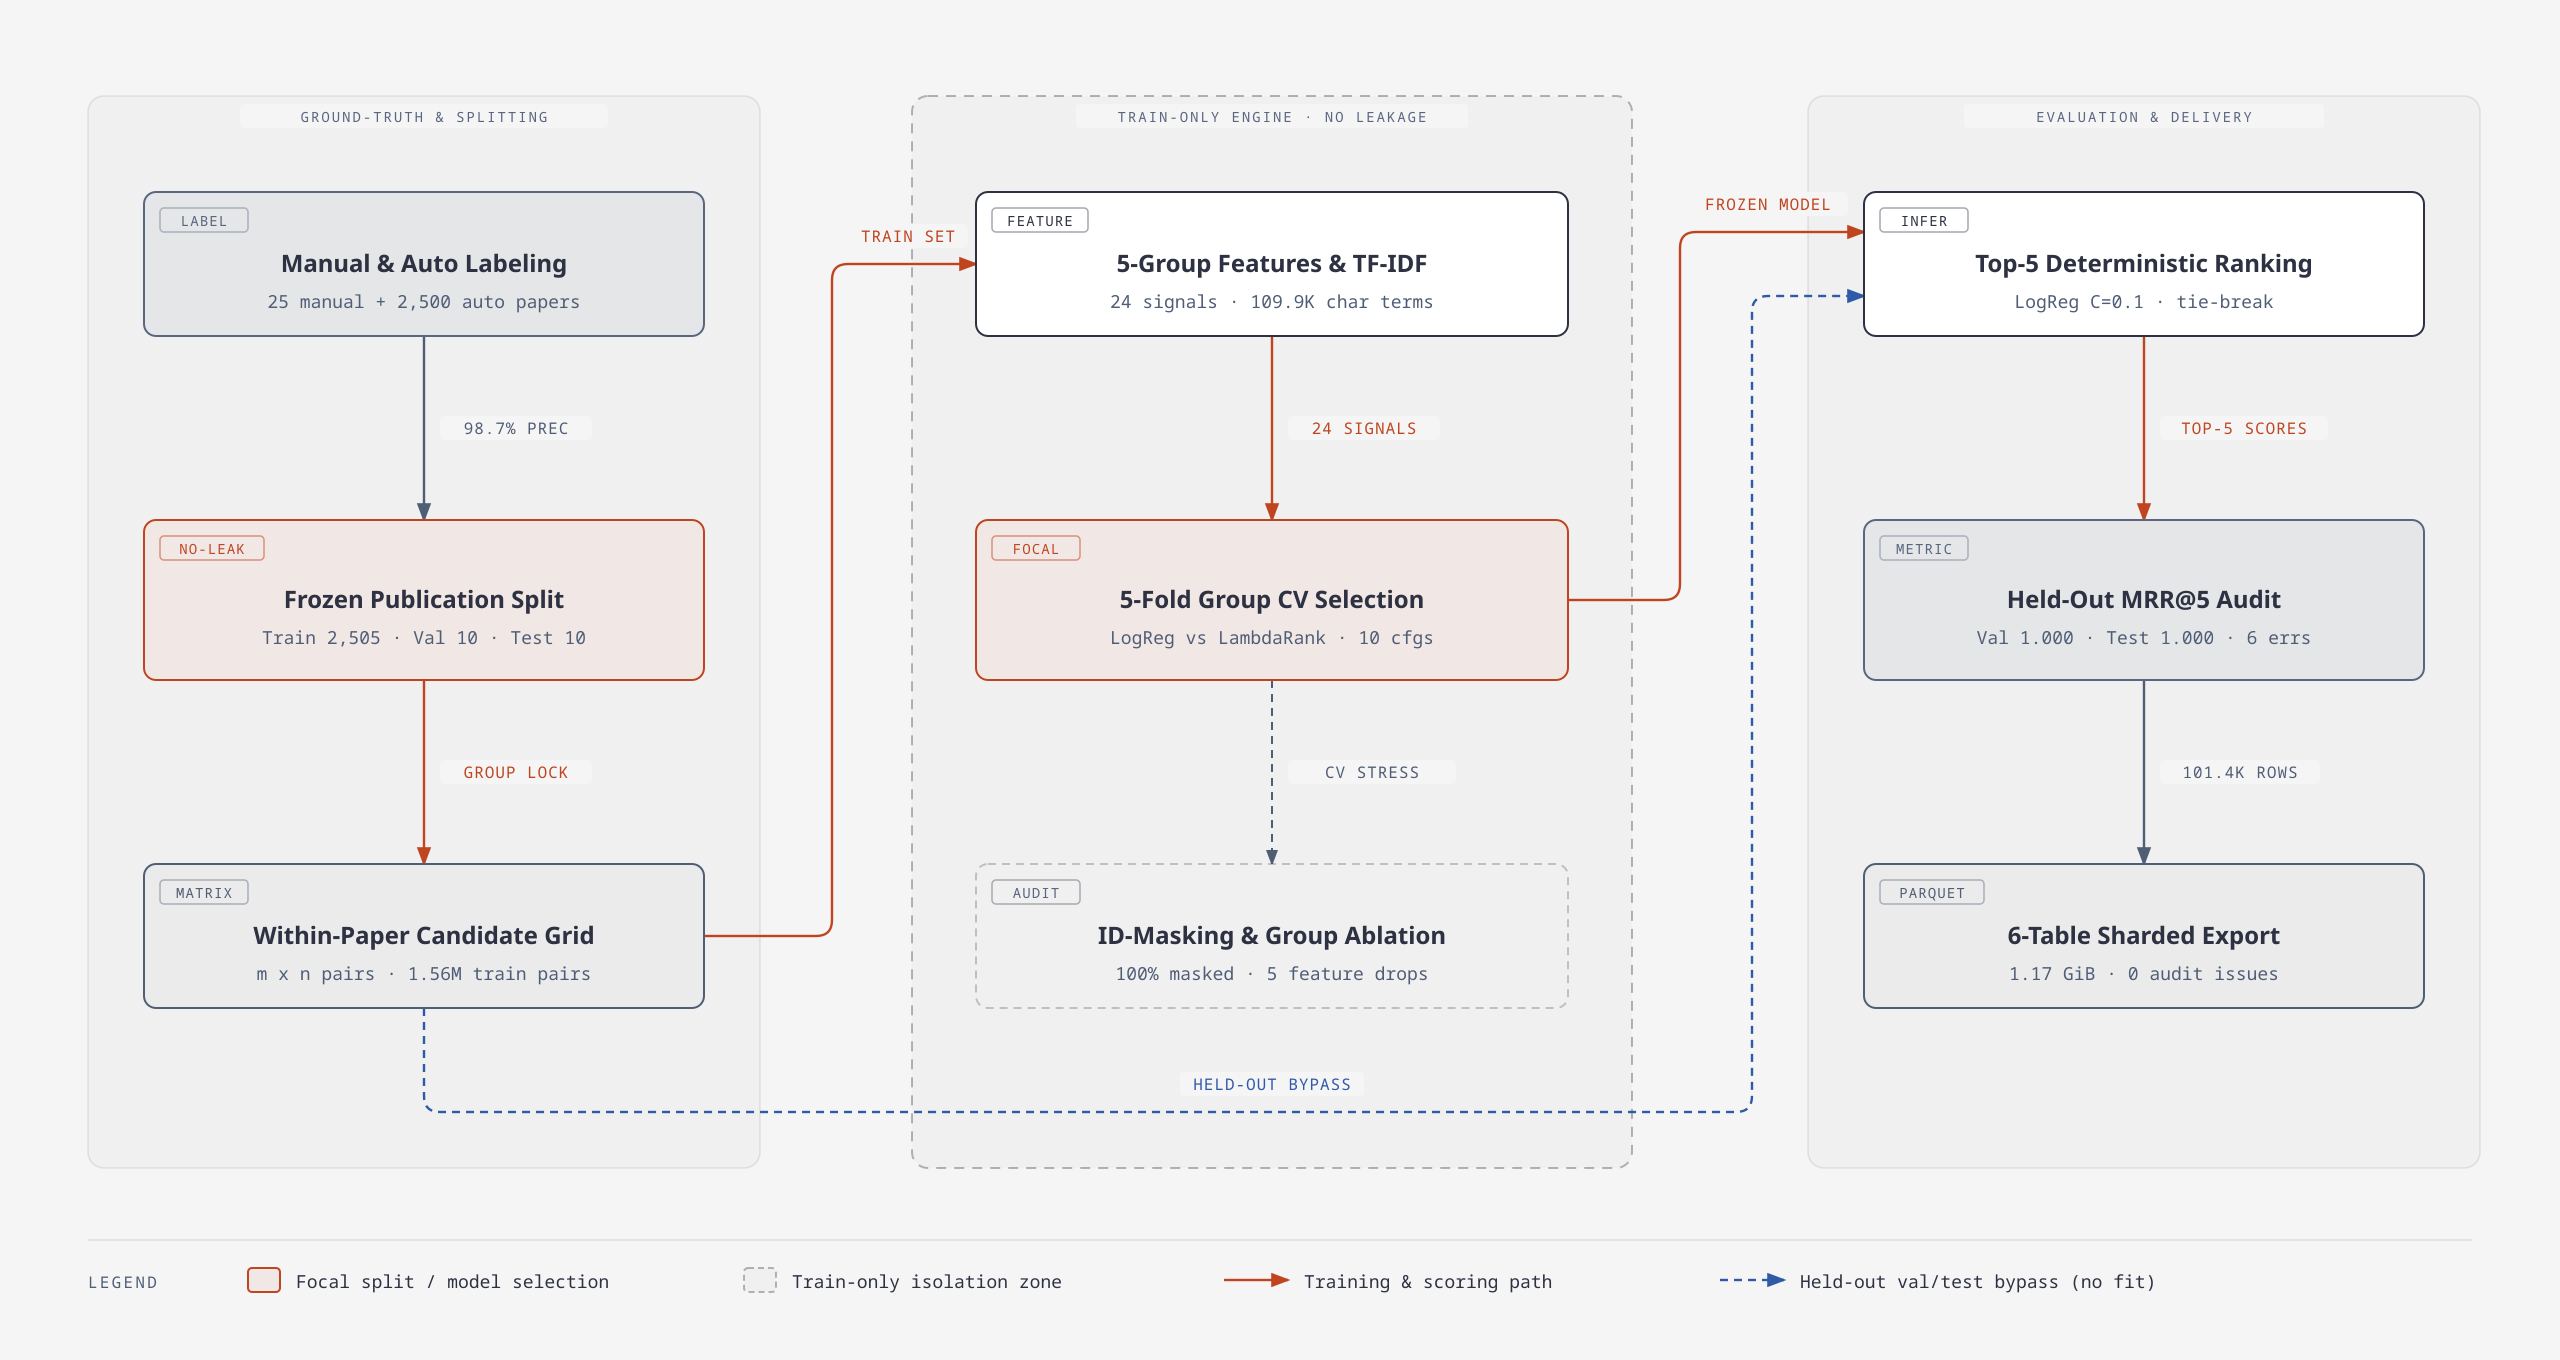
\includegraphics[width=\linewidth]{images/m3_matching_pipeline.png}
    \caption{Kiến trúc luồng xử lý Giai đoạn 3 từ dữ liệu đầu vào, tạo nhãn hai tầng, trích xuất 24 đặc trưng năm nhóm đến kiểm định chéo nhóm và xuất bản sáu bảng dữ liệu}
    \label{fig:m3_matching_pipeline}
\end{figure}

\subsection{Tiền xử lý văn bản và thiết kế hệ thống 24 đặc trưng}

Một quyết định thiết kế quan trọng của giai đoạn học máy là xây dựng dây chuyền chuẩn hóa văn bản độc lập hoàn toàn với bộ quy tắc gán nhãn tự động nhằm giảm thiểu rủi ro rò rỉ định kiến quy tắc vào biểu diễn đầu vào của mô hình. Trước khi tính toán bất kỳ độ đo tương đồng nào, tiêu đề của cả mục BibTeX lẫn tài liệu tham khảo arXiv đều đi qua chuỗi làm sạch gồm loại bỏ dấu phụ và lệnh ký tự Hy Lạp LaTeX, phân rã chuẩn hóa Unicode NFKD, chuyển về chữ thường và lọc từ dừng tiếng Anh thông dụng. Khác với nhiều bộ tiền xử lý ngôn ngữ tự nhiên phổ thông vốn loại bỏ mọi từ quá ngắn, bộ tách từ ở đây giữ nguyên toàn bộ ký hiệu toán học đơn ký tự và chữ số nhằm bảo toàn thông tin định danh đặc thù trong tiêu đề khoa học như tên đồ thị, nhóm đối xứng hay mức năng lượng. Đối với siêu dữ liệu tác giả, bộ phân tích họ tách riêng phần họ chuẩn hóa đồng thời xử lý đúng các hậu tố học thuật và tên các tổ chức hợp tác lớn trong vật lý năng lượng cao hay thiên văn học. Song song đó, bộ trích xuất mã định danh chỉ nhận diện mã arXiv khi đi kèm tiền tố ngữ cảnh tường minh của arXiv để tránh nhầm lẫn với số trang hay định danh tạp chí, còn năm công bố được trích xuất thống nhất về dạng số nguyên bốn chữ số.

Trên nền văn bản đã chuẩn hóa, mỗi cặp ứng viên $(e_i, r_j)$ trong cùng bài báo $p$ được mã hóa thành một vector gồm $24$ đặc trưng phân bổ vào năm nhóm ngữ nghĩa có tính bổ trợ chặt chẽ. Nhóm thứ nhất gồm $3$ đặc trưng định danh phản ánh trực tiếp trạng thái khớp mã arXiv: chỉ báo trùng khớp tuyệt đối mã arXiv giữa mục BibTeX và ứng viên, chỉ báo mục BibTeX có chứa mã arXiv tường minh, và chỉ báo xung đột mã định danh khi mục trích dẫn mang một mã arXiv xác định nhưng khác với mã của ứng viên đang xét. Nhóm thứ hai gồm $9$ đặc trưng từ vựng và tiểu từ trên tiêu đề nhằm bắt giữ đồng thời độ tương đồng cấp từ, độ bao hàm bất đối xứng khi một bên bị cắt ngắn và độ bền vững trước sai khác chính tả hay dấu gạch nối. Gọi $W_e$ và $W_r$ lần lượt là tập từ chuẩn hóa của tiêu đề mục BibTeX và ứng viên arXiv, ba độ đo tập hợp nền tảng gồm chỉ số Jaccard $J(W_e, W_r) = |W_e \cap W_r| / |W_e \cup W_r|$, tỷ lệ bao hàm chiều mục trích dẫn trong ứng viên $|W_e \cap W_r| / |W_e|$ và chiều ngược lại $|W_e \cap W_r| / |W_r|$. Bên cạnh hai độ tương đồng mờ theo tập từ và chuỗi con cục bộ, nhóm này bổ sung độ tương đồng cosin trên không gian vector TF-IDF $n$-gram ký tự độ dài $3$ đến $5$ với từ điển $109{,}864$ mục chỉ được khớp duy nhất trên tiêu đề tập huấn luyện để triệt tiêu rò rỉ thống kê. Ba đặc trưng còn lại của nhóm Tiêu đề là tỷ số độ dài tập từ giữa hai tiêu đề, chỉ báo trùng khớp chính xác tiêu đề chuẩn hóa và chỉ báo thiếu trường tiêu đề.

Ba nhóm đặc trưng còn lại cung cấp thông tin phân biệt ở tầng siêu dữ liệu đồng xuất hiện và cấu trúc cạnh tranh nội bài báo, giữ vai trò quyết định khi tiêu đề bị cắt xén hoặc nhiều bài báo cùng chuỗi sở hữu tiêu đề gần như trùng khít. Nhóm thứ ba gồm $4$ đặc trưng tác giả đo lường chỉ báo trùng khớp họ tác giả đầu tiên, chỉ số Jaccard trên tập họ tác giả, số lượng họ tác giả giao nhau tuyệt đối và chỉ báo thiếu trường tác giả. Việc giữ song song số lượng tác giả trùng lặp tuyệt đối bên cạnh chỉ số Jaccard đặc biệt hữu ích đối với các công trình hợp tác đông tác giả, nơi tỷ lệ Jaccard bị pha loãng khi tệp BibTeX rút gọn danh sách tác giả. Nhóm thứ tư gồm $3$ đặc trưng thời gian biểu diễn độ trễ công bố có dấu $\Delta y = y_e - y_r$, chỉ báo nằm trong ngưỡng sai lệch một năm $|\Delta y| \le 1$ và chỉ báo thiếu năm công bố. Giữ lại dấu của $\Delta y$ thay vì chỉ lấy giá trị tuyệt đối phản ánh đúng cơ chế xuất bản học thuật khi bản thảo nộp lên arXiv ở năm $y_r$ thường được đăng chính thức trên tạp chí hoặc hội nghị ở cùng năm hoặc năm kế tiếp ($\Delta y \in \{0, 1\}$). Nhóm thứ năm gồm $5$ đặc trưng cạnh tranh nội mục và liên mục trong bài báo $p$: thứ hạng tương đồng tiêu đề của ứng viên $r_j$ trong mục $e_i$, khoảng cách điểm so với ứng viên đứng đầu $g_{ij} = \max_{k} s(e_i, r_k) - s(e_i, r_j)$, điểm chuẩn hóa nội nhóm $z_{ij} = (s(e_i, r_j) - \mu_i) / \sigma_i$, chỉ báo song ánh tốt nhất hai chiều (bằng $1$ khi $r_j$ là ứng viên tiêu đề cao nhất của $e_i$ đồng thời $e_i$ là mục phù hợp nhất của $r_j$) và kích thước tập ứng viên $n_p$.

\begin{table}[htbp]
    \centering
    \scriptsize
    \renewcommand{\arraystretch}{1.14}
    \begin{tabularx}{\textwidth}{l X r r r l}
        \toprule
        \textbf{Nhóm} & \textbf{Đặc trưng (24 đặc trưng thuộc 5 nhóm)} & \textbf{TB (+)} & \textbf{TB (--)} & \textbf{AUC} & \textbf{Trọng số LR / Gain LGB nổi bật} \\
        \midrule
        \multirow{3}{*}{Định danh (3)}
            & Trùng khớp trực tiếp mã định danh arXiv & $0.2168$ & $0.0000$ & $0.6084$ & LR: $+3.244$; LGB: $35{,}143$ \\
            & Mục BibTeX có mã định danh arXiv tường minh & $0.2168$ & $0.2075$ & -- & LR: $-0.890$ \\
            & Xung đột mã định danh với ứng viên & $0.0000$ & $0.2075$ & $0.3962$ & LR: $-1.453$; LGB: $2{,}866$ \\
        \midrule
        \multirow{9}{*}{Tiêu đề (9)}
            & Chỉ số Jaccard tập từ tiêu đề $J(W_e, W_r)$ & $0.9788$ & $0.0538$ & $\mathbf{0.9964}$ & LR: $+1.882$; LGB: $1{,}842$ \\
            & Độ bao hàm từ tiêu đề mục trong ứng viên & $0.9826$ & $0.0958$ & $0.9954$ & LR: $-1.512$ \\
            & Độ bao hàm từ tiêu đề ứng viên trong mục & $0.9895$ & $0.0963$ & $0.9962$ & LGB: $2{,}269$ \\
            & Tương đồng mờ theo tập từ tiêu đề & $0.9951$ & $0.4462$ & $0.9950$ & -- \\
            & Tương đồng mờ theo chuỗi con cục bộ & $0.9948$ & $0.4759$ & $0.9956$ & -- \\
            & Cosin TF-IDF $n$-gram ký tự ($3$--$5$) & $0.9871$ & $0.1102$ & $0.9957$ & LR: $+1.515$ \\
            & Tỷ số độ dài tập từ hai tiêu đề & $0.9864$ & $0.7094$ & $0.9207$ & LR: $+0.885$; LGB: $2{,}428$ \\
            & Trùng khớp chính xác tiêu đề chuẩn hóa & $0.9431$ & $0.0000$ & $0.9715$ & LR: $+1.010$ \\
            & Chỉ báo thiếu trường tiêu đề & $0.0000$ & $0.0000$ & -- & -- \\
        \midrule
        \multirow{4}{*}{Tác giả (4)}
            & Trùng khớp họ tác giả đầu tiên & $0.9650$ & $0.0144$ & $0.9753$ & LGB: $1{,}469$ \\
            & Chỉ số Jaccard tập họ tác giả & $0.9086$ & $0.0234$ & $\mathbf{0.9862}$ & LGB: $697$ \\
            & Số lượng họ tác giả trùng lặp & $5.419$ & $0.262$ & $0.9722$ & -- \\
            & Chỉ báo thiếu danh sách tác giả & $0.0020$ & $0.0024$ & -- & -- \\
        \midrule
        \multirow{3}{*}{Thời gian (3)}
            & Chênh lệch năm công bố có dấu $\Delta y$ & $0.411$ & $0.447$ & -- & LGB: $1{,}759$ \\
            & Chỉ báo sai lệch trong vòng một năm $|\Delta y| \le 1$ & $0.9193$ & $0.3293$ & $0.7950$ & LR: $+0.841$ \\
            & Chỉ báo thiếu trường năm công bố & $0.0097$ & $0.0061$ & -- & -- \\
        \midrule
        \multirow{5}{*}{Cạnh tranh (5)}
            & Thứ hạng tiêu đề trong nội bộ mục truy vấn & $1.096$ & $35.146$ & $0.9978^*$ & LGB: $\mathbf{3{,}309{,}532}$ \\
            & Khoảng cách điểm so với ứng viên đứng đầu $g_{ij}$ & $0.0007$ & $0.5502$ & $\mathbf{0.9989^*}$ & LR: $\mathbf{-3.317}$; LGB: $160{,}866$ \\
            & Điểm chuẩn hóa nội mục $z_{ij}$ & $+4.339$ & $-0.098$ & $0.9956$ & LR: $+1.167$; LGB: $1{,}085$ \\
            & Tín hiệu song ánh tốt nhất hai chiều & $0.9907$ & $0.0012$ & $0.9947$ & -- \\
            & Kích thước tập ứng viên của bài báo $n_p$ & $45.49$ & $68.60$ & -- & LR: $-1.957$ \\
        \bottomrule
    \end{tabularx}
    \caption[Thống kê phân tách 24 đặc trưng trên 1{,}561{,}952 cặp ứng viên huấn luyện]{Thống kê phân tách 24 đặc trưng trên $1{,}561{,}952$ cặp ứng viên huấn luyện (TB (+)/(--): trung bình lớp dương/âm; dấu $^*$ biểu thị ROC-AUC đảo chiều $1 - \text{AUC}$ cho các đặc trưng có tương quan nghịch với xác suất khớp; ký hiệu ``--'' ứng với các hệ số phụ hoặc đa cộng tuyến không thuộc nhóm dẫn đầu).}
    \label{tab:m3_features}
\end{table}

Thống kê thực nghiệm trên toàn bộ $1{,}561{,}952$ cặp ứng viên huấn luyện tại Bảng~\ref{tab:m3_features} minh họa mức độ phân tách rõ rệt của hệ thống đặc trưng thiết kế, đồng thời làm nổi bật sự khác biệt trong cách khai thác tín hiệu giữa mô hình tuyến tính và mô hình cây quyết định. Xét đơn biến theo chỉ số ROC-AUC, hai đặc trưng cạnh tranh nội nhóm dẫn đầu tuyệt đối với khoảng cách so với ứng viên đứng đầu đạt $0.9989$ (đảo chiều từ $0.0011$, trung bình $0.0007$ ở lớp dương so với $0.5502$ ở lớp âm) và thứ hạng tiêu đề nội mục đạt $0.9978$ (đảo chiều từ $0.0022$, trung bình $1.096$ so với $35.146$). Theo sát ngay sau là nhóm đặc trưng tiêu đề và tác giả, nổi bật là chỉ số Jaccard tập từ ($0.9964$), độ bao hàm ứng viên trong mục ($0.9962$), cosin TF-IDF ký tự ($0.9957$) và Jaccard họ tác giả ($0.9862$). Ở Hồi quy Logistic chuẩn hóa, khoảng cách so với ứng viên đứng đầu nhận trọng số âm mạnh nhất ($-3.317$) và trùng khớp mã định danh nhận trọng số dương lớn nhất ($+3.244$), trong khi xung đột mã định danh mang trọng số phạt $-1.453$ và kích thước tập ứng viên mang trọng số hiệu chỉnh nền $-1.957$. Đáng chú ý, độ bao hàm chiều mục trong ứng viên nhận dấu âm ($-1.512$) bên cạnh Jaccard ($+1.882$) và TF-IDF ký tự ($+1.515$) như một thành phần cân bằng đa cộng tuyến nhằm phạt các tiêu đề quá ngắn vô tình lọt trọn vào một tiêu đề dài hơn. Ngược lại, ở mô hình LightGBM LambdaRank, thứ hạng tiêu đề nội mục chiếm ưu thế áp đảo về độ lợi chia nhánh ($3{,}309{,}532$), theo sau là khoảng cách so với ứng viên đứng đầu ($160{,}866$) và trùng khớp mã định danh ($35{,}143$), cho thấy cấu trúc cây phân tầng đặt thứ hạng nội nhóm làm trục phân tách gốc rồi tinh chỉnh các ca tranh chấp bằng mã định danh, tỷ số độ dài tiêu đề, chênh lệch năm có dấu và họ tác giả đầu tiên.

\subsection{Quy trình huấn luyện, kiểm định chéo, kịch bản che mã định danh và kết quả MRR@5}

Hiệu năng xếp hạng của toàn bộ mô hình được đo lường bằng chỉ số Thứ hạng nghịch đảo trung bình trong tốp năm ứng viên đầu tiên ($\text{MRR@5}$)~\cite{craswell2009}, định nghĩa trên tập truy vấn có nhãn đúng $Q$ theo Công thức~\eqref{eq:mrr5}:
\begin{equation}
    \text{MRR@5} = \frac{1}{|Q|} \sum_{i=1}^{|Q|} \mathbb{I}(\text{rank}_i \le 5)\,\frac{1}{\text{rank}_i},
    \label{eq:mrr5}
\end{equation}
trong đó $\text{rank}_i \in \{1, \dots, n_p\}$ là vị trí của tài liệu tham khảo đích $r^*_i$ sau khi sắp xếp toàn bộ ứng viên của bài báo $p$ theo điểm dự đoán giảm dần, còn hàm chỉ thị $\mathbb{I}(\text{rank}_i \le 5)$ gán giá trị $0$ cho mọi truy vấn có đích đúng rơi ra ngoài năm hạng đầu. Tuân thủ quy ước đánh giá thống nhất của học phần~\cite{hcmus_intro_ds}, mẫu số $|Q|$ bao gồm tất cả các mục BibTeX đã xác minh có tài liệu tham khảo đích tồn tại trong kho arXiv của bài báo ($35{,}373$ truy vấn toàn cục). Trong khi đó, bảng kết quả dự đoán phát hành vẫn cung cấp đầy đủ năm ứng viên xếp hạng cao nhất cho toàn bộ $101{,}441$ mục thuộc tập đối sánh và để trống trường mã đích chuẩn đối với các mục không có đích khớp hoặc chưa rà soát. Xuyên suốt quy trình huấn luyện, nguyên tắc chống rò rỉ dữ liệu được áp dụng tuyệt đối ở mọi tầng xử lý. Bộ biến đổi TF-IDF $n$-gram ký tự, bộ chuẩn hóa tỷ lệ đặc trưng và các tham số mô hình đều chỉ được khớp trên tập huấn luyện (hoặc từng nếp huấn luyện trong kiểm định chéo), còn tập kiểm tra $10$ bài báo ($528$ truy vấn) bị niêm phong hoàn toàn cho đến sau khi chốt mô hình duy nhất.

Quá trình lựa chọn mô hình triển khai kiểm định chéo năm nếp phân nhóm theo bài báo (5-fold Group K-Fold) trên $2{,}505$ bài báo huấn luyện ($34{,}334$ truy vấn), khảo sát lưới $10$ cấu hình gồm $3$ mức điều chuẩn của Hồi quy Logistic ($C \in \{0.1, 1.0, 10.0\}$) và $2$ mức dung lượng của LightGBM LambdaRank ($15$ và $31$ lá). Mỗi mô hình được thử nghiệm song song ở hai chế độ không tăng cường và có tăng cường dữ liệu che mã định danh tất định với xác suất $50\%$, tức cố ý ẩn nhóm đặc trưng mã arXiv trên một nửa truy vấn huấn luyện để buộc mô hình học sâu hơn từ tiêu đề, tác giả và năm công bố. Ngoài kịch bản đánh giá bình thường, mọi cấu hình đều phải trải qua bài kiểm tra áp lực che $100\%$ mã định danh nhằm đo khả năng tổng quát hóa khi gặp các mục BibTeX hoàn toàn thiếu mã arXiv. Trên tập con $1{,}014$ truy vấn thủ công nằm trong phần huấn luyện, cả $10$ cấu hình đều đạt điểm tuyệt đối $1.0000$ ở cả hai kịch bản, qua đó kích hoạt quy tắc phân giải hòa theo độ phức tạp ưu tiên mô hình tuyến tính gọn nhẹ và điều chuẩn mạnh nhất là Hồi quy Logistic ($C = 0.1$, không tăng cường). Khi mở rộng đánh giá sang toàn bộ $34{,}334$ truy vấn kiểm định chéo như tổng hợp tại Bảng~\ref{tab:m3_results}, Hồi quy Logistic ($C = 0.1$) dẫn đầu điểm kiểm định chéo bình thường ở mức $0.999898$. Đáng chú ý, việc bật tăng cường che $50\%$ mã định danh giúp Hồi quy Logistic ($C = 10.0$) nâng điểm kiểm định chéo che mã từ $0.997018$ lên $0.998662$, và đặc biệt đẩy LightGBM LambdaRank ($31$ lá) đạt $0.999100$---cắt giảm xấp xỉ $70\%$ tỷ lệ sai số xếp hạng trong điều kiện vắng mã định danh mà vẫn duy trì điểm bình thường ở mức $0.999869$.

\begin{table}[htbp]
    \centering
    \scriptsize
    \renewcommand{\arraystretch}{1.18}
    \begin{tabularx}{\textwidth}{X c c c c c}
        \toprule
        \textbf{Mô hình / Cấu hình đánh giá} & \textbf{CV Thường} & \textbf{CV Che ID} & \textbf{Valid ($n=511$)} & \textbf{Test ($n=528$)} & \textbf{Toàn cục ($35{,}373$)} \\
        \midrule
        Đường cơ sở (tương đồng tập từ tiêu đề) & -- & -- & $0.9780$ ($0.9741^\dagger$) & $0.9981$ ($0.9977^\dagger$) & $0.9848$ ($905$ lỗi) \\
        \midrule
        \textbf{LR ($C=0.1$, không tăng cường) [Đã chọn]} & $\mathbf{0.999898}$ & $0.997018$ & $\mathbf{1.0000}$ & $\mathbf{1.0000}$ & $\mathbf{0.999901}$ ($6$ lỗi) \\
        LR ($C=10.0$, tăng cường che $50\%$ ID) & $0.999840$ & $0.998662$ & -- & -- & -- \\
        LightGBM LambdaRank ($15$ lá, không tăng cường) & $0.999869$ & $0.997054$ & -- & -- & -- \\
        LightGBM LambdaRank ($31$ lá, tăng cường che $50\%$ ID) & $0.999869$ & $\mathbf{0.999100}$ & $\mathbf{1.0000}$ & $\mathbf{1.0000}$ & -- \\
        \bottomrule
    \end{tabularx}
    \caption[So sánh chỉ số MRR@5 giữa đường cơ sở và các cấu hình học máy]{So sánh chỉ số MRR@5 giữa đường cơ sở và các cấu hình học máy trên kiểm định chéo $5$ nếp ($n=34{,}334$), tập kiểm định, tập kiểm tra và toàn bộ kho nhãn (giá trị mang dấu $^\dagger$ biểu thị điểm riêng trên phân tập nhãn thủ công của đường cơ sở; trên Valid và Test, mô hình được chọn đạt $1.0000$ ở cả chế độ thường lẫn che $100\%$ mã định danh).}
    \label{tab:m3_results}
\end{table}

Trên hai tập đánh giá độc lập, mô hình Hồi quy Logistic được chọn mang lại mức cải thiện rõ rệt so với đường cơ sở chỉ dựa trên tương đồng tập từ tiêu đề. Đường cơ sở đạt MRR@5 bằng $0.9780$ trên tập kiểm định ($0.9741$ trên phần thủ công và $1.0000$ trên phần tự động; tỷ lệ khớp đúng hạng nhất $95.69\%$, tốp ba $99.80\%$ và tốp năm $100.0\%$) và đạt $0.9981$ trên tập kiểm tra ($0.9977$ trên phần thủ công và $1.0000$ trên phần tự động; hạng nhất $99.62\%$, tốp ba và tốp năm $100.0\%$). Khi mở rộng ra toàn bộ $35{,}373$ truy vấn, hạn chế của tiêu chí chỉ xét tiêu đề bộc lộ rõ với điểm MRR@5 dừng ở $0.9848$ kèm $905$ trường hợp trượt khỏi hạng nhất, bao gồm $669$ trường hợp ở hạng $2$, $73$ ở hạng $3$, $16$ ở hạng $4$, $19$ ở hạng $5$ và $128$ trường hợp rơi hoàn toàn khỏi tốp năm. Ngược lại, mô hình Hồi quy Logistic ($C=0.1$) đạt MRR@5 tuyệt đối $1.0000$ trên cả $511$ truy vấn kiểm định lẫn $528$ truy vấn kiểm tra với $0$ sai số, đồng thời bảo toàn trọn vẹn mức $1.0000$ ngay cả khi che $100\%$ mã arXiv. Cấu hình LightGBM LambdaRank ($31$ lá, có tăng cường che mã) cũng tái lập mức $1.0000$ tương đương trên cả hai phân vùng độc lập này. Tính trên toàn bộ $35{,}373$ truy vấn, mô hình được chọn đạt MRR@5 bằng $0.999901$ với tỷ lệ khớp đúng hạng nhất lên đến $99.983\%$ và tỷ lệ trong tốp ba cũng như tốp năm đạt $99.997\%$, chỉ ghi nhận đúng $6$ bất đồng trên toàn bộ kho dữ liệu (gồm $5$ trường hợp ở hạng $2$ và $1$ trường hợp ngoài tốp năm, toàn bộ đều nằm trong phần tự động của tập huấn luyện).

\begin{figure}[htbp]
    \centering
    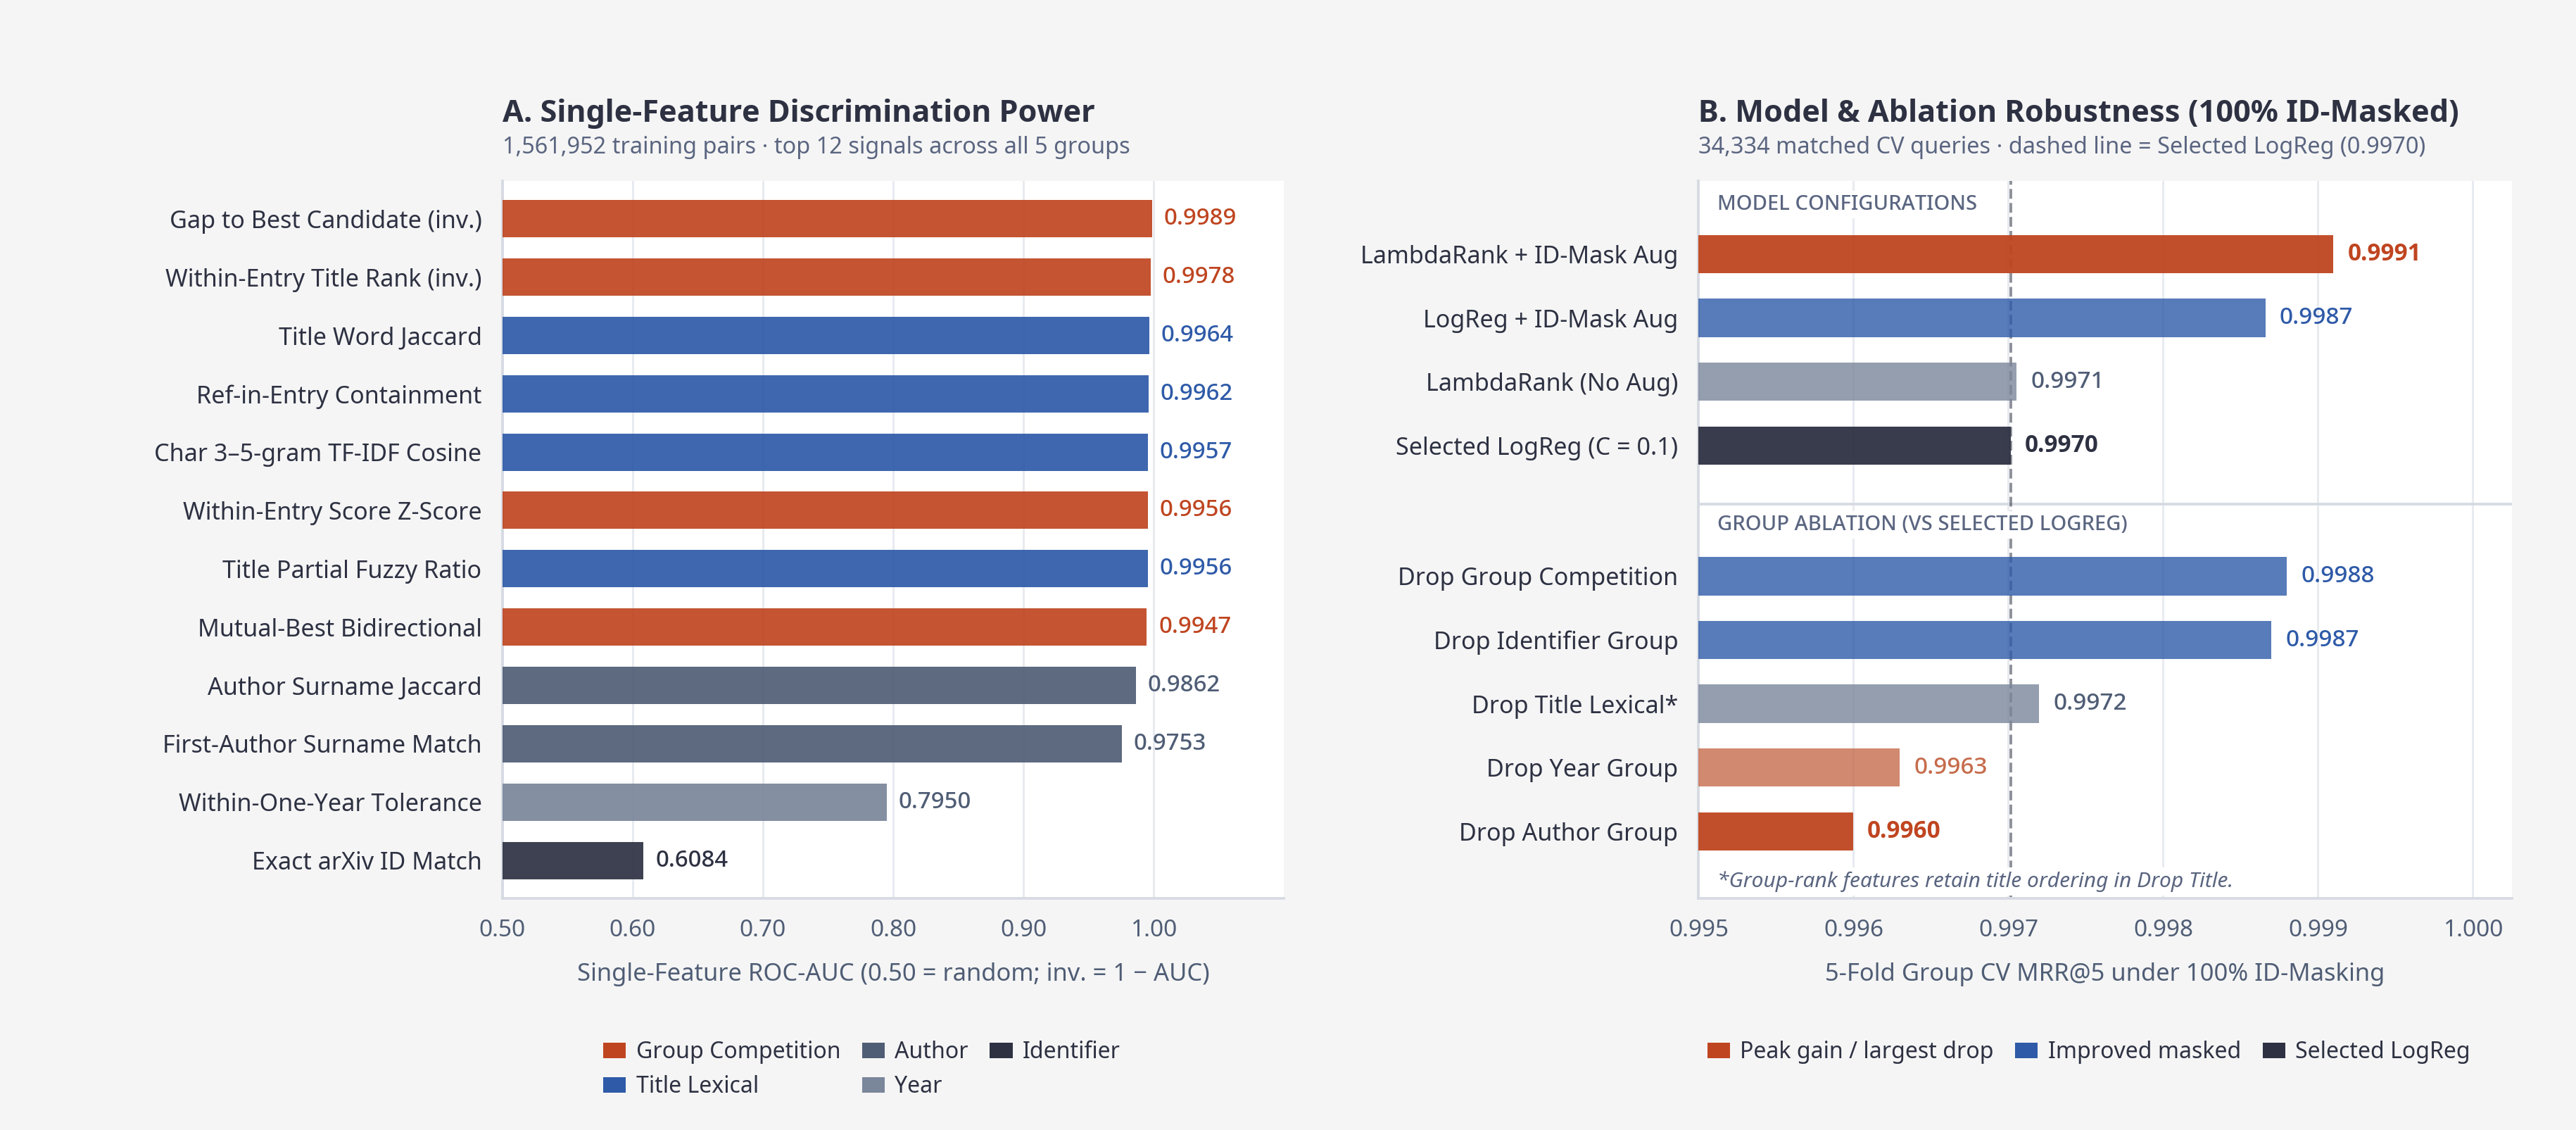
\includegraphics[width=\linewidth]{images/m3_feature_ablation.png}
    \caption[Năng lực phân tách đặc trưng và thí nghiệm loại trừ nhóm đặc trưng]{Đánh giá năng lực phân tách của các nhóm đặc trưng và kết quả thí nghiệm loại trừ từng nhóm đặc trưng trên kiểm định chéo $5$ nếp ($34{,}334$ truy vấn) dưới hai kịch bản bình thường và che $100\%$ mã định danh.}
    \label{fig:m3_feature_ablation}
\end{figure}

Để kiểm chứng đóng góp biên thực sự của từng nhóm tín hiệu, nhóm tiến hành nghiên cứu loại trừ lần lượt từng nhóm đặc trưng trên toàn bộ $34{,}334$ truy vấn kiểm định chéo như minh họa tại Hình~\ref{fig:m3_feature_ablation}. So với cấu hình đầy đủ đạt $0.9999$ ở chế độ bình thường và $0.9970$ ở chế độ che mã định danh, việc loại bỏ nhóm Tác giả gây sụt giảm mạnh nhất dưới kịch bản che mã xuống còn $0.9960$, theo sát ngay sau là việc loại bỏ nhóm Thời gian làm giảm điểm che mã xuống $0.9963$. Kết quả thực nghiệm này chứng minh siêu dữ liệu tác giả và độ trễ năm công bố đóng vai trò phân giải chủ lực khi các mục trích dẫn thiếu mã arXiv. Hai phát hiện nghịch trực giác nhưng nhất quán về mặt cơ chế cũng xuất hiện rõ ràng trong bảng loại trừ: khi loại bỏ nhóm Định danh ngay từ lúc huấn luyện, điểm bình thường giảm nhẹ về $0.9987$ nhưng điểm che mã lại tăng từ $0.9970$ lên $0.9987$ vì mô hình buộc phải phân bổ trọng số đồng đều cho văn bản và siêu dữ liệu thay vì ỷ lại vào mã arXiv. Tương tự, việc loại bỏ nhóm Cạnh tranh giúp điểm che mã tăng lên $0.9988$ do hạn chế hiện tượng quá phụ thuộc vào thứ hạng tiêu đề thô trong các tình huống tiêu đề bị cắt ngắn. Cần ghi nhận một điểm tinh tế về phương pháp luận ở nhánh loại trừ nhóm Tiêu đề ($0.9992$ bình thường, phân tập thủ công giảm về $0.9992$, và $0.9972$ che mã): do các đặc trưng thứ hạng, khoảng cách tốt nhất và điểm chuẩn hóa trong nhóm Cạnh tranh vẫn được tính từ điểm tương đồng tiêu đề gốc, thông tin thứ tự tiêu đề vẫn gián tiếp lưu lại trong biểu diễn sau khi rút nhóm Tiêu đề.

Về chi phí tính toán và kiểm chứng xuất bản, toàn bộ dây chuyền Giai đoạn 3 cho cả năm thành viên hoàn tất trọn vẹn trên $2$ luồng CPU trong tổng thời gian $772.85\text{ s}$ ($12.88\text{ phút}$) với mức tiêu thụ bộ nhớ đỉnh $2{,}393.5\text{ MB}$. Trong tổng thời lượng này, công đoạn huấn luyện và chọn mô hình tiêu tốn $476.26\text{ s}$, phân bổ chủ yếu vào kiểm định chéo $10$ cấu hình trên $5$ nếp ($407.85\text{ s}$) và trích xuất đặc trưng tập huấn luyện ($30.25\text{ s}$), còn bước khớp lại mô hình Hồi quy Logistic cuối cùng chỉ mất đúng $1.81\text{ s}$. Kết quả đầu ra của cả năm thành viên được đóng gói theo định dạng cột Apache Parquet phân mảnh~\cite{apache_parquet} thành sáu bảng chuẩn có tổng dung lượng $1{,}199.45\text{ MiB}$ ($1.171\text{ GiB}$). Cụ thể, kho dữ liệu bao gồm bảng siêu dữ liệu bài báo ($25{,}000$ dòng, $3.73\text{ MiB}$), bảng tài liệu tham khảo ($466{,}763$ dòng, $75.01\text{ MiB}$), bảng phần tử nội dung ($11{,}098{,}189$ dòng, $902.35\text{ MiB}$), bảng quan hệ phân cấp ($16{,}185{,}255$ dòng, $88.50\text{ MiB}$), bảng mục lục BibTeX ($975{,}674$ dòng, $126.41\text{ MiB}$) và bảng kết quả dự đoán đối sánh ($101{,}441$ dòng, $3.44\text{ MiB}$). Toàn bộ bộ dữ liệu phát hành của cả năm thành viên đều vượt qua quy trình kiểm định tự động độc lập về lược đồ cột, tính duy nhất khóa chính, toàn vẹn khóa ngoại liên bảng và quy tắc thứ hạng tốp năm với $0$ lỗi được phát hiện.

\subsection{Phân tích lỗi chuyên sâu trên toàn bộ 35{,}373 truy vấn}

Vì mô hình Hồi quy Logistic được chọn đạt $0$ sai số trên cả hai tập kiểm định độc lập và chỉ tạo ra đúng $6$ bất đồng trên toàn bộ $35{,}373$ truy vấn có nhãn, nhóm có điều kiện thực hiện kiểm định thủ công toàn diện từng trường hợp mà không cần lấy mẫu xấp xỉ. Quy trình rà soát đối chiếu trực tiếp nội dung mục BibTeX gốc, toàn bộ tập ứng viên arXiv của bài báo trích dẫn và bản gốc công trình khoa học tương ứng để xác định nguyên nhân gốc. Kết quả phân loại tổng hợp tại Bảng~\ref{tab:m3_error_forensics} cho thấy toàn bộ $6$ trường hợp bất đồng đều nằm trong phân vùng tự động của tập huấn luyện, trong đó có tới $4$ trường hợp bắt nguồn từ nhiễu nhãn của bộ quy tắc tự động và $1$ trường hợp xuất phát từ lỗi phân tích cú pháp mục tham khảo ngược dòng từ Giai đoạn 2. Chỉ có duy nhất $1$ trong $6$ bất đồng thực sự là sai sót xếp hạng của mô hình học máy, và ngay trong trường hợp đó tài liệu đích vẫn được xếp sát nút ở hạng $2$. Phân rã này chứng tỏ mô hình tuyến tính điều chuẩn mạnh đã không học vẹt các sai sót hệ thống của nhãn giám sát yếu, mà trái lại đã khái quát hóa chính xác hơn chính bộ quy tắc tạo nhãn huấn luyện của nó.

\begin{table}[htbp]
    \centering
    \scriptsize
    \renewcommand{\arraystretch}{1.18}
    \begin{tabularx}{\textwidth}{c p{0.23\textwidth} c X}
        \toprule
        \textbf{TT} & \textbf{Phân loại nguyên nhân gốc} & \textbf{Hạng nhãn} & \textbf{Bản chất kỹ thuật và ứng xử của mô hình học máy} \\
        \midrule
        1 & Nhiễu nhãn tự động (mô hình sửa đúng) & Hạng $2$ & Bài báo về số bão hòa đồ thị $C_6$ ($2021$): quy tắc loại bỏ từ $2$ ký tự làm ghép nhầm vào bài báo $W_4$ ($2025$); mô hình khôi phục đúng bài $C_6$ nhờ trùng cả bốn tác giả. \\
        2 & Nhiễu nhãn tự động (mô hình sửa đúng) & Hạng $2$ & Bài báo ATLAS $7\text{ TeV}$ ($2014$): quy tắc ghép nhầm sang bài ATLAS $8\text{ TeV}$ ($2016$); mô hình chọn đúng bài $2014$ nhờ khớp tác giả đầu và năm công bố dù tiêu đề bị cắt ngắn. \\
        3 & Nhiễu nhãn tự động (mô hình sửa đúng) & Hạng $2$ & Bài báo hố đen siêu đối xứng của Gutowski và Reall ($2004$): quy tắc ghép nhầm sang bài năm $2006$ của nhóm Kunduri--Lucietti--Reall qua một đồng tác giả; mô hình chọn đúng bài $2004$. \\
        4 & Mục không có đích khớp bị gán nhãn sai & Ngoài tốp $5$ & Bài báo mã lượng tử MDS ($2014$) thực tế không nằm trong tập tham khảo arXiv đã thu hoạch; quy tắc gán nhầm vào bài năm $2014$ khác có chung họ tác giả Zhu, còn mô hình bác bỏ ứng viên sai này. \\
        5 & Lỗi phân tích mục tham khảo Giai đoạn 2 & Hạng $2$ & Mục tham khảo dùng ký hiệu gạch ngang lặp tác giả kèm DOI tạp chí thiên văn nhúng mã $2311.03286$ không có tiền tố arXiv tường minh; quy tắc bắt được dãy số trong khi bộ trích xuất học máy bỏ qua và gặp tiêu đề lỗi. \\
        6 & Lỗi xếp hạng thực sự của mô hình & Hạng $2$ & Bài báo năng lượng tối Barrow ($2021$) viết từ ghép liền (``nonflat'') đối đầu bản có gạch nối (``non-flat'') và bài tiền nhiệm ngắn hơn năm $2020$ đạt bao hàm chuỗi con toàn phần; đích đúng vẫn đứng hạng $2$. \\
        \bottomrule
    \end{tabularx}
    \caption{Phân tích nguyên nhân gốc của toàn bộ $6$ trường hợp bất đồng trên tổng số $35{,}373$ truy vấn}
    \label{tab:m3_error_forensics}
\end{table}

Bốn trường hợp đầu tiên minh họa rõ lợi ích của việc kết hợp đa tín hiệu tác giả, thời gian và bảo toàn ký hiệu ngắn thay vì dựa vào ngưỡng quy tắc cứng. Ở trường hợp thứ nhất về bài báo số bão hòa của đồ thị $C_6$ năm $2021$, bộ quy tắc tự động loại bỏ các từ ngắn hai ký tự khiến cả $C_6$ lẫn $W_4$ biến mất khỏi tiêu đề, dẫn tới ghép nhầm vào một công trình năm $2025$ nghiên cứu đồ thị $W_4$. Trái lại, mô hình học máy giữ nguyên ký hiệu ngắn và khai thác sự trùng khớp trọn vẹn của cả bốn tác giả để xếp đúng bài báo năm $2021$ lên hạng nhất. Ở trường hợp thứ hai liên quan đến đo đạc tiết diện toàn phần của thực nghiệm ATLAS tại năng lượng $7\text{ TeV}$ năm $2014$, tiêu đề lưu trên Semantic Scholar bị cắt ngắn làm tầng mờ của bộ quy tắc nghiêng về bài báo ATLAS $8\text{ TeV}$ năm $2016$, trong khi mô hình học máy dựa vào sự trùng khớp chặt giữa tác giả đầu tiên và năm công bố $2014$ để khôi phục chính xác tài liệu đích. Tương tự, ở trường hợp thứ ba về công trình hố đen siêu đối xứng trong không gian năm chiều của Gutowski và Reall năm $2004$, bộ quy tắc tự động bị đánh lừa bởi một đồng tác giả chung và ghép sang bài báo năm $2006$ của Kunduri, Lucietti và Reall, còn mô hình học máy đưa đúng bài báo gốc năm $2004$ lên vị trí dẫn đầu. Ở trường hợp thứ tư---cũng là trường hợp duy nhất nhãn tự động rơi ra ngoài tốp năm---công trình năm $2014$ về mã lượng tử MDS vốn vắng mặt hoàn toàn trong tập tham khảo arXiv của bài báo trích dẫn nhưng bị bộ quy tắc tự động gán nhầm vào một bài báo mã học khác cùng năm có chung họ tác giả Zhu, cho thấy mô hình đã loại trừ đúng ứng viên nhiễu.

Hai trường hợp cuối cùng chỉ ra trực tiếp các giới hạn kỹ thuật cụ thể ở tầng phân tích cú pháp ngược dòng và tiền xử lý từ ghép. Ở trường hợp thứ năm, nguyên nhân nằm hoàn toàn ở đầu vào của Giai đoạn 2: một mục tham khảo nội tuyến trong vật lý thiên văn dùng quy ước gạch ngang thay thế tên tác giả lặp lại đồng thời nhúng mã $2311.03286$ vào trong mã DOI của tạp chí mà không viết từ khóa arXiv tường minh. Vì vậy, bộ quy tắc tự động vẫn bắt được dãy mã số trong khi bộ phân tích học máy nghiêm ngặt bỏ qua chuỗi số thiếu ngữ cảnh và buộc phải xếp hạng dựa trên chuỗi tiêu đề bị hỏng cấu trúc. Chỉ duy nhất trường hợp thứ sáu là sai lầm xếp hạng thực chất của mô hình tuyến tính khi xử lý biến thể chính tả từ ghép. Cụ thể, mục BibTeX trích dẫn công trình năm $2021$ về năng lượng tối toàn ảnh Barrow trong vũ trụ không phẳng bằng cách viết liền không gạch nối (``nonflat''), trong khi siêu dữ liệu Semantic Scholar ghi dạng có gạch nối (``non-flat''), khiến điểm trùng khớp từ vựng bị giảm tương đối so với bài báo tiền nhiệm năm $2020$ có tiêu đề ngắn hơn đạt bao hàm chuỗi con trọn vẹn. Dù chịu bất lợi chính tả này, mô hình vẫn giữ tài liệu đúng năm $2021$ ở vị trí thứ hai sát nút, đưa tỷ lệ sai sót xếp hạng thực chất trên toàn bộ $35{,}373$ truy vấn về đúng $1/35{,}373$.

\section{Đánh giá hạn chế, giải pháp cải tiến và định hướng hoàn thiện}

\subsection{Hạn chế và giải pháp tối ưu ở giai đoạn thu thập dữ liệu}

Phân tích nhật ký vận hành thực tế trên toàn bộ kho $25{,}000$ bài báo cho thấy điểm nghẽn dễ nhận thấy nhất ở khâu phát hiện bài báo là sự lãng phí yêu cầu mạng tại các dải dữ liệu vắt qua ranh giới tháng. Để thu được đúng $25{,}000$ bài báo hợp lệ, hệ thống đã phải dò tổng cộng $179{,}012$ mã ứng viên trên toàn nhóm. Trong khi ba dải nằm trọn trong một tháng chỉ tốn đúng $5{,}000$ lượt dò mỗi dải ($168.7$ đến $198.9\text{ s}$), hai dải xuyên tháng của Phạm Minh Trọng (tháng $04$--$05/2025$) và Nguyễn Phúc Khang (tháng $06$--$07/2025$) lần lượt tiêu tốn tới $83{,}142$ lượt dò ($3{,}276.5\text{ s}$) và $80{,}870$ lượt dò ($2{,}721.8\text{ s}$). Nguyên nhân trực tiếp là dãy số thứ tự hàng tháng của arXiv luôn dừng thấp hơn rất nhiều so với trần năm chữ số $99{,}999$, khiến chiến lược quét tuần tự phải đi qua đúng $154{,}012$ mã trống ở phần đuôi tháng trước khi chuyển sang tháng kế tiếp. Giải pháp kỹ thuật triệt để là thay cơ chế quét tuyến tính bằng bước ước lượng ranh giới tháng hai pha gồm nhảy bước lũy thừa kết hợp tìm kiếm nhị phân để xác định chính xác chỉ số bài báo cuối cùng hợp lệ trong tháng đầu tiên trước khi gửi truy vấn thu hoạch siêu dữ liệu theo lô qua giao thức OAI-PMH~\cite{arxiv_api,arxiv_oai_2025}. Cách tiếp cận này hạ số yêu cầu thăm dò ranh giới từ hàng chục nghìn xuống mức $O(\log K)$ (dưới hai mươi lượt kiểm tra tồn tại cho mỗi giao điểm tháng), rút ngắn thời gian dò tìm trên các dải xuyên tháng về ngang bằng các dải nội tháng mà vẫn giữ tính tất định và tuân thủ nghiêm giới hạn tần suất truy cập máy chủ.

Điểm nghẽn thời gian thực thi lớn thứ hai nằm ở công đoạn thu hoạch $466{,}763$ liên kết tài liệu tham khảo arXiv cho $20{,}878$ bài báo trích dẫn từ đồ thị tri thức Semantic Scholar~\cite{kinney2023,ammar2018}, vốn chiếm tỷ trọng chủ đạo trong tổng thời gian chạy $26.02$ đến $35.48\text{ giờ}$ trên Google Colab của từng thành viên. Việc gọi từng bài báo đơn lẻ bằng yêu cầu GET chịu giới hạn tần suất nghiêm ngặt tạo ra độ trễ chờ cộng dồn lớn, đồng thời gây truy vấn lặp lại đối với những công trình nền tảng được trích dẫn hàng trăm lần trong cùng kho $25{,}000$ bài. Chuyển sang kiến trúc thu hoạch theo lô thích ứng qua phương thức POST kết hợp bộ điều tiết thùng thẻ bài động, chỉ quay về truy vấn đơn lẻ cho các bài báo có danh sách tham khảo quá dài bị cắt trang, cùng bộ nhớ đệm cục bộ ánh xạ siêu dữ liệu các mã tham chiếu đã giải mã sẽ cắt giảm đáng kể số vòng gọi mạng. Song song với đó, cơ chế quản lý trạng thái tải mã nguồn cần tách bạch hoàn toàn giữa lỗi định dạng bất khả kháng (chẳng hạn $5.38\%$ đến $7.28\%$ phiên bản chỉ có tệp PDF hoặc định dạng không hỗ trợ, nhất quán với khảo sát quy mô lớn~\cite{ginev2024}) với lỗi tạm thời do giới hạn lưu lượng (HTTP 429) hay sự cố máy chủ (HTTP 5xx) sau khi cạn hạn mức thử lại tức thời. Thay vì chốt sớm phiên bản hết lượt thử lại vào trạng thái không thể xử lý vĩnh viễn, cơ sở dữ liệu điểm phục hồi quan hệ cần đánh dấu rõ cờ có thể thử lại để các lượt quét bù độ trễ dài tự động thu hồi những phiên bản gặp nghẽn mạng nhất thời mà không tải lại các bản không có mã nguồn LaTeX.

Về mặt đo lường hiệu năng và quản trị thực nghiệm, hai khoảng trống quan sát cần được chuẩn hóa để nâng cao tính minh bạch tái lập giữa các phiên chạy. Thứ nhất, số liệu đo trên $167$ phiên chạy Colab tại mốc ngày $06/11/2026$ ghi nhận thời gian xử lý trung bình mỗi bài báo ($10.64$ đến $22.61\text{ s}$) lớn gần gấp đôi trung vị ($4.71$ đến $9.56\text{ s}$). Hiện tượng phình số đo này phát sinh khi phép tính lấy mốc hoàn thành cuối cùng trừ mốc bắt đầu đầu tiên vô tình gộp cả khoảng thời gian nằm chờ trong hàng đợi khi bộ điều phối đa giai đoạn chạy xen kẽ nhiều bài báo. Để tách bạch chi phí tính toán và mạng thực tế khỏi độ trễ xếp hàng, hệ thống đo cần ghi nhận độc lập thời lượng hoạt động của từng công đoạn trên mỗi bài báo rồi cộng dồn làm thời gian thực thi hữu ích, đồng thời báo cáo riêng thời gian lưu trú trong hàng đợi. Thứ hai, các bản ghi chuẩn mốc lịch sử ngày $06/11/2026$ được thu trước khi hệ thống bổ sung xác nhận tự động môi trường không dùng GPU và trước đợt bù đắp tài liệu tham khảo cuối cùng cho ba dải dữ liệu, trong khi nhật ký đo thời gian toàn cục của Giai đoạn 2 vẫn lưu phân tán trên bộ nhớ đám mây ngoài kho lưu trữ nội bộ. Hợp nhất cơ chế ghi nhật ký có cấu trúc cho cả Giai đoạn 1 và Giai đoạn 2 sau bước bù đắp cuối cùng---kèm chứng thực phần cứng CPU, phân rã thời lượng từng công đoạn và chuỗi mẫu bộ nhớ tiến trình theo thời gian---sẽ khép kín chuỗi kiểm toán hiệu năng đầu-cuối trên toàn kho $25{,}000$ bài báo.

\subsection{Hạn chế và giải pháp nâng cao độ chính xác ở giai đoạn phân tích cú pháp}

Quá trình phân tích cú pháp trên $22{,}961$ bài báo ($37{,}967$ phiên bản, đạt $92.84\%$ tổng số $40{,}896$ phiên bản khai báo) đã chuyển đổi $16{,}223{,}222$ lượt xuất hiện phần tử thành $11{,}098{,}189$ phần tử duy nhất (giảm $31.59\%$ nhờ khử trùng lặp liên phiên bản) cùng $16{,}185{,}255$ cạnh quan hệ phân cấp. Tuy nhiên, kiểm tra định tính trên đầu ra cho thấy quy trình chuẩn hóa biểu thức toán học hiện tập trung chủ yếu vào các đoạn văn xuôi thân bài trước khi tách câu, còn công thức nội tuyến nằm trong chú thích hình bảng, ô bảng số liệu và tiêu đề mục lục chưa được chuẩn hóa đồng đều theo cùng một chuẩn. Sự bất đối xứng này khiến những chỉnh sửa nhỏ về cú pháp toán học trong tiêu đề mục hoặc chú thích hình giữa hai phiên bản vẫn làm thay đổi chuỗi văn bản và bỏ lỡ cơ hội khử trùng lặp, đồng thời giảm độ nhất quán khi tìm kiếm biểu thức toán trên $285{,}123$ phần tử hình bảng và $468{,}790$ tiêu đề phân cấp (gồm $184{,}592$ mục lớn, $222{,}075$ tiểu mục và $62{,}123$ tiểu mục cấp ba). Mở rộng đường ống chuẩn hóa toán học áp dụng đồng nhất cho mọi nút văn bản thuộc tiêu đề, chú thích và ô bảng là cải tiến có chi phí tính toán thấp nhưng mang lại hiệu quả trực tiếp cho chất lượng chỉ mục. Song song đó, tầng nhận diện cấu trúc cần mở rộng phạm vi bao phủ sang các môi trường bảng có độ rộng tự co giãn, hình bảng xoay ngang và danh sách mô tả định nghĩa. Việc xử lý tường minh cả các khối công thức đặt ngay sau lệnh ngắt dòng mà không có dòng trống ngăn cách cũng sẽ giúp phân tách sạch $991{,}526$ công thức khối khỏi các câu văn xuôi liền kề.

Ở tầng tách câu, hệ thống sản xuất cho $8{,}634{,}050$ câu duy nhất lựa chọn bộ tách theo quy tắc tất định (đạt $7/12$ trường hợp chẩn đoán khó và $40/40$ bài kiểm tra tương thích) nhằm đảm bảo khởi chạy tức thời không phụ thuộc trọng số ngoài và tái lập hoàn toàn theo từng điểm phục hồi trên Colab. Tuy nhiên, cấu trúc biểu thức chính quy kèm danh mục hai mươi từ viết tắt vẫn phát sinh lỗi cắt câu sớm khi gặp chữ cái viết tắt tên tác giả ngắn hoặc có dấu gạch nối, các chuỗi viết tắt học thuật nhiều dấu chấm và cụm trích dẫn dày đặc xen giữa mệnh đề. Ngay cả phương pháp không giám sát NLTK Punkt~\cite{kiss2006} cũng chỉ nhích lên $8/12$ trường hợp chẩn đoán nhưng lại làm giảm tỷ lệ tương thích xuống $38/40$. Thực nghiệm đo chuẩn có kiểm soát trên $100$ bài báo đầu dải ($93$ bài có mã nguồn LaTeX, $7{,}525$ khối văn xuôi, $4{,}803{,}251$ ký tự) mở ra hướng nâng cấp khả thi rõ rệt: mô hình tách câu thống kê nhẹ của spaCy~\cite{spacy} đạt độ chính xác chẩn đoán cao nhất ($10/12$) và khi chạy theo lô kích thước $32$ chỉ tốn $0.104\text{ s}$ mỗi phiên bản với $163.6\text{ MiB}$ bộ nhớ đỉnh (tốc độ $495{,}000$ ký tự mỗi giây). Mức thông lượng này ngoại suy chỉ mất khoảng $1.16\text{ giờ}$ cho toàn bộ $40{,}000$ phiên bản LaTeX, tiết kiệm hơn hai bậc độ lớn so với mô hình nơ-ron đa ngôn ngữ SaT~\cite{frohmann2024} trên CPU đơn lẻ ($153.39\text{ giờ}$ và $1{,}310.1\text{ MiB}$). Do đó, triển khai spaCy chạy theo lô làm bộ đề xuất ranh giới chính kết hợp tầng hậu kiểm tất định cấm cắt ngang bên trong công thức nội tuyến, ngoặc trích dẫn và mẫu viết tắt tên tác giả sẽ đồng thời nâng độ chính xác ngôn ngữ và bảo toàn trọn vẹn tính toàn vẹn cấu trúc toán học trên phần cứng CPU phổ thông.

Một nguồn sai số ngược dòng có tác động trực tiếp đến Giai đoạn 3 nằm ở bước trích xuất mục tham khảo nội tuyến và gộp thư mục BibTeX liên phiên bản. Toàn bộ kho dữ liệu hiện gom được $975{,}674$ mục BibTeX từ $19{,}204$ bài báo ($76.82\%$ tổng số bài) với độ phủ tiêu đề $99.23\%$, năm $98.36\%$ và tác giả $97.03\%$, nhưng vẫn còn $19.17\%$ mục mang loại tổng quát dự phòng thay vì phân loại cụ thể như bài báo tạp chí ($57.93\%$) hay kỷ yếu hội nghị ($18.25\%$). Như phân tích lỗi tại Bảng~\ref{tab:m3_error_forensics} đã chỉ rõ ở trường hợp bất đồng thứ năm, các mục tham khảo nội tuyến trong thiên văn học dùng ký hiệu gạch ngang thay thế tên tác giả lặp lại và nhúng mã arXiv vào trong chuỗi DOI tạp chí khiến bộ phân tích mục nội tuyến hiện tại trích xuất sai trường tác giả và làm nhiễu chuỗi tiêu đề. Để khắc phục triệt để, khối xử lý thư mục cần bổ sung bộ giải tham chiếu tuần tự cho ký hiệu gạch ngang lặp tác giả bằng cách kế thừa danh sách tác giả đã chuẩn hóa từ mục tham khảo liền trước. Tiếp theo, quy tắc gộp liên phiên bản cần áp dụng thứ tự ưu tiên phân loại để loại bài báo tạp chí hoặc kỷ yếu hội nghị tự động thay thế loại dự phòng tổng quát mỗi khi một phiên bản khác bổ sung thông tin tạp chí hay hội nghị (hiện đạt $71.11\%$ độ phủ trường tạp chí). Cuối cùng, bổ sung cơ chế khử trùng lặp mờ đối với biến thể cách viết tên tác giả giữa dạng viết tắt chữ cái đầu và tên đầy đủ sẽ nâng cao tính nhất quán của siêu dữ liệu tác giả cho toàn bộ các tác vụ hạ nguồn.

\subsection{Hạn chế và giải pháp hoàn thiện mô hình đối sánh tài liệu tham khảo}

Mặc dù mô hình Hồi quy Logistic đạt MRR@5 tuyệt đối $1.0000$ trên cả hai tập kiểm định độc lập và chỉ mắc đúng $1$ sai sót xếp hạng thực chất trên toàn bộ $35{,}373$ truy vấn, các kết quả kiểm toán ngược và phân tích lỗi đã chỉ rõ những nút thắt cần xử lý khi mở rộng quy mô. Trước hết, đối với bộ quy tắc gán nhãn tự động tạo dữ liệu giám sát yếu (đạt độ chính xác $98.72\%$ và độ phủ $98.83\%$ trên $25$ bài báo thủ công), toàn bộ $24/24$ lỗi dương tính giả đều tập trung ở tầng mờ thứ ba và $21/22$ lỗi bỏ sót xuất phát từ cơ chế phủ quyết cứng khi vắng mã arXiv. Cải tiến trọng tâm là siết chặt bộ trích xuất định danh bằng yêu cầu ngữ cảnh arXiv tường minh kết hợp chuẩn hóa các mã chuyên ngành kiểu cũ trước năm $2007$ về dạng thống nhất trước khi so sánh, đồng thời điều chỉnh tầng chuẩn hóa tiêu đề của bộ quy tắc để bảo toàn các ký hiệu toán học ngắn hai ký tự như $C_6$ hay $W_4$. Bên cạnh đó, chuyển cơ chế phủ quyết cứng khi mã arXiv vắng mặt thành một mức phạt mềm có thể vượt qua khi tiêu đề, tác giả và năm công bố đạt đồng thuận rất cao sẽ giảm mạnh tỷ lệ bỏ sót mà không làm tăng lỗi ghép nhầm. Về mặt thiết kế thực nghiệm, nghiên cứu loại trừ đặc trưng trong tương lai cần tính lại các đặc trưng cạnh tranh nhóm hoàn toàn trên điểm tổng hợp của các nhóm còn lại khi loại nhóm Tiêu đề nhằm tháo gỡ sự ghép dính phương pháp luận hiện tại. Song song đó, bổ sung tầng chuẩn hóa biến thể từ ghép có và không có dấu gạch nối (đồng nhất các cặp như ``nonflat'' và ``non-flat'') sẽ xử lý trực tiếp nguyên nhân dẫn tới sai số xếp hạng thực chất duy nhất được ghi nhận tại Bảng~\ref{tab:m3_error_forensics}.

Ở cấp độ mô hình hóa bài toán, kiến trúc xếp hạng độc lập theo từng truy vấn hiện tại vẫn còn hai khoảng trống cấu trúc đáng kể khi triển khai trong môi trường sản xuất thực tế. Khoảng trống thứ nhất là khả năng phát hiện tường minh các mục trích dẫn không có bài báo đích trên arXiv: trên tập $101{,}441$ mục BibTeX của nhóm, có tới $65{,}816$ mục không thuộc kho arXiv đã thu hoạch, nhưng mô hình xếp hạng hiện chỉ sắp thứ tự năm ứng viên tốt nhất mà chưa đưa ra quyết định từ chối có kiểm soát độ tin cậy. Khắc phục giới hạn này đòi hỏi huấn luyện thêm nhánh quyết định có hoặc không khớp trên cả các truy vấn toàn âm kết hợp hiệu chỉnh xác suất (như hiệu chỉnh Platt hay hồi quy đơn điệu) để đặt ngưỡng từ chối tối ưu theo tỷ lệ chính xác--độ phủ mong muốn. Khoảng trống thứ hai là tính độc lập giữa các truy vấn trong cùng một bài báo trích dẫn, vốn cho phép hai mục BibTeX khác nhau cùng giành một tài liệu tham khảo arXiv duy nhất làm dự đoán hạng nhất. Áp dụng thuật toán ghép cặp hai phía trọng số cực đại toàn cục (thuật toán Hungary) lên ma trận điểm $m_p \times n_p$ đã hiệu chỉnh của từng bài báo sẽ cưỡng chế ràng buộc tương ứng một-một tự nhiên và tận dụng thông tin loại trừ lẫn nhau. Đáng chú ý hơn, do Giai đoạn 2 đã lưu giữ đầy đủ cấu trúc cây văn bản gắn liền với từng khóa trích dẫn, việc bổ sung kênh đặc trưng ngữ cảnh trích dẫn cục bộ---đo độ tương đồng từ vựng giữa các câu văn bao quanh vị trí trích dẫn trong bài báo với tiêu đề và tóm tắt của tài liệu ứng viên---sẽ cung cấp một nguồn tín hiệu trực giao hoàn toàn mới khi siêu dữ liệu thư mục bị thiếu hoặc cắt xén mà vẫn tuân thủ giới hạn không phụ thuộc mô hình ngôn ngữ lớn bên ngoài.

Kết quả thí nghiệm che mã định danh tại Bảng~\ref{tab:m3_results} và công tác đóng gói phát hành cũng gợi mở lộ trình nâng cấp rõ ràng cho cả lõi mô hình lẫn hạ tầng dữ liệu. Khi áp dụng cho các kho học thuật cũ hơn hoặc các chuyên ngành ít gắn mã arXiv trực tiếp trong tệp thư mục, mô hình xếp hạng theo danh sách LightGBM LambdaRank ($31$ lá) kết hợp tăng cường dữ liệu che $50\%$ mã định danh thể hiện độ bền rõ rệt trước sự vắng mặt của mã định danh. Cụ thể, cấu hình này đã cắt giảm khoảng $70\%$ sai số kiểm định chéo khi che mã (từ $0.9970$ lên $0.9991$) trong khi vẫn giữ trọn mức $1.0000$ trên cả hai tập kiểm định và kiểm tra độc lập. Việc kết hợp có trọng số giữa xác suất đã hiệu chỉnh của Hồi quy Logistic với điểm xếp hạng của LightGBM LambdaRank tăng cường che mã có thể vận hành gọn nhẹ trong cùng giới hạn tài nguyên CPU hiện tại ($12.88\text{ phút}$ chạy toàn nhóm, bộ nhớ đỉnh $2{,}393.5\text{ MB}$ trên $2$ luồng CPU). Về mặt quản trị dữ liệu mở, dù năm bộ dữ liệu cột Parquet phân mảnh theo từng thành viên (tổng dung lượng $1{,}199.45\text{ MiB}$, tương đương $1.171\text{ GiB}$ trên sáu bảng chuẩn) đều đã vượt qua quy trình kiểm định lược đồ, khóa chính, khóa ngoại và quy tắc xếp hạng với $0$ lỗi, kho dữ liệu hiện vẫn phân tán theo năm đầu mục riêng lẻ. Hợp nhất năm kho thành viên dưới một thẻ dữ liệu chung duy nhất của toàn nhóm---đi kèm bảng kiểm kê mã kiểm tra toàn vẹn, chỉ số trùng lặp liên thành viên và tập truy vấn đối chuẩn tái lập---sẽ chuyển hóa năm sản phẩm học phần song song thành một kho chuẩn thống nhất, sẵn sàng phục vụ nghiên cứu phân tích mạng trích dẫn khoa học.

\section{Phân công nhiệm vụ và tổng kết đóng góp}

Đồ án được triển khai xuyên suốt ba giai đoạn kỹ thuật trên kho dữ liệu gồm $25{,}000$ bài báo khoa học arXiv, chia đều thành năm dải mã định danh độc lập với quy mô $5{,}000$ bài báo mỗi thành viên. Mô hình phối hợp của nhóm kết hợp giữa trách nhiệm sở hữu từng công đoạn kỹ thuật cốt lõi và nghĩa vụ vận hành song song trên dải dữ liệu cá nhân, bao gồm thu thập toàn bộ phiên bản nguồn, vận hành phân tích cú pháp, gán nhãn thủ công độc lập đạt chuẩn định mức tối thiểu hai mươi cặp trích dẫn đúng trên mỗi bài báo và kiểm chứng chéo chất lượng dữ liệu trước khi đóng gói phát hành. Bảng~\ref{tab:contribution} tổng hợp phạm vi đảm nhiệm kỹ thuật và đóng góp của từng thành viên trong nhóm ChickenDev qua cả ba cột mốc của đồ án.

\begin{table}[H]
    \centering
    \scriptsize
    \setlength{\tabcolsep}{4pt}
    \renewcommand{\arraystretch}{1.05}
    \begin{tabularx}{\textwidth}{l p{0.17\textwidth} X c}
        \toprule
        \textbf{Họ và tên} & \textbf{Dải dữ liệu} &
        \textbf{Phạm vi kỹ thuật và vận hành đảm nhiệm} & \textbf{Đóng góp} \\
        \midrule
        Phạm Minh Trọng & 2504.17523 -- 2505.00665 \newline (5{,}000 bài)
            & Thiết kế cơ chế dò tìm bài báo theo lô xuyên ranh giới tháng, bộ điều phối tiến trình đa giai đoạn có lưu điểm phục hồi quan hệ và xuất bản giao dịch hai pha ở Giai đoạn 1; xây dựng quy trình tích hợp khử trùng lặp liên phiên bản, lưu trữ cột phân mảnh và cơ chế sao lưu bất biến ở Giai đoạn 2; quản trị hợp đồng dữ liệu liên giai đoạn, chiến lược chọn mẫu, chia tập theo bài báo, xuất bản sáu bảng dữ liệu cuối cùng và vận hành lượt chạy tổng hợp toàn nhóm ở Giai đoạn 3; thực hiện gán nhãn thủ công 5 bài báo (189 cặp khớp).
            & 100\% \\
        \midrule
        Nguyễn Phúc Khang & 2506.20788 -- 2507.01658 \newline (5{,}000 bài)
            & Thiết kế hệ thống tải và lọc nguồn toàn văn đa định dạng theo nguyên tắc trích xuất chọn lọc chỉ giữ mã nguồn văn bản và thư mục tham khảo ở Giai đoạn 1; xây dựng bộ chuẩn hóa cú pháp, chuẩn hóa công thức toán học và kiến trúc tách câu theo lát cắt bù trừ không dùng chuỗi giữ chỗ kèm thực nghiệm so sánh bốn bộ tách câu trên CPU ở Giai đoạn 2; thiết kế hệ thống 24 đặc trưng năm nhóm, huấn luyện và kiểm định chéo nhóm mô hình Hồi quy Logistic và xếp hạng tăng cường độ dốc, thiết kế thí nghiệm che mã định danh và nghiên cứu loại trừ đặc trưng ở Giai đoạn 3; thực hiện gán nhãn thủ công 5 bài báo (142 cặp khớp).
            & 100\% \\
        \midrule
        Trịnh Huỳnh Nhi & 2409.03594 -- 2409.08593 \newline (5{,}000 bài)
            & Thiết kế thành phần thu thập siêu dữ liệu và lịch sử phiên bản đầy đủ qua giao thức thu hoạch siêu dữ liệu OAI-PMH cùng bộ kiểm định hợp đồng và chất lượng kho dữ liệu ở Giai đoạn 1; xây dựng thành phần gom tệp đa nguồn theo đường biên dịch thực tế của tài liệu ở Giai đoạn 2; thiết kế công đoạn kiểm kê, chuẩn hóa kiểu dữ liệu và kiểm định toàn vẹn tham chiếu năm bảng đầu vào cho toàn nhóm ở Giai đoạn 3; thực hiện gán nhãn thủ công 5 bài báo (510 cặp khớp).
            & 100\% \\
        \midrule
        Ngô Mẫn Nhi & 2501.12642 -- 2501.17641 \newline (5{,}000 bài)
            & Thiết kế thành phần thu thập mạng lưới trích dẫn qua giao diện đồ thị tri thức học thuật Semantic Scholar kết hợp tra cứu ngày nộp gốc từ arXiv và khắc phục lỗi phân biệt hoa thường tiêu đề khóa API ở Giai đoạn 1; xây dựng bộ trích xuất, chuyển đổi tài liệu tham khảo nội tuyến sang BibTeX chuẩn, hợp nhất khóa trích dẫn và gộp trường thông tin liên phiên bản ở Giai đoạn 2; xây dựng bộ quy tắc đối sánh tự động ba tầng, quy trình gán nhãn thủ công và kiểm tra định mức nhãn cho Giai đoạn 3; thực hiện gán nhãn thủ công 5 bài báo (882 cặp khớp).
            & 100\% \\
        \midrule
        Huỳnh Huy Hoàng & 2503.06914 -- 2503.11913 \newline (5{,}000 bài)
            & Xây dựng hệ thống thống kê kho dữ liệu, bộ đo lường hiệu năng thời gian thực thi, bộ nhớ tiến trình và dung lượng lưu trữ trên môi trường điện toán đám mây cùng hạ tầng báo cáo trực tuyến ở Giai đoạn 1; xây dựng bộ dựng cây cấu trúc phân cấp tự động theo ngăn xếp và trình kiểm định bất biến cấu trúc cây ở Giai đoạn 2; xây dựng bộ đánh giá xếp hạng MRR@5 phân tầng, xuất bản tập lỗi chi tiết và kiểm định độc lập toàn vẹn sáu bảng dữ liệu phát hành ở Giai đoạn 3; thực hiện gán nhãn thủ công 5 bài báo (157 cặp khớp).
            & 100\% \\
        \bottomrule
    \end{tabularx}
    \caption{Phân công nhiệm vụ kỹ thuật và đóng góp của năm thành viên nhóm ChickenDev}
    \label{tab:contribution}
\end{table}


\newpage
\bibliographystyle{IEEEtran}
\bibliography{ref}
\end{document}
